\documentclass[letterpaper,12pt,oneside,final]{book}
%%
%%  Gabarit de mémoire de maîtrise ou thèse de doctorat.
%%  Template for dissertations and theses @ Polytechnique Montreal.

%%  Normalement, il n'est pas nécessaire de modifier ce document
%%  sauf pour établir le langage (français ou anglais) et pour changer les noms des 
%%  fichiers à inclure.
%%  Usually, this document needs to be modified only to set up the language (French or English) 
%%  and to change the names of the files to include.
%%
%%  Version: 2018-07-31
%%
%%  Accepte les caractères accentués dans le document (UTF-8).


\makeatletter
\def\bstctlcite{\@ifnextchar[{\@bstctlcite}{\@bstctlcite[@auxout]}}
\def\@bstctlcite[#1]#2{\@bsphack
 \@for\@citeb:=#2\do{%
   \edef\@citeb{\expandafter\@firstofone\@citeb}%
   \if@filesw\immediate\write\csname #1\endcsname{\string\citation{\@citeb}}\fi}%
 \@esphack}
\makeatother

% LA COMMANDE SUIVANTE ÉTABLIT LE LANGAGE DE LA THÈSE : ÉCRIRE french POUR UNE THÈSE EN FRANÇAIS
% THE NEXT COMMAND DETERMINES THE LANGUAGE OF THE THESIS: WRITE english FOR A THESIS IN ENGLISH
\newcommand\Langue{french}            

\usepackage{ifthen}
\usepackage[utf8]{inputenc}
%%
%% Support pour l'anglais et le français (français par défaut).
%\usepackage[cyr]{aeguill}
\usepackage{lmodern}      % Police de caractères plus complète et généralement indistinguable visuellement de la police standard de LaTeX (Computer Modern).
\usepackage[T1]{fontenc}  % Bon encodage des caractères pour qu'Acrobat Reader reconnaisse les accents et les ligatures telles que ffi.

% le langage par défaut est le dernier de la liste, c'est-à-dire français
\ifthenelse{\equal{\Langue}{english}}{
	\usepackage[french,english]{babel}
}{
	\usepackage[english,french]{babel} 
}

%%
%% Charge le module d'affichage graphique.
\usepackage{graphicx}
\usepackage{epstopdf}  % Permet d'utiliser des .eps avec pdfLaTeX.
%%
%% Recherche des images dans les répertoires.
\graphicspath{{./images/}{./dia/}{./gnuplot/}}
%%
%% Un float peut apparaître seulement après sa définition, jamais avant.
\usepackage{flafter,placeins}
%%
%% Utilisation de natbib pour les citations et la bibliographie.
%\usepackage{natbib}
%%
%% Autres packages.
\usepackage{amsmath,color,soulutf8,longtable,colortbl,setspace,xspace,url,pdflscape,cite}

% \newcommand*\todoname{Rem.}
\usepackage{
amssymb, 
todo,
relsize
}
\usepackage[htt]{hyphenat}

% \usepackage[textsize=tiny,
% backgroundcolor=white,
% bordercolor=white,
% textcolor=orange
% ]{todonotes}

% \renewcommand{\todoname}{Rem}

%%
%% Support des acronymes.
\usepackage[nolist]{acronym}
\onehalfspacing                % Interligne 1.5.
%%
%% Définition d'un style de page avec seulement le numéro de page à
%% droite. On s'assure aussi que le style de page par défaut soit
%% d'afficher le numéro de page en haut à droite.
\usepackage{fancyhdr}
\fancypagestyle{pagenumber}{\fancyhf{}\fancyhead[R]{\thepage}}
\renewcommand\headrulewidth{0pt}
\makeatletter
\let\ps@plain=\ps@pagenumber
\makeatother
%%
%% Module qui permet la création des bookmarks dans un fichier PDF.
%\usepackage[dvipdfm]{hyperref}
\usepackage{hyperref}
\usepackage{caption}  % Hyperlien vers la figure plutôt que son titre.

\usepackage{multirow}

\makeatletter
\providecommand*{\toclevel@compteur}{0}
\makeatother
%%
%% Définitions spécifiques au format de rédaction de Poly.
%% Here we define the Poly formatting.
\RequirePackage[\Langue]{MemoireThese}
%%
%% Définitions spécifiques à l'étudiant.
%% Commandes qui affichent le titre du document, le nom de l'auteur, etc.
\newcommand\monTitre{Extraction de taxonomie par regroupement hiérarchique de plongements vectoriels de graphes de connaissance}
\newcommand\monPrenom{Félix}
\newcommand\monNom{Martel}
\newcommand\monDepartement{génie informatique et génie logiciel}  % Department
\newcommand\maDiscipline{Génie informatique}
\newcommand\monDiplome{M}        % (M)aîtrise ou (D)octorat / (M)aster or Ph(D)
\newcommand\anneeDepot{2019}    % Year
\newcommand\moisDepot{Juin}       % Month
\newcommand\monSexe{M}           % "M" ou "F" = Gender
\newcommand\PageGarde{N}         % "O" ou "N" = Yes or No
\newcommand\AnnexesPresentes{O}  % "O" ou "N". Indique si le document comprend des annexes. / If the thesis includes annexes = O or N = No.
\newcommand\mesMotsClef{Liste,de,mot-clés,séparés,par,des,virgules}
%%
%%  DEFINITION DU / OF JURY
%%
%%  Pour la définition du jury, les macros suivantes sont definies:
%%  \PresidentJury, \DirecteurRecherche, \CoDirecteurRecherche, \MembreJury, \MembreExterneJury
%%
%%  Toutes les macros prennent 3 paramètres: Sexe (M/F), Nom, Prénom
%%  All the macros have 3 parameters: Sex (M/F), Last name, First name
\newcommand\monJury{\PresidentJury{M}{Gagnon}{Michel}\\
\DirecteurRecherche{F}{Zouaq}{Amal}\\
%\CoDirecteurRecherche{F}{Couture}{Marie}\\
\MembreJury{M}{Pal}{Christopher}\\
%\MembreExterneJury{M}{Brown}{Joseph}}
}
\ifthenelse{\equal{\monDiplome}{M}}{
\newcommand\monSujet{Mémoire de maîtrise}
\newcommand\monDipl{Maîtrise ès sciences appliquées}
}{
\newcommand\monSujet{Thèse de doctorat}
\newcommand\monDipl{Philosophi\ae{} Doctor}
}
%%
%% Informations qui sont stockées dans un fichier PDF.
\hypersetup{
  pdftitle={\monTitre},
  pdfsubject={\monSujet},
  pdfauthor={\monPrenom{} \monNom},
  pdfkeywords={\mesMotsClef},
  bookmarksnumbered,
  pdfstartview={FitV},
  hidelinks,
  linktoc=all
}

% Math fonts
\newcommand{\bb}[1]{\mathbb{#1}}
\renewcommand{\bf}[1]{\mathbf{#1}}
\renewcommand{\cal}[1]{\mathcal{#1}}

% Special elements
\newcommand{\R}{\mathbb{R}}
\newcommand{\Ent}{\mathcal{E}}
\newcommand{\Rel}{\mathcal{R}}
\newcommand{\KG}{\mathcal{KG}}
\newcommand{\Clusters}{\mathcal{C}}
\newcommand{\Types}{\mathcal{T}}
\newcommand{\Tpred}{\hat{T}}

% Entities and relations
\newcommand{\dbo}[1]{\texttt{dbo:#1}}
\newcommand{\dbr}[1]{\texttt{dbr:#1}}
\newcommand{\rdf}[1]{\texttt{rdf:#1}}

\newcommand{\rel}[3]{#1 \overset{#2}{\longrightarrow} #3}
% Complex conjugate
\newcommand{\compconj}[1]{%
  \overline{#1}%
}
% Operators
\DeclareMathOperator{\diag}{diag}
\DeclareMathOperator{\gauche}{gauche}
\DeclareMathOperator{\droite}{droite}
\DeclareMathOperator{\succs}{succ}
\DeclareMathOperator{\precs}{prec}
\DeclareMathOperator*{\argmax}{arg\,max}
\DeclareMathOperator*{\argmin}{arg\,min}

\DeclareMathOperator{\cov}{cov}
\DeclareMathOperator{\spe}{spe}
\DeclareMathOperator{\xscore}{xor}
\DeclareMathOperator{\pre}{prec}
\DeclareMathOperator{\rec}{rec}

\usepackage{tikz}
\usepackage{xcolor}

\usetikzlibrary{math,fadings}
 %

\definecolor{accent1}{HTML}{FF4738}
\definecolor{accent2}{HTML}{4C57FF}

\tikzset{
    node/.style={draw=#1,fill=#1!80, circle, scale=0.5},
    node/.default=gray,
    vec/.style={draw=#1, thick, ->},
    vec/.default=gray,
    plane/.style={draw=#1, fill=#1!5, dashed},
    plane/.default=accent1,
    plane-content/.style={fill=#1!5},
    plane-content/.default=accent1,
    plane-border/.style={draw=#1, dashed},
    plane-border/.default=accent1,
    axis/.style={draw=gray!50, ->}
}





\usetikzlibrary{external}
\tikzexternalize[prefix=tikz/]

%%
%% Il y a un document par chapitre du mémoire.
%%

\begin{document}

\tikzfading[name=fade out,
inner color=transparent!0,
outer color=transparent!100
]

\bstctlcite{IEEEexample:BSTcontrol}

%%
%% Page de titre du mémoire.
\frontmatter
% Compte optionellement la page de garde dans la pagination.
\ifthenelse{\equal{\PageGarde}{O}}{\addtocounter{page}{1}}{}
\thispagestyle{empty}%
\begin{center}%
\vspace*{\stretch{0.1}}
\textbf{POLYTECHNIQUE MONTRÉAL}\\
affiliée à l'Université de Montréal\\
\vspace*{\stretch{1}}
\textbf{\monTitre}\\
\vspace*{\stretch{1}}
\textbf{\MakeUppercase{\monPrenom~\monNom}}\\
Département de~{\monDepartement}\\
\vspace*{\stretch{1}}
\ifthenelse{\equal{\monDiplome}{M}}{Mémoire présenté}{Thèse présentée} en vue de l'obtention du diplôme de~\emph{\monDipl}\\
\maDiscipline\\
\vskip 0.4in
\moisDepot~\anneeDepot
\end{center}%
\vspace*{\stretch{1}}
\copyright~\monPrenom~\monNom, \anneeDepot.
%%
%% Identification des membres du jury.
%%
\newpage\thispagestyle{empty}%
\begin{center}%

\vspace*{\stretch{0.1}}
\textbf{POLYTECHNIQUE MONTRÉAL}\\
affiliée à l'Université de Montréal\\
\vspace*{\stretch{2}}
Ce\ifthenelse{\equal{\monDiplome}{M}}{~mémoire intitulé}{tte thèse intitulée} :\\
\vspace*{\stretch{1}}
\textbf{\monTitre}\\
\vspace*{\stretch{1}}
présenté\ifthenelse{\equal{\monDiplome}{M}}{}{e}
par~\textbf{\mbox{\monPrenom~\MakeUppercase{\monNom}}}\\
en vue de l'obtention du diplôme de~\emph{\mbox{\monDipl}}\\
a été dûment accepté\ifthenelse{\equal{\monDiplome}{M}}{}{e} par le jury d'examen constitué de :\end{center}
\vspace*{\stretch{2}}
\monJury
%%
\pagestyle{pagenumber}%
%% Dédicace
%%
%% La dédicace est un hommage que l'auteur souhaite
%% rendre à une ou plusieurs personnes de son choix.
%%
\ifthenelse{\equal{\Langue}{english}}{
	\chapter*{DEDICATION}\thispagestyle{headings}
	\addcontentsline{toc}{compteur}{DEDICATION}
}{
	\chapter*{DÉDICACE}\thispagestyle{headings}
	\addcontentsline{toc}{compteur}{DÉDICACE}
}

\begin{flushright}
  \itshape
  
\end{flushright}
          % Dédicace du document.
% Remerciements / Acknowledgements
%
%  Grâce aux remerciements, l'auteur attire l'attention du lecteur
% sur l'aide que certaines personnes lui ont apportée, sur leurs
% conseils ou sur toute autre forme de contribution lors de la
% réalisation de son mémoire. Le cas échéant, c'est dans cette section
% que le candidat doit témoigner sa reconnaissance à son directeur de
% recherche, aux organismes dispensateurs de subventions ou aux
% entreprises qui lui ont accordé des bourses ou des fonds de
% recherche.
\ifthenelse{\equal{\Langue}{english}}{
	\chapter*{ACKNOWLEDGEMENTS}\thispagestyle{headings}
	\addcontentsline{toc}{compteur}{ACKNOWLEDGEMENTS}
}{
	\chapter*{REMERCIEMENTS}\thispagestyle{headings}
	\addcontentsline{toc}{compteur}{REMERCIEMENTS}
}
%


Je remercie vivement Amal Zouaq 
pour son encadrement exigeant mais bienveillant, et pour ses conseils toujours pertinents.

Merci également à Michel Gagnon, qui m'a accueilli très chaleureusement à Montréal et m'a fait découvrir le monde du Web sémantique.


Ce travail a été soutenu par le Fond d'excellence en recherche d'Apogée Canada. Les ressources de calcul provenaient de Calcul Québec\footnote{\href{www.calculquebec.ca}{www.calculquebec.ca}} et Calcul Canada\footnote{\href{www.computecanada.ca}{www.computecanada.ca}}.
     % Remerciements.
% Résumé du mémoire.
%
\chapter*{RÉSUMÉ}\thispagestyle{headings}
\addcontentsline{toc}{compteur}{RÉSUMÉ}

% Le résumé est un bref exposé du sujet traité, des objectifs visés, des hypothèses émises, des méthodes expérimentales utilisées et de l'analyse des résultats obtenus. On y présente également les principales conclusions de la recherche ainsi que ses applications éventuelles. En général, un résumé ne dépasse pas quatre pages.

% Le résumé doit donner une idée exacte du contenu du mémoire ou de la thèse. Ce ne peut pas être une simple énumération des parties du document, car il doit faire ressortir l'originalité de la recherche, son aspect créatif et sa contribution au développement de la technologie ou à l'avancement des connaissances en génie et en sciences appliquées. Un résumé ne doit jamais comporter de références ou de figures.
      % Résumé du sujet en français.
% Abstract
%
% Résumé de la recherche écrit en anglais sans être
% une traduction mot à mot du résumé écrit en français.

\chapter*{ABSTRACT}\thispagestyle{headings}
\addcontentsline{toc}{compteur}{ABSTRACT}
%
\begin{otherlanguage}{english}

%Written in English, the abstract is a brief summary similar to the previoussection {\selectlanguage{french}(Résumé)}. However, this section is not aword for word translation of the abstract in French.

\end{otherlanguage}
          % Résumé du sujet en anglais.

\chapter*{NOTATIONS}
%
\label{chap:notations}


\section*{Ensembles}
\begin{itemize}
    \item $\bb{N}$ : l'ensemble des entiers naturels, $\bb{N} = \{1, 2, 3, \ldots \}$.
    \item $\R$ : l'ensemble des nombres réels.
    \item $\bb{C}$ : l'ensemble des nombres complexes.
    \item $\R^d$ (resp. $\mathbb{C}^d$) : l'ensemble des vecteurs réels (resp. complexes) de dimension $d$.
    \item $\R^{m \times n}$ (resp. $\bb{C}^{m \times n}$) : l'ensemble des matrices réelles (resp. complexes) de dimension $m$ par $n$.
 \end{itemize}
 
 \section*{Fonctions}
 \begin{itemize}
    \item $\lfloor x \rfloor$ : le plus grand entier inférieur ou égal à $x$.
     \item $\Re(z)$ : la partie réelle d'un nombre complexe $z \in \bb{C}$.
     \item $\Im(z)$ : la partie imaginaire d'un nombre complexe $z \in \bb{C}$.
 \end{itemize}
 
 \section*{Vecteurs, matrices}
 
 Dans tout le document, les caractères gras minuscules ($\bf{e, u, \ldots}$) désignent des vecteurs et les caractères gras majuscules ($\bf{A, M, X, \ldots}$) désignent des matrices.
 
 \begin{itemize}
    \item $\bf{I_d}$ : la matrice identité de dimension $d \times d$.
    \item $\bf{o_d}$ : le vecteur nul de dimension $d$.
    \item $\bf{0_{d \times d}}$ : la matrice nulle de dimension $d \times d$.
    \item $\bf{M}^\top$ : la transposée de la matrice $\bf{M}$.
    \item $\compconj{\bf{M}}$ : la matrice conjuguée d'une matrice complexe $\bf{M}$.
    \item $\diag(d_1, d_2, \ldots, d_k)$ : la matrice diagonale de dimension $k \times k$, dont la $i$-ème coordonnée diagonale vaut $d_i$.
\end{itemize}

Pour deux vecteurs $\bf{u, v} \in \R^n$, on utilisera le produit scalaire usuel sur $\R^n$ :
\begin{equation}
    \bf{u \cdot v} = \sum_{i=1}^{n} \bf{u_i \times v_i}
\end{equation}

Ce produit scalaire définie une norme, appelée norme euclidienne, pour tout vecteur $\bf{u} \in \R^n$ :
\begin{equation}
    \| \bf{u} \|_2 = \sqrt{\bf{u \cdot u}} = \sqrt{\sum_{i =1}^{n} u_i^2}
\end{equation}

La norme euclidienne définit à son tour une distance, la \textit{distance euclidienne}, qui vaut, pour $\bf{u, v} \in \R^n$ :
\begin{equation}
        d_\text{euc}(\bf{u, v}) = \| \bf{u - v} \|_2 = \sqrt{\sum_{i = 1}^{n} (\bf{u_i - v_i})^2}
\end{equation}
La distance cosinus, qui n'est pas une distance mathématique mais plutôt une mesure de dissimilarité, est définie sur $\R^n$ par :
\begin{equation}
    d_\text{cos}(\bf{u, v}) = 1 - \frac{\bf{u \cdot v}}{\| \bf{u} \|_2 \times \| \bf{v} \|_2 }
\end{equation}

La norme de Frobenius est définie pour toute matrice réelle ou complexe de dimension  de $m \times n$ par :
\begin{equation}
\| \bf{M} \|_F = \sqrt{\sum_{i=1}^{m} \sum_{j = 1}^{n} |M_{i, j}|^2}
\end{equation}

\section*{Graphes de connaissances}

\begin{itemize}
    \item $\Ent(G)$ : l'ensembles des entités (ou \textit{sommets}) d'un graphe $G$.
    \item $\Rel(G)$ : l'ensemble des relations (ou \textit{arêtes}) d'un graphe $G$.
    \item $\rel{h}{r}{t}$ : la propriété «$h$ est lié à $t$ par la relation $r$».
\end{itemize}

{\setlength{\parskip}{0pt}
%%
%% Table des matières.
\ifthenelse{\equal{\Langue}{english}}{
	\renewcommand\contentsname{TABLE OF CONTENTS}
}{
	\renewcommand\contentsname{TABLE DES MATIÈRES}
}
\tableofcontents
%%
%% Liste des tableaux.
\ifthenelse{\equal{\Langue}{english}}{
	\renewcommand\listtablename{LIST OF TABLES}
}{
	\renewcommand\listtablename{LISTE DES TABLEAUX}
}\listoftables
%%
%% Table des figures.
\ifthenelse{\equal{\Langue}{english}}{
	\renewcommand\listfigurename{LIST OF FIGURES}
}{
	\renewcommand\listfigurename{LISTE DES FIGURES}
}\listoffigures
%%
%% Liste des annexes au besoin.
}

% Liste des sigles et abbréviations / List of acronyms and abbreviations
\ifthenelse{\equal{\Langue}{english}}{
	\newcommand\abbrevname{LIST OF SYMBOLS AND ACRONYMS}
}{
	\newcommand\abbrevname{LISTE DES SIGLES ET ABRÉVIATIONS}
}
\chapter*{\abbrevname}
\addcontentsline{toc}{compteur}{\abbrevname}
\pagestyle{pagenumber}
%
\begin{acronym}
  %\acro{IETF}{Internet Engineering Task Force}
  %\acro{OSI}{Open Systems Interconnection}
\end{acronym}
%
%\begin{longtable}{lp{5in}}
%IETF       & Internet Engineering Task Force\\
%OSI        & Open Systems Interconnection\\
%\end{longtable}
       % Liste des sigles et abréviations.
\ifthenelse{\equal{\AnnexesPresentes}{O}}{\listofappendices}{}
\mainmatter
% Dans l'introduction, on présente le problème étudié et les buts
% poursuivis. L'introduction permet de faire connaître le cadre de la
% recherche et d'en préciser le domaine d'application. Elle fournit
% les précisions nécessaires en ce qui concerne le contexte de
% réalisation de la recherche, l'approche envisagée, l'évolution de
% la réalisation. En fait, l'introduction présente au lecteur ce
% qu'il doit savoir pour comprendre la recherche et en connaître la
% portée.
\Chapter{INTRODUCTION}\label{sec:Introduction}  % 10-12 lignes pour introduire le sujet.

Les graphes de connaissances constituent l'ossature du Web sémantique, et trouvent aujourd'hui des applications toujours plus variées : ils servent pour la recherche d'information \cite{bounhas2019building, dietz2018utilizing}, la recommandation de contenu \cite{ying2018graph, wang2018ripplenet, wang2019explainable} ou la réponse automatique aux questions \cite{zhang2018variational, lukovnikov2017neural, saha2018complex}.  %
Au-delà de l'informatique, ils sont désormais utilisés dans des domaines aussi divers que les sciences biomédicales \cite{bakal2018exploiting, sousa2020evolving}, la recherche historique \cite{hyvonen2019knowledge, wilcke2017user} ou les sciences sociales \cite{heling2019building}.

%, mais aussi pour la recherche biomédicale \cite{bakal2018exploiting, sousa2020evolving}.
%
Un graphe de connaissances est constitué d'entités reliées les unes aux autres par des relations, mais aussi d'une ontologie, c'est-à-dire d'une collection d'axiomes logiques qui en décrit le contenu : ces axiomes définissent et caractérisent des classes (autrement dit, des groupes d'entités ayant des caractéristiques communes),  établissent des liens logiques entre classes, relations et entités et peuvent imposer des contraintes sur les données. Toutefois, si l'extraction automatique de graphes de connaissances à partir du Web est désormais courante \cite{auer2007dbpedia}, la création automatique d'ontologie demeure un problème ouvert. On introduit ici le contexte et les enjeux de ce problème, et les difficultés qui y sont liées.

% \clearpage

\section{Éléments de la problématique}  % environ 3 pages

%Un graphe de connaissances est principalement composé de trois types d'éléments : des éléments, des relations

Comme n'importe quelle base de données, un graphe de connaissances stocke de l'information de manière structurée et la rend accessible par le biais de requêtes; toutefois, par rapport aux bases de données relationnelles classiques, 
un graphe de connaissances permet une représentation plus flexible des données : il est facile d'ajouter ou de retirer des triplets, de modifier le schéma du graphe, d'agréger des sources diverses et de lier des graphes de connaissances entre eux, ce qui constitue la clé du Web des données (\textit{Linked Data}).
%toutefois, un graphe de connaissances autorise
%il ne nécessite pas de définir un schéma \textit{a priori} et une fois pour toutes. Cela facilite l'ajout de faits nouveaux, permet d'aggréger plus facilement des sources diverses et de lier des graphes de connaissances entre eux, ce qui constitue la clé du Web des données (\textit{Linked Data}).
Par rapport au texte, qui constitue un autre moyen dominant pour représenter la connaissance humaine, le graphe de connaissances présente l'avantage d'avoir une sémantique formelle, qui fournit une interprétation non-ambigüe des faits qu'il contient et permet donc son utilisation par des machines.
% et permet l'inférence de faits nouveaux.

Pour tirer pleinement profit de cette structure, il faut disposer d'une ontologie aussi complète que possible. %, c'est-à-dire d'un ensemble d'axiomes décrivant les données. La forme la plus simple d'un axiome relie simplement une entité à un ou plusieurs concepts
%
En effet, une ontologie permet d'éviter les incohérences au sein d'un graphe \cite{inconsistencies2012dbpedia}, d'attribuer automatiquement un type aux entités \cite{typing2017kejriwal} ou d'inférer de faits nouveaux \cite{inference2015dinto}. Les ontologies facilitent également la fusion de graphes de connaissances, c'est-à-dire la mise en correspondance de plusieurs graphes, grâce à des méthodes d'alignement \cite{otero2015ontology}. Dans le cas d'un graphe extrait automatiquement, une ontologie peut être utilisée pour l'extraction, le nettoyage ou l'uniformisation des données \cite{webmining2011bhatia, webmining2014li}. Les ontologies constituent également une piste prometteuse dans le domaine de l'intelligence artificielle explicable (\textit{explainable AI}) \cite{explainable2018holzinger, explainable2019cardillo, explainable2019semantic}.

Or construire une ontologie manuellement est coûteux, d'autant plus que la plupart des graphes sont dynamiques et changent au cours du temps. % : de nouvelles entités et classes peuvent apparaître. %; des axiomes qui étaient vrais ne le sont plus ou inversement.
%
En particulier, de nouvelles classes peuvent émerger des données; ces nouvelles classes peuvent effectivement correspondre à l'apparition de nouveaux types d'entités, mais elles peuvent aussi signaler des incomplétudes ou des mésusages du graphe de connaissances.
En effet, lorsqu'un vocabulaire ontologique (c'est-à-dire un ensemble de classes et de relations) est utilisé par des utilisateurs humains ou des programmes de population automatique de graphes, il peut se produire des incompréhensions, par ces utilisateurs, de l'intention du concepteur de l'ontologie, autrement dit un conflit entre l'usage \textit{prévu} et un ou plusieurs usages \textit{réels} \cite{adrian2013inconsistency}. On peut par exemple voir émerger des sous-classes qui n'utilisent qu'une partie des relations prévues : de telles sous-classes ne sont que des artefacts liés à l'extraction, et n'ont pas d'équivalence dans le monde réel. Détecter ce genre de sous-classes permet donc de corriger des mauvaises pratiques et d'uniformiser la représentation des données. %; et constitue donc un aspect important pour la maintenance d'un graphe de connaissance.
%
Dans ces conditions, pouvoir construire automatiquement, à partir d'un graphe, une ontologie qui corresponde aux données et à leur utilisation est un enjeu important pour l'extraction et la maintenance automatique et à grande échelle de graphes de connaissances \cite{zhou2007ontology}.

Le problème de l'extraction automatique d'ontologies est très étudié, et notamment sous une forme particulière : l'extraction de \textit{taxonomies}. Une taxonomie est une hiérarchie entre les classes d'un graphe; on peut la voir comme une ontologie réduite à des axiomes de la forme $A \sqsubset B$, qui indique que la classe $A$ est une sous-classe de $B$, et donc que toutes les entités qui font partie de $A$ font également partie de $B$. De tels axiomes sont appelés axiomes de \textit{subsomption}; un exemple de taxonomie est donné à la figure \ref{fig:intro-taxo}.

\begin{figure}[h]
    \centering
    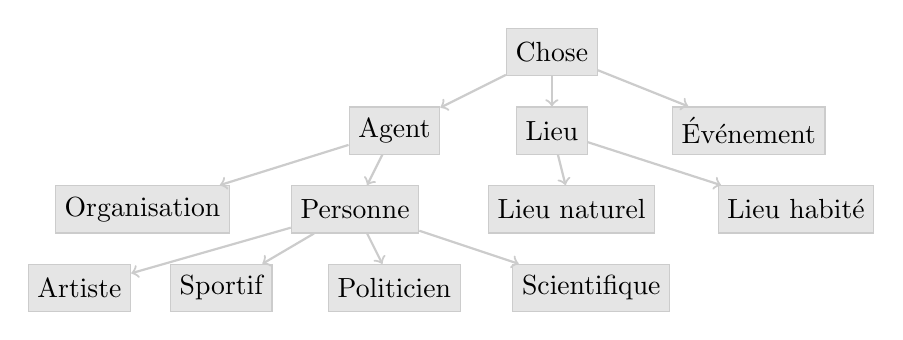
\begin{tikzpicture}[cnode/.style={draw=black,fill=#1,minimum width=3mm,circle},
    rnode/.style={draw=gray!40,fill=gray!20,minimum width=6mm, minimum height=6mm, rectangle}
]
    \node[rnode] (l11) at (0, 0) {Chose};
    \node[rnode] (l21) at (-2, -1) {Agent};
    \node[rnode] (l22) at (0, -1) {Lieu};
    \node[rnode] (l23) at (2.5, -1) {Événement};
    \node[rnode] (l31) at (-5.2, -2) {Organisation};
    \node[rnode] (l32) at (-2.5, -2) {Personne};
    \node[rnode] (l33) at (0.25, -2) {Lieu naturel};
    \node[rnode] (l34) at (3.1, -2) {Lieu habité};
    \node[rnode] (l41) at (-6, -3) {Artiste};
    \node[rnode] (l42) at (-4.2, -3) {Sportif};
    \node[rnode] (l43) at (-2, -3) {Politicien};
    \node[rnode] (l44) at (0.5, -3) {Scientifique};
    \draw[->, gray!40, thick] (l11) -- (l23);
    \draw[->, gray!40, thick] (l11) -- (l21);
    \draw[->, gray!40, thick] (l11) -- (l22);
    \draw[->, gray!40, thick] (l21) -- (l31);
    \draw[->, gray!40, thick] (l21) -- (l32);
    \draw[->, gray!40, thick] (l22) -- (l33);
    \draw[->, gray!40, thick] (l22) -- (l34);
    \draw[->, gray!40, thick] (l32) -- (l41);
    \draw[->, gray!40, thick] (l32) -- (l42);
    \draw[->, gray!40, thick] (l32) -- (l43);
    \draw[->, gray!40, thick] (l32) -- (l44);
\end{tikzpicture}


    \caption{Un exemple de taxonomie généraliste.}
    \label{fig:intro-taxo}
\end{figure}


Pour extraire une taxonomie, on peut s'appuyer sur le contenu d'un graphe de connaissances \cite{cimiano2004conceptual, zhang2019new, volker2011statistical, zhang2019iteratively, ristoski2017large} ou sur un corpus textuel
\cite{wu2008automatically, shwartz-etal-2017-hypernyms, fu2014learning, gupta2016domain, atzori2020fully, pocostales-2016-nuig}. Ce choix d'un graphe ou d'un corpus délimite deux grandes familles d'approches, qui utilisaient à l'origine des méthodes très différentes :
inférence de nouveaux axiomes par des méthodes symboliques ou statistiques dans le premier cas \cite{cimiano2004conceptual, volker2011statistical},  identification de motifs lexico-syntaxiques dans un texte dans le second cas \cite{hearst1992automatic, roller-etal-2018-hearst}. Aujourd'hui, 
on observe une certaine convergence des méthodes grâce à l'utilisation de représentations vectorielles denses des éléments manipulés (qu'il s'agisse d'entités \cite{bordes2013translating}, de mots \cite{mikolov2013distributed} ou de classes \cite{lv2018differentiating}). Ces représentations vectorielles visent à traduire certaines régularités sous forme géométrique, afin que des éléments similaires (par exemple, des mots aux sens apparentés) soient représentés par des vecteurs géométriquement proches. Dans le cas d'un graphe, on parle de \textit{plongements vectoriels de graphe} (ou \textit{knowledge graph embeddings} en anglais); dans le cas du texte, on parle de \textit{plongements lexicaux} (ou \textit{word embeddings} en anglais). Un exemple de tels plongements est représenté à la figure \ref{fig:intro-embeddings}.

%
% illu (PCA of word and graph embeddings FastText/TransE)

\begin{figure}[h]
    \centering
    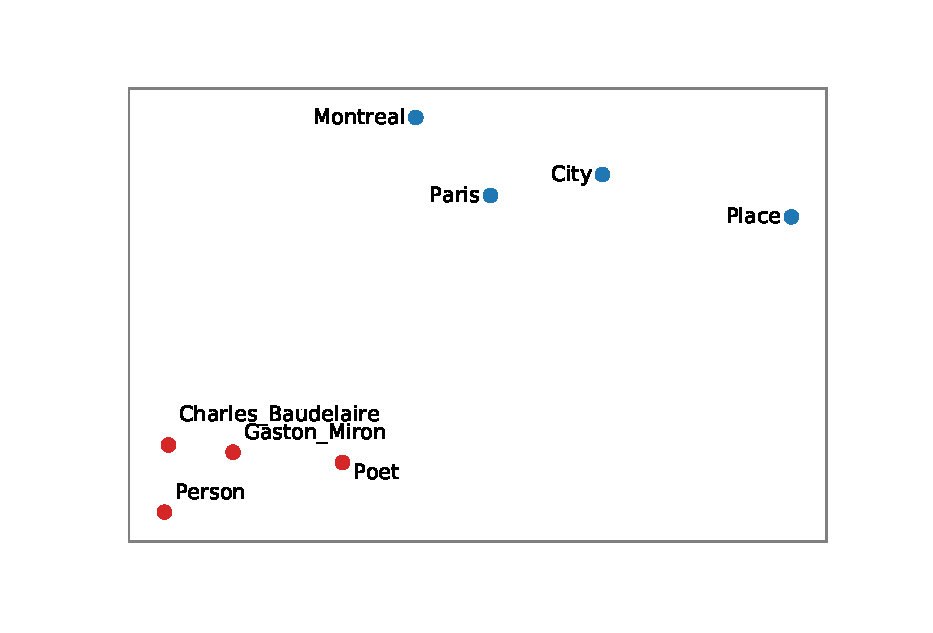
\includegraphics[width=0.7\textwidth]{img/embedding_pca_transe2.eps}
    \caption[Exemple de plongements vectoriels]{
    Un exemple de plongements vectoriels de graphe, représentés en deux dimensions\footnotemark.}
    \label{fig:intro-embeddings}
\end{figure}

\footnotetext{Ces plongements ont été obtenus sur DBpedia \cite{auer2007dbpedia} avec le modèle TransE \cite{bordes2013translating}. Leur dimension est ramenée de $d=50$ à $d=2$ grâce à une PCA.}

Qu'ils soient entraînés sur un graphe ou sur du texte, ces plongements permettent l'application de diverses techniques issues de l'apprentissage automatique au problème de l'extraction de taxonomie, par exemple en entraînant un classificateur capable de détecter la subsomption \cite{fu2014learning}, ou en regroupant les plongements sur la base de leur proximité géométrique \cite{gupta2016domain, zhang2018taxogen}.


Toutefois, la plupart de ces méthodes se contentent d'organiser hiérarchiquement des classes pré-existantes, et ne sont pas capables de caractériser ces classes (que ce soit au moyen d'axiomes logiques, de descriptions textuelles ou même de mots-clés), ni d'identifier de nouvelles classes à partir des données.
%
Dans le présent mémoire, nous proposons au contraire une identification non-supervisée de groupes d'entités cohérents, ce qui permet à la fois de détecter des classes, nouvelles ou pré-existantes, et de les organiser hiérarchiquement au sein d'une taxonomie.

Cette identification se base sur un regroupement hiérarchique ascendant (ou \textit{clustering} hiérarchique) des plongements vectoriels, qui produit un arbre de clustering organisant hiérarchiquement des groupes (ou \textit{clusters}) d'entités en fonction de la distance entre leurs plongements. À partir de cet arbre, on peut produire une taxonomie sur les classes pré-existantes grâce à une méthode d'association entre les classes et les clusters. L'arbre de clustering permet également l'extraction d'une taxonomie \textit{expressive}, c'est-à-dire dont les classes peuvent être soit des classes nommées, soit des classes complexes décrites par des axiomes logiques. Pour ce faire, nous proposons une méthode d'extraction d'axiomes qui cherche spécifiquement à expliquer la partition d'un cluster en deux sous-clusters au sein de l'arbre de clustering. Chacun de ces deux sous-clusters est constitué d'entités géométriquement proches, donc sémantiquement similaires; on exploite donc la géométrie des plongements pour restreindre l'espace de recherche à un sous-ensemble pertinent du graphe. Cette restriction de l'espace de recherche diminue suffisamment la complexité en temps de l'algorithme pour permettre son application à un graphe de grande taille.

%Nous présentons notamment une méthode pour attribuer des axiomes logiques à différents clusters d'un arbre de clustering. Dans un arbre de clustering binaire, chaque cluster (ou groupe d'entité) est divisé en deux sous-clusters

% Couplée à un algorithme d'extraction d'axiome, cette méthode permet 

% Nous montrons d'abord que cette identification non-supervisée est capable de reconstituer une taxonomie sur les classes existantes (c'est le cas non-expressif, décrit au chapitre \ref{chap:te}), puis nous l'utilisons pour extraire de nouvelles classes et les décrire au moyen d'axiomes logiques (c'est le cas expressif, décrit au chapitre \ref{chap:texp}).

% Dans ce travail, nous proposons une identification non-supervisée de groupes d'entités cohérents et pertinents, qui se décline en (a) une variante non-expressive, réclamant peu de données en entrée et (b) une variante expressive, qui utilise tout le graphe de connaissances et permet d'organiser hiérarchiquement les classes entre elles, de décrire les classes existantes au moyen d'axiomes logiques, et d'identifier de nouvelles classes à partir des données.


%%
%% OBJECTIFS DE RECHERCHE / RESEARCH OBJECTIVES
%%
\section{Objectifs de recherche}  % 0.5 page

Dans ce mémoire, nous cherchons à extraire une taxonomie expressive à partir des plongements vectoriels d'un graphe de connaissances.
%
Notre hypothèse est en effet que les plongements vectoriels intègrent dans leur géométrie des notions de proximité entre entités, mais aussi des informations de nature taxonomique, et
%
qu'il doit donc être possible de les utiliser à la fois pour l'identification de groupes d'entités et pour la hiérarchisation de ces groupes. 
%
Notre question de recherche s'énonce donc ainsi :

\begin{quote}
    \emph{Comment les plongements vectoriels de graphe peuvent-ils contribuer à l'extraction de taxonomie ?}
\end{quote}


Pour résoudre ce problème, nous proposons d'utiliser un regroupement hiérachique non-supervisé sur les plongements vectoriels, ce qui permet de créer une structure hiérarchique sur des groupes d'entités. Pour transformer cette structure en une taxonomie expressive ou non-expressive, il est nécessaire de répondre aux sous-questions suivantes :
%
%ce qui suppose de répondre aux sous-questions suivantes :
\begin{quote}
    \emph{\textbf{Q1.} Comment assigner des concepts à des groupes d'entités en tenant compte de la structure d'arbre entre ces groupes ?}
\end{quote}

\begin{quote}
    \emph{\textbf{Q2.} Comment décrire un groupe d'entités à l'aide d'axiomes logiques expressifs ?}
\end{quote}



%%
%% PLAN DU MEMOIRE / THESIS OUTLINE
%%
\section{Plan du mémoire}  % 0.5 page


% On présente d'abord une panorama de la littérature existante. Y sont introduits les concepts fondamentaux du Web sémantique : les graphes de connaissance, qui permettent une représentation structurée de la connaissance, et la logique descriptive, qui permet d'enrichir ces graphes de règles logiques dont la somme constitue une taxonomie ou une ontologie, selon leur complexité. On décrit ensuite les techniques existantes pour extraire automatiquement ces taxonomies, soit à partir d'un graphe, soit à partir de corpus textuels. On propose finalement un survol des méthodes pour inférer de nouveaux axiomes à partir d'un graphe.

On présente d'abord un panorama de la littérature existante au chapitre \ref{chap:revue}. On y introduit les concepts fondamentaux du Web sémantique, et notamment la logique descriptive. On décrit ensuite les techniques existantes pour extraire automatiquement des ontologies ou des taxonomies, que ce soit à partir de textes ou de graphes.

Le chapitre \ref{chap:kge} est consacré aux modèles de plongement, qui permettent une représentation vectorielle des éléments d'un graphe et servent de base à notre travail. On présente plusieurs familles de modèles, et on propose une méthode afin d'identifier le modèle le plus performant pour notre extraction de taxonomie. %pour l'évaluation de ces modèles.


% On présente différents modèles concurrents, en s'efforçant de dégager les intuitions et les hypothèses qui ont dirigé leur conception, et de mettre en évidence leurs limitations théoriques et pratiques. On définit ensuite une nouvelle tâche pour l'évaluation de ces modèles, et on présente les résultats de cette évaluation.


% Dans le chapitre \ref{chap:te}, nous présentons une nouvelle approche pour extraire automatiquement  que 

Les deux chapitres suivants sont consacrés à notre méthodologie d'extraction de taxonomie à partir de graphes. Nous montrons d'abord que le regroupement non-supervisé de plongements vectoriels peut servir à reconstituer une taxonomie sur les classes existantes (chapitre \ref{chap:te}). Pour cela, nous proposons deux méthodes pour assigner un type à des groupes qui émergent d'un processus de regroupement hiérarchique. 
Nous présentons ensuite une méthode pour identifier de nouvelles classes à partir du regroupement non-supervisé, et donc pour produire une taxonomie expressive à partir d'un graphe (chapitre \ref{chap:te}). Cette méthode repose sur un algorithme d'extraction d'axiomes qui exploite le regroupement pour réduire la taille de l'espace de recherche.

%, %
%et qu'il permet de surcroît d'identifier de nouvelles classes, et donc de produire une taxonomie expressive à partir du graphe (chapitre \ref{chap:texp}).

%puis nous l'utilisons pour extraire de nouvelles classes et les décrire au moyen d'axiomes logiques (c'est le cas expressif, décrit au chapitre \ref{chap:texp}).


% on présente une nouvelle approche pour extraire automatiquement une taxonomie à partir des plongements d'un graphe de connaissance. Le chapitre \ref{chap:texp} applique certaines des idées précédentes à l'extraction d'une taxonomie expressive. 
\clearpage       % Introduction au sujet de recherche.
\Chapter{CONTEXTE ET TRAVAUX CONNEXES}\label{chap:revue}

% Text

On présente ici le contexte général de nos travaux, ainsi qu'un aperçu de la littérature existante.
La section \ref{sec:dl} introduit les concepts fondamentaux du Web sémantique : les graphes de connaissances, qui offrent une représentation structurée de la connaissances, et la logique descriptive, qui permet d'enrichir ces graphes de règles logiques dont l'ensemble constitue une taxonomie ou une ontologie, selon les cas.

Nous présentons ensuite les techniques existantes pour extraire automatiquement des taxonomies ou des ontologies. Cette tâche d'extraction automatique a en effet fait l'objet de nombreux travaux : nous résumons ici les principales approches ainsi que les idées notables du domaine, en distinguant notamment les approches basées sur du texte, que l'on présente à la section \ref{subsec:litt-te-text}, et les approches basées sur les graphes, qui sont décrites dans la section \ref{subsec:litt-te-graph}.

Notons enfin que les plongements vectoriels de graphe, qui constituent le socle de notre travail, font l'objet d'un chapitre dédié (chapitre \ref{chap:kge}).


\section{Web sémantique et logique descriptive}
\label{sec:dl}

\subsection{Graphes de connaissances}

% À déplacer vers l'INtroduction ??

%Un graphe de connaissances permet de représenter des données de manière structurée. Il consiste en un ensemble d'objets du monde réel, appellés \textit{entités}, reliés entre eux par des \textit{relations}.

%On se donne $\Ent$ un ensemble d'entités, et $\Rel$ un ensemble de relations. En pratique, chaque entité ou relation est représentée par un identifiant unique, l'IRI (\textit{Universal Resource Identifier}).

%Un graphe de connaissances 

Un graphe de connaissances est une collection structurée de données permettant de représenter des informations, ou des \textit{faits}, sur le monde réel. La définition exacte d'un graphe de connaissances varie d'un auteur à l'autre \cite{ehrlinger2016towards}; parmi les caractéristiques fréquemment retenues, on notera l'interconnexion des données et le caractère multi-relationnel, l'existence d'une sémantique formelle et de mécanismes de raisonnement, et parfois une certaine taille critique. Les paragraphes suivants visent à définir et expliciter ces différentes propriétés.


\paragraph{Concepts de base}

Dans ce travail, on adopte une définition très générale d'un graphe de connaissances vu comme un ensemble d'\textit{entités} liées entre elles par des \textit{relations}. Pour un ensemble d'entités $\Ent$ et un ensemble de relations $\Rel$, un graphe de connaissances est simplement un ensemble de triplets $\KG \subseteq \Ent \times \Rel \times \Ent$. Si $(h, r, t)$ est un triplet du graphe, alors l'entité $h$ est reliée à l'entité $t$ par la relation $r$; dans ce cas, on dit que $h$ est le \textit{sujet} du triplet, et $t$ son objet. Le choix des notations s'explique par l'anglais, $h$ désignant la tête (\textit{head}) et $t$ la queue (\textit{tail}) du triplet. Dans la suite, on désignera par \textit{voisinage} d'une entité l'ensemble des triplets qui impliquent cette entité en tant que sujet ou objet, et on notera $\rel{h}{r}{t}$ pour indiquer que le triplet $(h, r, t)$ est présent dans le graphe.
% Pour un graphe de connaissance, on parle fréquement de données \textit{multi-relationnelles} pour indiquer que les entités

En pratique, lorsqu'on parle de graphe de connaissances, on s'attend à quelques restrictions supplémentaires. D'une part, les données d'un graphe de connaissances doivent être \textit{multi-relationnelles}, c'est-à-dire qu'il doit exister plusieurs relations possibles entre les entités ($| \Rel | > 1$); d'autre part, les entités sont reliées \textit{mutuellement} entre elles. Ainsi, un système reliant des fichiers à des méta-données textuelles ne saurait être qualifié de graphe de connaissances; dans un graphe de connaissances, les objets d'un triplet sont, au moins pour partie, sujets d'autre triplets, et le graphe forme donc un réseau d'entités interconnectées. 


Le format dominant pour représenter un tel graphe est le format RDF, pour \textit{Resource Description Framework} \cite{cyganiak14}. En RDF, les éléments sont de deux types : soit des identifiants, soit des littéraux. Les \textbf{identifants}, ou IRI, pour \textit{International Resource Identifier}, sont simplement des chaînes de caractères qui désignent des ressources du monde réel : lieux, personnes, documents, etc. Les IRI servent également à représenter les relations du graphe.
RDF n'impose pas de mécanisme pour relier les IRI aux entités qu'elles désignent : c'est au créateur du graphe d'établir cette correspondance. Dans le cadre du Web des données, les IRI prennent la forme d'un lien HTTP.
Les \textbf{littéraux} permettent de représenter des valeurs fixes : nombres, textes, booléens, dates, sommes d'argent. Contrairement aux identifiants, l'interprétation des littéraux est définie une fois pour toutes; la manière d'interpréter un littéral est indiquée par son \textit{format} (parfois appelé \textit{datatype} en anglais). Par exemple, le littéral \texttt{1901-01-28\^{}\^{}xsd:date} est constitué de la valeur \texttt{1901-01-28} au format \texttt{xsd:date}, et s'interprète de manière unique comme la date du 28 janvier 1901.

Un \textit{vocabulaire} est un ensemble d'IRI, présentant une certaine cohérence. Les IRI d'un même vocabulaire partagent quasi-systématiquement une racine commune, que l'on peut alors abréger par un \textit{préfixe}. Ainsi, toutes les IRI du vocabulaire standard RDF commencent par \texttt{http://www.w3.org/1999/02/22-rdf-syntax-ns\#}, que l'on abrège en \texttt{rdf:}. Par exemple, les IRI \texttt{http://www.w3.org/1999/02/22-rdf-syntax-ns\#type} et \texttt{http://www.w3.org/199-9/02/22-rdf-syntax-ns\#Property} sont abrégées en \texttt{rdf:type} et \texttt{rdf:Property}, respectivement. 


% De la même manière, les entités de DBpedia sont regroupées dans un vocabulaire commun, dont le préfixe usuel est \texttt{dbr} (abrégé de \texttt{http://dbpedia.org/resource/}) : ainsi, \dbr{Montréal} ou \dbr{Pablo\_Picasso} désignent des entités de DBpedia.

% DBpedia

\paragraph{Un exemple : DBpedia}

Il existe de nombreux graphes de connaissances publics; certains sont restreints à un domaine spécifique, comme UniProt \cite{uniprot2017uniprot} ou DrugBank \cite{wishart2018drugbank}, % WordNet \cite{miller1998wordnet},
d'autres sont généralistes, comme YAGO \cite{suchanek2008yago} ou Wikidata \cite{vrandevcic2014wikidata}. Parmi ces graphes de connaissances généralistes, l'un des plus notables est DBpedia \cite{auer2007dbpedia}, sur lequel on s'appuiera dans toute la suite de ce travail, dans sa version anglaise. Les données de DBpedia sont obtenues de manière automatique en agrégeant différentes sources structurées ou semi-structurées issues de Wikipédia. Le cœur de DBpedia est son système d'extraction, qui convertit Wikipédia en un ensemble de triplets RDF à l'aide de différentes heuristiques; cet extracteur s'appuie essentiellement sur les infoboîtes de Wikipédia, des encarts constituées de paires clé-valeur et dont le format est relativement uniformisé à l'échelle de Wikipédia. Outre les infoboîtes, l'extracteur utilise également les liens de redirection et de désambiguïsation, les catégories des pages, les éventuelles informations de géolocalisation, etc. À cet extracteur s'ajoutent différentes procédures pour nettoyer et uniformiser les résultats, ainsi que pour agréger des données provenant d'autres sources. DBpedia fournit également un point d'entrée pour effectuer des requêtes sur le graphe\footnote{\href{https://dbpedia.org/sparql}{dbpedia.org/sparql}}.

Les entités de DBpedia sont regroupées au sein d'un vocabulaire \texttt{http://dbpedia.org/res-ource/}, généralement abrégé en \dbr{}. Le voisinage d'une entité donnée \dbr{<Nom de l'entité>} %, c'est-à-dire les triplets dont cette entité est le sujet ou l'objet, 
peut être consulté en ligne à l'adresse \href{http://dbpedia.org/page/<Nom de l'entité>}{dbpedia.org/page/<Nom de l'entité>}. Les relations et les classes de DBpedia font elles parties du vocabulaire \texttt{http://dbpedia.org/onto-logy/}, abrégé en \dbo{}. DBpedia fait parfois appel à des relations ou des classes issues d'autres vocabulaires, dont FOAF\footnote{\href{http://xmlns.com/foaf/spec/}{xmlns.com/foaf/spec/}} et Dublin Core\footnote{\href{https://dublincore.org/}{dublincore.org/}}.


Dans la version que nous utilisons, DBpedia contient environ 1 300 relations et 3,4 millions d'entités pour un total de 63,6 millions de triplets. Les entités sont réparties selon 589 types, dont les plus fréquents sont les personnes (\dbo{Person}), les lieux (\dbo{Place}), les espèces (\dbo{Species}), les événements (\dbo{Event}), les œuvres (\dbo{Work}), les organisations (\dbo{Organisation}). Comme les données de DBpedia sont extraites automatiquement de Wikipédia et que Wikipédia est modifié régulièrement, le graphe DBpedia évolue lui aussi régulièrement.


\paragraph{Typologie des relations} 

Il est utile de détailler les propriétés que peuvent avoir les relations dans un graphe de connaissances. Nous citons ici deux propriétés importantes qui serviront dans la suite du mémoire, à savoir la transitivité et la symétrie :
\begin{itemize}
    \item une relation $r$ est \textbf{transitive} si l'existence des liens $\rel{x}{r}{y}$ et $\rel{y}{r}{z}$ implique l'existence de $\rel{x}{r}{z}$ : c'est le cas notamment des relation \dbo{ancestor} et \dbo{isPartOf};
    \item une relation $r$ est \textbf{symétrique} si $\rel{t}{r}{h}$ est vérifiée dès que $\rel{h}{r}{t}$ est vérifiée. Par exemple, la relation \texttt{owl:sameAs}, qui indique que deux IRI correspondent à la même entité, est naturellement symétrique. Plus généralement, toutes les relations qui impliquent une équivalence ou une réciprocité sont symétriques, comme \dbo{spouse} ou \dbo{colleague};
    \item à l'inverse, une relation $r$ est \textbf{antisymétrique} si $\rel{h}{r}{t}$ et $\rel{t}{r}{h}$ ne peuvent jamais être vérifiées simultanément. C'est le cas, en pratique, de la plupart des relations hiérarchiques comme \texttt{rdfs:subClassOf} ou \dbo{parent};
\end{itemize}
Une relation peut très bien n'être ni symétrique, ni antisymétrique. La relation \dbo{influen-cedBy}, qui marque l'influence intellectuelle d'une personne sur un autre, est parfois mutuelle (pensons par exemple à Russell et Wittgenstein, ou Beauvoir et Sartre) et parfois non.


% Une relation est dite \textit{réflexive} si une entité est toujours reliée à elle-même par cette relation, et \textit{irréflexive} si une entité ne peut pas être reliée à elle-même. Par exemple, les relations d'inclusion \texttt{isPartOf} et d'inclusion stricte \texttt{isProperPartOf} entre des ensembles sont respectivement réflexive et irréflexive. Enfin, une relation $r$ est \textit{transitive} si l'existence des liens $\rel{x}{r}{y}$ et $\rel{y}{r}{z}$ implique l'existence de $\rel{x}{r}{z}$ : c'est le cas notamment de la relation \dbo{ancestor}

On peut également classer les relations selon les cardinalités relatives de leurs sujets et de leurs objets :
\begin{itemize}
    \item une relation \textbf{\textit{one-to-many}} (de un à plusieurs, en français) lie chaque sujet à plusieurs objets : par exemple, pour la relation \dbo{product}, 
    une marque est reliée à tous les produits qu'elle commercialise, tandis qu'un produit ne possède qu'une seule marque;
    \item à l'opposé, une relation \textbf{\textit{many-to-one}} (de plusieurs à un) lie plusieurs sujets à un même objet; c'est le cas de la relation \texttt{foaf:gender} qui, dans DBpedia, relie un million et demi de sujets à seulement trois objets (\texttt{"male"}, \texttt{"female"} et \texttt{"non-binary"});
    \item une relation \textbf{\textit{one-to-one}} (un pour un) relie un sujet à un unique objet, et réciproquement. On peut penser à la relation qui unit un pays à sa capitale (\dbo{capital}), ou une entité à son label (\texttt{rdfs:label});
    \item enfin, une relation \textbf{\textit{many-to-many}} (de plusieurs à plusieurs) relie un sujet à plusieurs objets, et un objet à plusieurs sujets. Cette catégorie comprend par exemple la relation \dbo{influencedBy} citée plus haut : en général, un artiste ou un penseur est influencé par plusieurs personnes, et en influence d'autres à son tour;
\end{itemize}

%En parallèle de cette classification stricte des relations, il est parfois intéressant de comparer le
Pour déterminer à quelle catégorie appartient une relation, il suffit de comparer le nombre moyen d'objets par sujet au nombre moyen de sujets par objet \cite{transh}. Pour une relation $r$ donnée, on note $tph_r$ (de l'anglais \textit{tails per head}) le nombre moyen d'objets reliés à une entité par la relation $r$ :
\begin{equation}
    tph_r = \frac{\sum_{h \in \Ent} |\{ t \in \Ent : \rel{h}{r}{t} \}|}{|\{ h \in \Ent : \exists y \in \Ent, \rel{h}{r}{y} \}| }
\end{equation}
Et, réciproquement, on note $hpt_r$ (de l'anglais \textit{heads per tail}) le nombre moyen de sujets qui sont relié à un objet par la relation $r$. 

Dès lors, une relation $r$ est \textit{one-to-many} si $hpt_r = 1$ et $tph_r > 1$, \textit{many-to-one} si $hpt_r > 1$ et $tph_r = 1$, \textit{one-to-one} si $hpt_r = tph_r = 1$, et \textit{many-to-many} si $hpt_r > 1$ et $tph_r > 1$. En pratique, pour les graphes de connaissances extraits automatiquement, cette classification est parfois trop stricte; certains auteurs comme \cite{bordes2013translating, transh} proposent de tenir compte du bruit des données en caractérisant les relations \textit{one-to-many} par $hpt_r \leq 1,5$ et $tph_r > 1,5$, \textit{many-to-one} par $hpt_r > 1,5$ et $tph_r \leq 1,5$, \textit{one-to-one} par $hpt_r \leq 1,5$ et $tph_r \leq  1,5$ et \textit{many-to-many} par $hpt_r > 1,5$ et $tph_r > 1,5$. On désignera cette catégorisation par le qualificatif d'\textit{assouplie}, par opposition à la catégorisation \textit{stricte} présentée plus haut.

La répartition des relations entre les différentes catégories est présentée au tableau \ref{tab:litt-rel-cardinalities}. On peut voir que, au sens strict du terme, les relations \textit{one-to-one}, \textit{one-to-many} et \textit{many-to-one} sont rares; les relations \textit{many-to-many} constituent plus des trois quarts des relations du graphe. En revanche, si l'on assouplit les conditions pour tenir compte du bruit des données, on trouve une majorité de relations \textit{many-to-one} et \textit{one-to-one}. 

%Comparer $hpt_r$ et $tph_r$ permet de

\begin{table}[ht]
    \centering
    \caption{Répartition des différents types de relations dans DBpedia.}
    \begin{tabular}{|l|rr|}
    \hline
& \multicolumn{2}{c|}{Catégorisation} \\
& stricte & assouplie \\ \hline
one-to-one & 7,54\% & 35,39\% \\
one-to-many & 2,54\% & 7,69\% \\
many-to-one & 12,26\% & 46,27\% \\
many-to-many & 77,66\% & 10,66\% \\
\hline
    \end{tabular}
    \label{tab:litt-rel-cardinalities}
\end{table}

Comparer $hpt_r$ et $tph_r$ permet également d'aller au-delà des quatre catégories ci-dessus, et de mieux appréhender la diversité des relations. 
Examinons par exemple les deux relations \textit{many-to-many}  suivantes : \dbo{influencedBy} et \texttt{rdf:type}\footnote{\texttt{rdf:type} est une relation \textit{many-to-many}, car une entité a généralement plusieurs types, et un type a plusieurs instances.}.
Pour la relation \dbo{infl-uencedBy}, on obtient $hpt_r = 2,7$ et $tph_r=2,9$. Autrement dit, une personne est influencée par 2,9 personnes en moyenne, et en influence 2,7\footnote{Plus rigoureusement : une personne qui exerce de l'influence l'exerce en moyenne sur 2,7 personnes; une personne influencée par d'autres est en moyenne influencée par 2,9 personnes.}. On a donc un équilibre entre sujets et objets.
À l'inverse, pour \texttt{rdf:type}, on trouve $tph_r = 3,57$ et $hpt_r = 26 228$ : une entité a en moyenne 3,57 types, et un type a en moyenne 26 228 instances.  
On a donc, dans un cas, un équilibre entre sujets et objets, et de l'autre un net déséquilibre. 
Ces considérations permettent de nuancer les quatres catégories décrites plus haut, et servent notamment au chapitre \ref{chap:kge}, sections \ref{subsec:kge-data-corruption} et \ref{subsec:kge-models-transx}.

%Comme une entité possède en moyenne plusieurs types,  \texttt{rdf:type} est une 

\iffalse {
La caractérisation ci-dessus ne constitue pas une classification formelle des relations, et la frontière entre ces différents types de relation est parfois floue. 

Examinons par exemple la relation \texttt{rdf:type}, fondamentale pour le reste de ce travail, qui associe à chaque entité les types auxquels elle appartient. En général, une entité a plusieurs types : dans DBpedia, \dbr{Gaston\_Miron} possède à la fois les types \dbo{Poet}, \dbo{Person}, \dbo{Agent} et \texttt{owl:Thing}. Réciproquement, de nombreuses entités sont liées à chacun de ces types. On serait donc tenté de catégoriser la relation \texttt{rdf:type} comme une relation \textit{many-to-many}. Pourtant, les effectifs d'un côté et de l'autre sont très déséquilibrés : là où une entité possède au plus sept types distincts, un type peut être relié à des milliers ou des millions d'entités, ce qui apparenterait davantage la relation \texttt{rdf:type} comme une relation \textit{many-to-one}. % Dans le cadre de ce travail, il est plus pertinent de considérer \texttt{rdf:type} comme une relation \textit{many-to-one}.


Examinons par exemple la relation \texttt{rdf:type}, fondamentale pour le reste de ce travail, qui associe à chaque entité les types auxquels elle appartient. En général, une entité a plusieurs types : dans DBpedia, \dbr{Gaston\_Miron} possède à la fois les types \dbo{Poet}, \dbo{Person}, \dbo{Agent} et \texttt{owl:Thing}. Réciproquement, de nombreuses entités sont liées à chacun de ces types. La relation \texttt{rdf:type} est donc une relation \textit{many-to-many}. 
Pourtant, les effectifs d'un côté et de l'autre sont très déséquilibrés : une entité possède en moyenne 3,5 types, alors qu'un type a en moyenne 25 000 instances. Dans certains contextes, il sera plus informatif 
là où une entité possède au plus sept types distincts, un type peut être relié à des milliers ou des millions d'entités, ce qui apparenterait davantage la relation \texttt{rdf:type} comme une relation \textit{many-to-one}.

}
\fi 

\subsection{Ontologies et logique descriptive}

% Présentation

La logique descriptive est un terme général englobant une famille de systèmes logiques, conçus précisément pour décrire des données multi-relationnelles. La logique descriptive cherche à obtenir un compromis entre deux aspects : l'expressivité – la capacité à décrire des situations complexes – et la calculabilité – la possibilité d'effectuer des raisonnements en un temps acceptable. Selon l'équilibre souhaité entre ces deux aspects, on autorise ou non certains types d'axiomes : $\mathcal{SROIQ}$ \cite{horrocks2006sroiq} est le système le plus large et le plus expressif, qui autorise l'ensemble des axiomes de la logique descriptive; $\mathcal{EL}$ et DL-lite sont parmi les plus simples \cite{krotzsch2012owl}; $\mathcal{ALC}$ se situe entre ces deux extrêmes.

%Le choix d'un système logique nécessite un compromis entre deux aspects : l'expressivité et la calculabilité. L'expressivité désigne la capacité à modéliser des situations complexes; la calculabilité concerne 

% On souhaite en effet avoir une expressivité suffisante pour être capable de modéliser logiquement des situations complexes; toutefois, augmenter l'expressivité d'une logique a pour conséquence d'accroître le temps de calcul pour effectuer des raisonnements.


La logique descriptive manipule trois types d'éléments : des entités (ou \textit{individus}), des relations, et des concepts. Les concepts sont des ensembles d'entités, et les relations décrivent des liens entre deux entités. Entités, relations et concepts peuvent être combinés entre eux pour former des \textit{axiomes}; les types de combinaisons possibles varient selon la logique descriptive choisie. Une ontologie (parfois appelée un \textit{schéma}) est alors simplement un ensemble d'axiomes, chacun d'entre eux devant être vrai dans la situation décrite.
Ici, on présente un aperçu des types d'axiomes les plus utilisés; %présentera uniquement les axiomes utilisés dans la suite du mémoire; 
pour une description plus complète, on pourra consulter \cite{krotzsch2013description}. % Il est usuel de distinguer trois grands types d'axiomes : ceux qui expriment 


La forme la plus simple d'un concept est un concept nommé (parfois appelé un \textit{type}), comme par exemple \texttt{Personne}, \texttt{Lieu}, etc. On peut également définir un \textit{concept singleton}, c'est-à-dire un concept contenant une unique instance : $\{ \texttt{alice} \}$ ou $\{ \texttt{bob} \}$ par exemple. Enfin, on dispose de deux concepts spéciaux : le concept universel $\top$, qui contient toutes les entités, et le concept vide $\bot$, qui n'en contient aucune. On peut alors assembler et relier ces différents types de concepts, en utilisant les axiomes qui suivent.

Une première forme d'axiome est la \textbf{subsumption} entre un concept $A$ et un concept $B$, notée $A \sqsubseteq B$, qui indique que les instances de $A$ sont également instances de $B$. Par exemple :
\begin{equation}
    \texttt{Athlète} \sqsubseteq \texttt{Personne}
\end{equation}

On peut aussi indiquer l'\textbf{équivalence} entre deux concepts $A$ et $B$, en écrivant $A \equiv B$. Deux concepts sont équivalents s'ils partagent les mêmes instances, ce qui correspond à une subsumption mutuelle $A \sqsubseteq B$ et $B \sqsubseteq A$. Par exemple :
\begin{equation}
    \texttt{Personne} \equiv \texttt{Humain}
\end{equation}

Pour combiner deux concepts $A$ et $B$, on possède un opérateur de disjonction et un opérateur de conjonction. La \textbf{disjonction} (ou \textit{union)} de $A$ et de $B$, notée $A \sqcup B$, est un nouveau concept qui contient tous les individus qui sont instances de $A$ ou instances de $B$. Cela permet par exemple d'exprimer l'idée qu'un animal est soit un vertébré, soit un invertébré :
\begin{equation}
    \texttt{Animal} \equiv \texttt{Vertébré} \sqcup \texttt{Invertébré}
\end{equation}
La \textbf{conjonction} (ou \textit{intersection}) de $A$ et de $B$, notée $A \sqcap B$, est un concept dont les instances sont tous les individus qui sont à la fois instances de $A$ et instances de $B$. Cela permet d'exprimer des axiomes de la forme :
\begin{equation}
    \texttt{Mère} \equiv \texttt{Parent} \sqcap \texttt{Femme}
\end{equation}

Le \textbf{complémentaire} d'un concept $A$, noté $A^-$, contient l'ensemble des individus qui ne sont pas instances de $A$. On peut ainsi ré-écrire la relation entre vertébrés et invertébrés à l'aide du complémentaire, en disant qu'un invertébré est un animal qui n'est pas vertébré :
\begin{equation}
    \texttt{Invertébré} \equiv \texttt{Animal} \sqcap (\texttt{Vertébré}^-)
\end{equation}

Enfin, on souhaite pouvoir relier les concepts à des relations, et pas seulement les concepts entre eux. Pour cela, on dispose de la \textbf{restriction existentielle} $\exists R.C$, qui représente l'ensemble des individus reliés à une instance de $C$ par la relation $R$. Cela permet par exemple de définir les poètes comme l'ensemble des personnes qui écrivent des poèmes :
\begin{equation}
    \texttt{Poète} \equiv \texttt{Personne} \sqcap \exists \texttt{écrit}.\texttt{Poème}
\end{equation}
L'utilisation d'un concept singleton dans un quantificateur existentiel, qui donne un axiome de la forme $\exists R.\{ e \}$, permet de représenter tous les individus reliés à l'individu $e$ par la relation $R$, par exemple :
\begin{equation}
    \texttt{PoèteCanadien} \equiv \texttt{Poète} \sqcap \exists  \texttt{nationalité}. \{\texttt{Canada} \}
\end{equation}

Enfin, si l'on souhaite seulement représenter les individus qui sont sujets d'une relation, sans restriction sur le type de l'objet associé, on peut utiliser le concept universel :
\begin{equation}
    \texttt{Possédant} \equiv \exists \texttt{possède}.\top
\end{equation}

Il existe également la \textbf{restriction universelle}, notée $\forall R.C$. Un individu $x$ en fait partie à la condition que tous les individus $y$ tels que $\rel{x}{R}{y}$ %auquel il est relié par $R$ 
soient des instances de $C$ (cela inclut donc le cas où $x$ n'est pas sujet de la relation $R$).

Enfin, on peut également obtenir de nouvelles relations à partir de relations existantes. La \textbf{composition de relations}, notée $R_1 \circ R_2$, produit une nouvelle relation qui relie $x$ à $y$ si et seulement si l'on peut trouver $z$ tel que $\rel{x}{R_1}{z}$ et $\rel{z}{R_2}{y}$. L'inverse d'une relation $R$, notée $R^-$ ou parfois $R^{-1}$, est une relation qui relie $x$ à $y$ si et seulement si $y$ est relié à $x$ par $R$.


\paragraph{Sémantique d'une ontologie}

% À partir de maintenant, on désigne par \textit{ontologie} n'importe quel ensemble d'axiomes, et par \textit{taxonomie}, un ensemble d'axiomes de subsumption $A \sqsubset B$. Si on restreint $A$ et $B$ aux seuls concepts nommés, la taxonomie est dite \textit{non-expressive}; sinon, on parlera de taxonomie \textit{expressive}.

On a présenté ici une vision intuitive de la logique descriptive et de ses types d'axiomes. Derrière cette vision intuitive, il existe une sémantique formelle des axiomes logiques et une notion d'interprétation, dont on présente ici les grandes lignes.
Une ontologie correspond à une description partielle du monde; plusieurs états du monde peuvent correspondre à cette description. Une \textit{interprétation} consiste justement à faire correspondre l'ontologie à un état du monde particulier, en reliant chaque entité apparaissant dans l'ontologie à un individu, chaque concept nommé à un ensemble d'individus et chaque relation à un ensemble de paires d'individus. Les axiomes décrits plus haut possèdent tous une \textit{sémantique} formelle, qui est simplement une traduction mathématique ensembliste de la description intuitive qu'on en a fait. Par exemple, la conjonction de concepts $A \sqcap B$ se traduit sémantiquement par l'intersection des ensembles d'individus associés à $A$ et $B$. Cette sémantique permet de vérifier, de façon univoque, si un axiome est vérifié dans l'interprétation choisie. Une interprétation \textit{satisfait} l'ontologie $\mathcal{O}$ si tous les axiomes de $\mathcal{O}$ sont vérifiés; un axiome $\alpha$ est une \textit{conséquence} de cette ontologie s'il est vérifié dans toutes les interprétations qui satisfont $\mathcal{O}$, ce que l'on notera $\mathcal{O} \vdash \alpha$.

On dit qu'une ontologie est \textit{consistante} s'il existe au moins un état du monde (une interprétation) qui satisfait cette ontologie; dans le cas contraire, l'ontologie ne peut jamais être satisfaite, et présente donc peu d'intérêt. Le \textit{raisonnement} logique consiste principalement à vérifier la consistance d'une ontologie d'une part, et d'autre part à déduire de nouveaux axiomes qui sont des conséquences logiques de l'ontologie de départ.


\paragraph{Le formalisme OWL}

Les axiomes de la logique descriptive peuvent être représentés informatiquement dans le langage OWL (\textit{Web Ontology Language}) \cite{Hitzler:12:OWO}, que l'on peut voir comme une extension de RDF pour la représentation d'ontologies. Un axiome de subsumption $A \sqsubset B$ est représenté en OWL par un triplet \texttt{A rdfs:subClassOf B}; l'équivalence $\equiv$, la conjonction $\sqcap$ et la disjonction $\sqcup$ sont représentées respectivement par les relations \texttt{owl:equivalentClass}, \texttt{owl:intersectionOf} et \texttt{owl:unionOf}. %Par rapport à la logique descriptive, OWL ajoute entre autres la gestion des littéraux.

On peut voir un graphe de connaissances comme la combinaison d'un graphe RDF, qui relie les entités entre elles au moyen de relations, et d'une ontologie OWL qui décrit des axiomes reliant les concepts et les relations. Ces deux éléments sont liés entre eux, principalement par la relation \texttt{rdf:type} qui relie les entités (RDF) aux concepts (OWL). La tâche d'extraction d'ontologie, qui fait l'objet de ce mémoire, peut dès lors être vue comme la création ou l'enrichissement de l'ontologie OWL à partir du graphe RDF. Cette division RDF/OWL est parfois simplificatrice, mais elle décrit assez fidèlement le cas de DBpedia et le problème que nous traitons dans ce mémoire.


\section{Extraction automatique d'ontologie et de taxonomie}

% Non ça ça va dans la section 'Problématique' : Constuire une ontologie manuellement est coûteux. Le graphe est dynamique et les données changent bla bla


Le problème d'extraction d'axiomes logiques n'est pas nouveau et prend des formes très variées. Dans le cas général, on cherche soit à construire une ontologie à partir de zéro \cite{lehmann2009dl, joinmerge, petrucci2018expressive, sritha2016survey, volker2011statistical}, soit à étendre une ontologie existante en produisant de nouveaux axiomes \cite{li2019ontology, faralli2017contrastmedium, wu2008automatically}. Un sous-problème fréquent est l'extraction de \textit{taxonomie} \cite{petrucci2018expressive, nickel2018learning, atzori2020fully, ristoski2017large}: il s'agit alors d'extraire uniquement des axiomes de subsumption, c'est-à-dire ayant la forme $A \sqsubseteq B$, afin d'obtenir une hiérarchie sur les concepts. Si on autorise ces concepts à prendre la forme d'axiomes plus complexes, on parlera d'extraction de taxonomie \textit{expressive}. 

On peut distinguer deux grandes familles de méthodes, selon la source des données utilisées : les méthodes basées sur le texte, et les méthodes basées sur un graphe de connaissances. Étant donné la très large disponibilité de corpus textuels étendus (et particulièrement en langue anglaise), les méthodes utilisant le texte sont aujourd'hui les plus fréquentes, et se concentrent particulièrement sur l'extraction de taxonomies. Elles font l'objet de la section \ref{subsec:litt-te-text}. Les méthodes basées sur un graphe ont toutefois leurs avantages : en particulier, elles peuvent fonctionner pour les graphes spécifiques à un domaine et pour lesquels il n'existe pas ou peu de données textuelles. On décrit ces méthodes dans la section \ref{subsec:litt-te-graph}. Notons que l'émergence conjointe des plongements lexicaux (pour le texte) et des plongements vectoriels de graphe permet d'envisager une convergence de ces deux familles de méthodes \cite{nikolaev2020joint}.


\subsection{Extraction d'ontologies à partir de texte}
\label{subsec:litt-te-text}

La recherche de taxonomies ou d'ontologies à partir de textes est explorée depuis longtemps \cite{hearst1992automatic}; aujourd'hui, l'abondance actuelle des ressources textuelles \cite{gigaword2012, smith2013dirt} combinée à l'émergence des plongements lexicaux en ont fait l'approche dominante pour l'extraction de taxonomies : ils nous paraît donc important de la présenter ici.

%De plus, les méthodes basées sur le graphe et basées sur le texte font face à de nombreux problèmes en commun : représentation vectorielle des individus et/ou des concepts, lien entre hiérarchie et géométrie
% Ce problème présente de nombreux points communs avec l'extraction basée sur les graphes; de plus, la combinaison de graphes et de ressources textuelles 
% il nous paraît donc important de présenter ces deux approches.

Dans le contexte textuel, on parle plus volontiers d'\textit{hyperonymie} que de subsumption. Un terme $v$ est un \textit{hyperonyme} d'un terme $u$ s'il est plus général que lui. Dans ce cas, on dit que $u$ est un \textit{hyponyme} de $v$. Par exemple, «animal» est un hyperonyme de «chat», ce qui est analogue à la relation de subsumption $\texttt{Chat} \sqsubseteq \texttt{Animal}$. La principale différence entre l'hyperonymie et la subsumption est que la première concerne indifféremment les entités et les concepts : ainsi, «Garfield» est un hyponyme de «chat», lui-même hyponyme d'«animal». Dans le cas de la subsumption, on distinguerait pourtant ces deux cas, en disant que «Garfield» est une instance de «chat», et «chat» est subsumé par «animal». Cette distinction entre sous-classes et instances est discutée notamment dans \cite{boleda2017instances}.
L'hyperonymie est parfois désignée sous le nom de relation \textit{is-a} («est un», en français) : Garfield \textit{est un} chat, un chat \textit{est un} animal \cite{camacho2018semeval}. 


Les méthodes textuelles pour l'extraction de taxonomie comportent généralement trois étapes : identifier les concepts parmi les mots du vocabulaire, identifier les paires hyponyme-hyperonyme probables, et filtrer ces paires pour obtenir une taxonomie.


\subsubsection{Utilisation de motifs lexico-syntaxiques}

Une première approche consiste à définir des motifs lexico-syntaxiques, appelés motifs de Hearst \cite{hearst1992automatic} (ou \textit{Hearst patterns}, en anglais), pour identifier les relations d'hyperonymie. Par exemple, le motif $NP \texttt{ \{, } NP \texttt{ \}* \{, \} or other } NP$ (où NP indique l'emplacement de noms) trouve une occurrence dans la phrase «\textit{Bruises, wounds, broken bones or other injuries}» et permet de déduire que «\textit{bruise}», \textit{wound}» et «\textit{broken bone}» sont des hyponymes de «\textit{injury}»\footnote{Exemple tiré de \cite{hearst1992automatic}.}.
Ces motifs sont généralement définis à la main, et fixés pendant toute la durée de l'extraction. Toutefois, certaines approches apprennent de nouveaux motifs au cours de l'extraction \cite{snow2005learning, shwartz-etal-2016-improving}. Appliquées à des corpus textuels étendus, les méthodes basées sur des motifs de Hearst ont généralement une bonne précision \cite{roller-etal-2018-hearst}, mais un mauvais rappel \cite{wu2008automatically}, car la langue naturelle présente une grande variabilité et il est difficile de définir des motifs capables de couvrir tous les cas d'hyperonymie.

Les paires hyponyme-hyperonyme extraites sont ensuite filtrées, afin d'éliminer les éventuelles erreurs d'extraction. Dans sa forme la plus simple, le filtrage consiste simplement à compter le nombre d'occurrence de chaque paire, et de définir un seuil minimal. En faisant cela, on pénalise toutefois les mots rares au détriment des mots fréquents : par exemple, il est plus probable d'extraire la paire \textit{(France, pays)} que \textit{(France, république)}, simplement parce que «pays» est un terme plus commun que «république». Pour résoudre ce problème, \cite{turney2001mining} utilise la PPMI (\textit{Positive Pointwise Mutual Information}, ou information mutuelle ponctuelle positive) entre deux termes. Si $w(x, y)$ désigne le nombre d'occurrences d'une paire $(x, y)$ dans les résultats d'extraction, et $W$ le nombre total de paires extraites, on peut définir une fréquence d'extraction $p(x, y) = w(x,y) / W$ pour la paire $(x, y)$; pour le terme $x$, on définit également une fréquence d'apparition en tant qu'hyponyme : $p^-(x) = \sum_y w(x, y) / W$ et en tant qu'hyperonyme : $p^+(x) = \sum_y w(y, x) / W$. La PPMI est alors calculée selon la formule :
\begin{equation}
    PPMI(x, y) = \max \left(0, \log\frac{p(x, y)}{p^-(x)p^+(y)} \right)
\end{equation}

La PPMI permet de résoudre le problème soulevé plus haut : on aura certes toujours $p(\textrm{France}, \allowbreak \textrm{pays}) > p(\textrm{France}, \textrm{république})$, mais également $p^+(\textrm{pays}) > p^+(\textrm{république})$, et donc normalement une PPMI comparable pour les deux paires \textit{(France, pays)} et \textit{(France, république)}.

Enfin, \cite{roller-etal-2018-hearst} propose de lisser les valeurs de PPMI obtenues en réduisant la dimension de la matrice de PPMI avec une SVD tronquée. Cela donne une représentation de rang faible des mots, qui permet alors de décider si deux mots sont hyperonymes l'un de l'autre, même si la paire exacte n'a pas été vue sur le corpus d'entraînement.


Enfin, on peut étendre ces méthodes à l'extraction d'ontologies, et pas simplement de taxonomies. OntoCmaps \cite{zouaq2011towards} effectue pour cela une analyse syntaxique complète des textes traités, et détecte des motifs dans l'arbre syntaxique obtenu. Parmi ces motifs, on trouve les motifs de Hearst décrits plus haut, qui servent à former des liens taxonomiques, mais également des motifs plus complexes, associés à des règles de transformation, qui permettent de transformer des passages textuels en axiomes logiques. 

% Pour améliorer ce rappel, le plus simple est parfois d'améliorer la taille du corpus : (ref) a montré qu'utiliser un ensemble restreint de motifs sur des corpus très étendus permet une bonne extraction. Une autre solution consiste à apprendre de nouveaux motifs au cours de l'extraction \cite{snow2005learning, shwartz-etal-2016-improving}.

\subsubsection{Méthodes distributionnelles, méthodes à plongement}

Les méthodes distributionnelles reposent sur l'«hypothèse d'inclusion distributionnelle» (ou DIH, pour \textit{Distributional Inclusion Hypothesis}) \cite{geffet2005distributional} : si le terme A est un hyperonyme du terme B, alors les contextes dans lesquels B apparaît forment un sous-ensemble des contextes dans lesquels A apparaît. Le contexte d'un mot peut être les $2N$ mots adjacents au sein du corpus ($N$ mots précédents et $N$ mots suivants), ou les éléments voisins (parents ou enfants) au sein d'un arbre de dépendance \cite{shwartz-etal-2017-hypernyms}.
Intuitivement, l'hypothèse DIH signifie que l'on peut remplacer les occurrences de B par A tout en gardant un texte valide.

Pour mettre en pratique cette idée, les méthodes distributionnelles construisent une représentation vectorielles des termes, ou plutôt des contextes des termes; on peut alors évaluer si un terme A est un hyperonyme d'un terme B en utilisant une fonction de classification, qui combine les représentations de A et de B et prédit le résultat. Avant de décrire ces méthodes, il nous faut présenter une étape préalable : l'extraction des concepts.


\paragraph{Extraction des concepts}

L'extraction de taxonomie à partir de texte suppose en effet deux étapes : d'abord, identifier, parmi tous les termes du corpus, ceux qui constituent des concepts; ensuite, identifier les relations d'hyperonymie entre ces concepts. Les méthodes basées sur des motifs de Hearst effectuent simultanément ces deux étapes; ce n'est pas le cas des méthodes distributionnelles, qui supposent une étape préalable d'\textit{extraction des concepts}. Dans certains cas, les concepts sont considérés comme des données d'entrée. %, et l'enjeu est simplement de les ordonner hiérarchiquement. 
Autrement, il est nécessaire de filtrer le corpus, puis d'identifier les concepts : cela consiste généralement à ne garder que les noms, à l'aide d'un étiquettage morpho-syntaxique, puis à les filtrer à l'aide de règles linguistiques ou statistiques \cite{shang2018automated}. % (\hl{ref}).

\paragraph{Approches distributionnelles}

Les approches distributionnelles classiques ne sont pas supervisées \cite{weeds-etal-2004-characterising}, et se fondent sur des représentations creuses des termes. Pour cela, on définit une notion de \textit{co-occurrence}, variable d'un modèle à l'autre : la co-occurrence peut être l'apparition dans une même fenêtre de contexte, ou le fait d'être sujet et objet d'un même verbe dans un arbre de dépendance. Pour un vocabulaire de $N$ termes $\{x_1, \ldots, x_N\}$, on peut alors représenter un terme $t$ par un vecteur $\textbf{t}$ à $N$ dimensions, tel que $\textbf{t}_i$ contient la fréquence de co-occurrence entre $t$ et $x_i$. Pour évaluer si $y$ est un hyperonyme de $x$, on peut alors comparer $\textbf{y}$ et $\textbf{x}$ à l'aide de mesures de similarité usuelles (indice de Jaccard, divergence de Jensen-Shannon ou autre), ou avec des mesures spécifiques à la la recherche de l'hyperonymie, comme la métrique \textit{WeedsPrec} \cite{weeds-etal-2004-characterising} :
\begin{equation}
    WeedsPrec(x, y) = \frac{\displaystyle \sum_{\substack{i=1, \ldots, N \\ \textbf{y}_i > 0}} \textbf{x}_i}{\displaystyle \sum_{i =1, \ldots, N } \textbf{x}_i}
\end{equation}
On retrouve dans cette formule l'hypothèse DIH : si les contextes de $x$ forment un sous-ensemble des contextes de $y$, alors $\textbf{y}_i$ est positif chaque fois que $\textbf{x}_i$ est positif, et on a donc $WeedsPrec(x, y) = 1$. À l'inverse, si les contextes de $x$ et $y$ sont disjoints, on a $WeedsPrec(x, y) = 0$. On peut alors estimer que $y$ est un hyperonyme de $x$ si le score $WeedsPrec(x, y)$ est supérieur à un certain seuil.

\paragraph{Utilisation de plongements lexicaux}
 
Depuis l'introduction de Word2Vec \cite{mikolov2013distributed}, la recherche s'est tournée vers l'exploitation de plongements lexicaux pour représenter vectoriellement les termes. Les plongements lexicaux sont des représentations denses des mots, généralement obtenus à partir de très grands corpus et qui intègrent la sémantique des mots sous forme géométrique.
Deux approches sont possibles : soit utiliser des plongements lexicaux généralistes \cite{fu2014learning, gupta2016domain, atzori2020fully, pocostales-2016-nuig}, soit définir un modèle de plongement lexical spécifique à l'extraction d'hyperonymes \cite{nguyen-etal-2017-hierarchical, nickel2017poincare, nickel2018learning, yu2015learning, luu-etal-2016-learning, vendrov2015order}. 

\textit{Plongements génériques :}
Dans le premier cas, les plongements utilisés sont génériques – typiquement des variantes de Word2Vec. Ils sont donc d'abord conçus pour représenter la \textit{similarité} entre les mots (deux mots apparaissants dans les mêmes contextes auront des plongements géométriquement proches), sans notion de hiérarchie ou d'hyperonymie. Pour identifier l'hyperonymie, \cite{fu2014learning} utilise une méthode supervisée : l'idée est d'apprendre une relation linéaire entre les plongements des hyponymes et ceux des hyperonymes. On dispose de paires d'hyponymes-hypernymes $\{(x_k, y_k )\}$, d'un plongement lexical $\textbf{w}$ pour chaque mot $w$ du vocabulaire, et on souhaite trouver une matrice $\textbf{M}$ telle que $\textbf{M} \textbf{x}_k \approx \textbf{y}_k$, ce qui correspond à un problème classique de régression linéaire. En pratique, une unique relation linéaire est insuffisante pour couvrir la variété des paires d'hyperonymes, et on utilise donc une relation linéaire par morceaux : chaque paire $(x_k, y_k)$ est représentée par le vecteur $\textbf{u}_k = \textbf{x}_k - \textbf{y}_k$, les vecteurs $\textbf{u}_k$ sont alors regroupés en $m$ groupes $C_1, \ldots, C_m$ avec l'algorithme des $k$-moyennes, et une régression linéaire $\textbf{M}_i$ est apprise sur chaque groupe $C_i$. Les $k$-moyennes produisent un partitionnement de l'espace : pour classifier une paire inconnue $(x, y)$, il suffit donc de trouver le groupe $C_i$ auquel la paire appartient, puis de mesurer la distance entre $\textbf{M}_i \textbf{x}$ et $\textbf{y}$ : si elle est inférieure à un certain seuil, alors $y$ est un hyperonyme de $x$.

% Présenter Gupta et Atzori

\textit{Plongements spécifiques :}
Lorsqu'on choisit, au contraire, de définir un modèle de plongement lexical spécifique à la recherche d'hyperonymes, l'enjeu est de trouver une géométrie capable de représenter la notion de hiérarchie. La méthode du \textit{Dynamic-weighting Neural Network} \cite{luu-etal-2016-learning} utilise en entrée une liste de paires hyponymes-hypernymes et un corpus textuel étendu : chaque fois qu'un hyponyme et un hypernyme sont trouvés dans la même phrase du corpus, on extrait un triplet d'entraînement comportant lesdits hyponyme et hypernyme, ainsi que les mots contextuels, c'est-à-dire tous les mots situés entre l'hyponyme et l'hypernyme. On fournit alors ces mots contextuels et l'hyponyme à un réseau de neurone, dont l'objectif est de prédire l'hypernyme. Comme dans Word2Vec, les poids de ce réseau servent alors de plongements lexicaux. HyperVec \cite{nguyen-etal-2017-hierarchical} utilise également une liste de paires hyponymes-hyperonymes et un corpus textuel pour apprendre des plongements lexicaux présentant les caractéristiques suivantes : (a) un hyponyme et un hyperonyme ont des plongements proches au sens de la similarité cosinus, et (b) le plongement d'un hyponyme a une norme euclidienne inférieure à ses hyperonymes.

Une approche classique consiste à choisir un espace $D$ pour les plongements (typiquement l'espace euclidien à $d$ dimensions) et un ordre partiel $\preceq$ sur cet espace, puis à entraîner les plongements lexicaux tels que $\textbf{x} \preceq \textbf{y}$ si $y$ est un hyperonyme de $x$.
Si l'on adopte ce paradigme, il devient intéressant de raisonner avec des \textit{zones d'hyponymie} : la zone d'hyponymie $Z(\textbf{y})$ associée à un plongement $\textbf{y}$ est l'ensemble des points $\textbf{x}$ de $D$ tels que $\textbf{x} \preceq \textbf{y}$. Dès lors, un terme $x$ est un hyponyme de $y$ si son plongement est contenu dans la zone d'hyponymie de $y$. De plus, par transitivité de $\preceq$, on a une équivalence entre $\textbf{x} \preceq \textbf{y}$ et $Z(\textbf{x}) \subseteq Z(\textbf{y})$. Ce cadre permet de visualiser et de comparer plusieurs géométries de plongement : on donne trois exemples de géométries, et on illustre les zones d'hyponymies associées à ces trois choix à la figure \ref{fig:litt-emb-models}.

Le modèle des \textit{Order Embeddings}\cite{vendrov2015order} utilise comme ordre partiel sur $\R^d_+$ la relation :
\begin{equation}
    \textbf{x} \preceq \textbf{y} \iff \forall i = 1, \ldots, d, {} x_i \geq y_i
\end{equation}
En particulier, l'élément racine de la taxonomie aura un plongement nul. %, et chaque plongement définit une \textit{zone d'hyponymie}, c'est-à-dire une zone de l'espace qui contient tous les éléments qui lui sont inférieurs, et donc l'ensemble de ses hyponymes. 
En dimension 2, la zone d'hyponymie d'un point $A$ est le quart de plan supérieur droit de $A$, c'est-à-dire l'ensemble des points situés en haut à droite de $A$ (figure \ref{subfig:orderemb}). Ce choix de $\preceq$ a un inconvénient : il interdit d'avoir des classes disjointes. En effet, quels que soient les plongements $\textbf{x}$ et $\textbf{y}$ considérés, leurs zones d'hyponymies auront une intersection non-vide.

Pour dépasser ce problème, le modèle des \textit{Box-Lattice Embeddings} \cite{vilnis2018probabilistic} se place dans l'hypercube $[0, 1]^d$, c'est-à-dire l'ensemble des vecteurs de $\R^d$ dont toutes les coordonnées sont comprises entre $0$ et $1$, et représente chaque terme $x$ par deux plongements $\textbf{x}^m$ et $\textbf{x}^M$, qui vérifient $x_i^m < x_i^M$ pour tous $i = 1, \ldots, d$. La relation d'ordre entre deux paires de plongement s'écrit :
\begin{equation}
    (\textbf{x}^m, \textbf{x}^M) \preceq (\textbf{y}^m, \textbf{y}^M) \iff \forall i = 1, \ldots, d, {} y_i^m \leq x_i^m < x_i^M \leq x_i^M
\end{equation}
Ce choix de relation d'ordre consiste en fait à choisir comme zones d'hyponymie des pavés de $\R^d$ :
\begin{equation}
    Z(\textbf{x}) = \{ \textbf{u} \in [0, 1]^d : \forall i=1, \ldots, d, {} x_i^m \leq u_i \leq x_i^M \}
\end{equation}
À nouveau, la relation d'hyperonymie entre deux termes se traduit par une relation d'inclusion entre leurs pavés : $y$ est un hyperonyme de $x$ si et seulement si $Z(\textbf{x}) \subseteq Z(\textbf{y})$. La figure \ref{subfig:boxlatticeemb} en donne une illustration.

Enfin, plusieurs travaux ont suggéré de quitter l'espace euclidien et de privilégier un espace hyperbolique \cite{nickel2017poincare, nickel2018learning, Aly_2019, dhingra2018embedding, ganea2018hyperbolic}, qui offre une représentation naturelle des relations hiérarchiques. Comme montré par \cite{ganea2018hyperbolic}, un plongement $\textbf{u}$ dans une boule de Poincaré induit naturellement une zone d'hyponymie conique, dont la largeur dépend de la norme de $\textbf{u}$. Des exemples de ces «cônes d'hyponymie» sont donnés à la figure \ref{subfig:poincone}.


\begin{figure}[h]
    \begin{subfigure}{.32\textwidth}
          \centering
          % include first image
          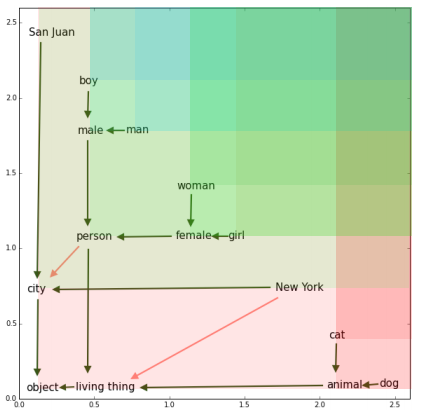
\includegraphics[width=.8\linewidth]{img/orderembboxed.png}  
          \caption{\textit{Order Embeddings}}
          \label{subfig:orderemb}
    \end{subfigure}
    \begin{subfigure}{.33\textwidth}
          \centering
          % include first image
          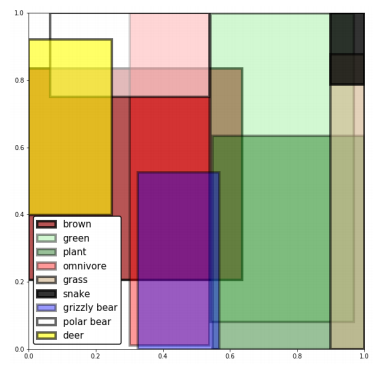
\includegraphics[width=.8\linewidth]{img/emb-boxlattice.png}  
          \caption{\textit{Box-Lattice Embeddings}}
          \label{subfig:boxlatticeemb}
    \end{subfigure}
    \begin{subfigure}{.33\textwidth}
          \centering
          % include first image
          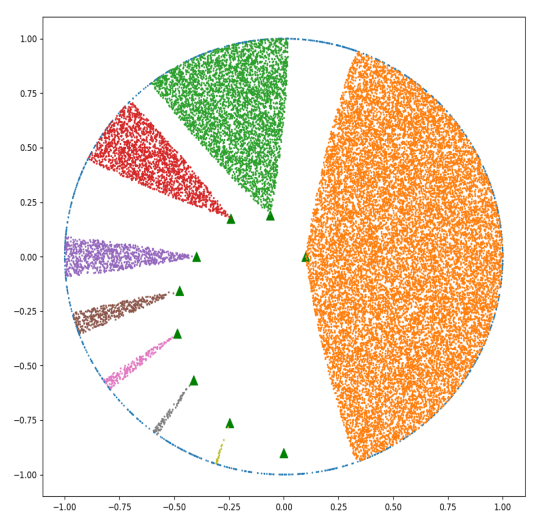
\includegraphics[width=.8\linewidth]{img/emb-poincone.png}  
          \caption{Plongements de Poincaré}
          \label{subfig:poincone}
    \end{subfigure}
    \caption[Plongements lexicaux spécifiques à l'hyperonymie]{Zones d'hyponymies pour  différents modèles de plongement lexical utilisés pour la détection d'hyperonymes. La zone d'hyponymie associée à un concept contient tous les hyponymes de ce concept. Les illustrations proviennent, de gauche à droite, de \cite{vendrov2015order}, \cite{vilnis2018probabilistic} et \cite{ganea2018hyperbolic}.}
    \label{fig:litt-emb-models}
\end{figure}


\subsubsection{Regroupement hiérarchique sur les plongements lexicaux}

Parmi les méthodes qui reposent sur des plongements lexicaux, on s'intéresse ici à celles qui réalisent un regroupement ou partitionnement des données (en anglais : \textit{clustering}).

Un algorithme de regroupement hiérarchique aboutit à la même structure d'arbre qu'une taxonomie : une fois que l'on dispose de représentations vectorielles pour les concepts à hiérarchiser, il est donc naturel d'appliquer un tel algorithme pour obtenir une taxonomie. Plusieurs méthodes ont été proposées dans ce sens. \cite{gupta2016domain} propose un partitionnement divisif de plongements lexicaux : on part de l'ensemble de tous les concepts, représentés par des plongements lexicaux génériques, et on y applique la méthode des $k$-moyennes. Le nombre de clusters $k$ est obtenu de manière non-supervisée, en combinant plusieurs métriques classiques telles que le
critère du coude (en anglais : \textit{elbow method}), la statistique du \textit{gap} et l'examen de la \textit{silhouette} (voir \cite[p.~126--130]{everitt2011cluster} pour une discussion sur ces métriques). Chaque cluster est alors étiquetté à l'aide d'une combinaison de motifs de Hearst, d'analyse statistique et de supervision humaine. Cette nouvelle étiquette est soit l'un des concepts contenus dans le cluster, soit un nouveau nom fourni par un annotateur humain. Puisque la méthode demande une supervision humaine, elle ne résout pas la question cruciale de l'étiquettage automatique des clusters, que nous examinons dans ce mémoire, dans les sections \ref{subsec:te-mapping} (cas non-expressif) et \ref{subsec:texp-exaxiom} (cas expressif). TaxoGen \cite{zhang2018taxogen} propose une méthode pour extraire une taxonomie à partir d'un regroupement hiérarchique de plongements vectoriels. TaxoGen repose sur un partitionnement adaptatif des données, capable de décider, pour chaque cluster, si une instance doit être propagée vers les sous-clusters (c'est-à-dire qu'elle peut être rattachée à un concept plus spécifique que le concept associé au cluster courant), ou si elle doit rester dans le cluster courant (ce qui signifie qu'elle n'est instance d'aucun concept plus spécifique). En revanche, TaxoGen ne propose pas de mécanisme pour associer un nom à chaque cluster : le résultat est donc une hiérarchie de groupes d'instances, et pas un ensemble d'axiomes de subsumption. À nouveau, la question de l'étiquettage automatique des clusters n'est pas résolue.
VDGEC \cite{zhang2018variational2} extrait de corpus textuels un graphe de co-occurrence de concepts, qui relie entre eux les concepts apparaissants fréquemment ensembles. Ce graphe est alors utilisé pour calculer des représentations vectorielles des concepts; ces vecteurs sont ensuite regroupés hiérarchiquement pour donner une taxonomie. La différence essentielle entre la méthode VDGEC et la nôtre est la nature des plongements vectoriels manipulés : dans VDGEC, on utilise directement les \textit{concepts}, alors que nous utilisons les \textit{instances}. Manipuler les instances ajoute une complexité supplémentaire, puisque les données à manipuler sont plus nombreuses, et qu'il est nécessaire de concevoir un mécanisme pour relier chaque concept à un groupe d'instances; en contrepartie, cela autorise une plus grande souplesse, particulièrement en permettant d'identifier de nouveaux groupes d'instances pertinents, et donc de nouveaux concepts. Nous démontrons cette possibilité dans le chapitre \ref{chap:texp}.

%\subsubsection{Extraction d'ontologies à partir de texte}
%Text2Onto, OntoCmaps, OntoGen
%Au-delà de l'extraction de taxonomies, plusieurs méthodes ont été proposées pour extraire directement des ontologies à partir de textes \cite{cimiano2005text2onto, zouaq2011towards, fortuna2007ontogen, haidar2016automatic}. Une approche fructueuse consiste à effectuer une analyse syntaxique des textes traités et à identifier des motifs à partir de l'arbre syntaxique obtenu. Ces motifs incluent les motifs de Hearst cités plus haut, qui servent à former des liens taxonomiques, mais ils sont étendus à d'autres types de relation. 
%La plupart de ces méthodes sont semi-automatiques \cite{cimiano2005text2onto, zouaq2011towards, fortuna2007ontogen}, c'est-à-dire qu'elles 


% \cite{petrucci2018expressive} propose d'appliquer les techniques développées pour la traduction automatique du langage naturel au problème de l'extraction d'axiomes : le but est de traduire une phrase en langage naturel vers la logique descriptive à l'aide d'un réseau de neurone récurrent. Par exemple, la phrase «une abeille est un insecte qui produit du miel» devrait être traduite en $\texttt{Abeille} \sqsubset \texttt{Insecte} \sqcap \exists \texttt{produit} . \texttt{Miel}$. Cette approche est toutefois limité par la rareté des données : il n'existe pas de corpus étendu établissant une correspondance entre langue naturelle et logique, ce qui conduit à des performances assez faibles.



\subsection{Extraction d'ontologies à partir d'un graphe}
\label{subsec:litt-te-graph}


% \hl{Bla bla extraction à partir de graphe}
% On présente d'abord les méthodes symboliques, qui utilisent les règles et le formalisme de la logique. Ces méthodes sont pour la plupart mal adaptées aux graphes de connaissances créés automatiquement ou semi-automatiquement, et ce pour deux raisons essentielles : d'une part, ces méthodes demandent beaucoup de ressources, et ne fonctionnent que sur des ontologies réduites; d'autre part, elles sont incapables de gérer correctement l'incertitude et le bruit qui caractérise ces graphes. 

Ici, on décrit les approches existantes pour extraire ou étendre une ontologie à partir d'un graphe de connaissances. % Là où les approches textuelles sont limitées à l'apprentissage de taxonomie, les méthodes basées sur les graphes permettent plus facilement d'extraire des axiomes expressifs. 
Par rapport à l'utilisation de corpus textuels, l'utilisation d'un graphe permet d'éviter les ambiguïtés syntaxiques ou lexicales, puisque l'on travaille directement à partir de données structurées.
On cherche généralement à exprimer les axiomes extraits dans le formalisme de la logique descriptive; certaines des méthodes présentées ici utilisent d'autres systèmes logiques (règles d'association, programme logique); sous réserve que ces systèmes sont moins expressifs que la logique descriptive $\mathcal{SROIQ}$, le passage de l'un à l'autre ne pose pas de problème.

Une première approche consiste à utiliser des techniques issues de l'intelligence artificielle symbolique pour effectuer des raisonnements à partir de règles existantes et déduire de nouveaux axiomes. D'autres méthodes identifient au contraire des régularités dans le graphe, soit par un examen statistique (fréquences relatives des relations et des concepts, calculs de co-occurrences), soit en plongeant les éléments du graphe dans une espace vectoriel qui reflète la structure du graphe. Ces différentes méthodes sont décrites dans les sections suivantes.


\subsubsection{Méthodes symboliques}

Les méthodes symboliques constituent une première famille d'approches capables de construire de nouveaux axiomes à partir d'axiomes existants. On désigne sous ce nom toutes les méthodes qui manipulent directement des règles logiques.
Ces méthodes sont pour la plupart mal adaptées aux graphes de connaissances créés automatiquement ou semi-automatiquement, et ce pour deux raisons essentielles : d'une part, ces méthodes demandent beaucoup de ressources, et ne fonctionnent que sur des ontologies réduites; d'autre part, elles sont incapables de gérer correctement l'incomplétude et le bruit qui caractérise ces graphes.  On en présente succintement trois grandes familles dans les paragraphes qui suivent.

Les \textbf{raisonneurs}, comme Fact++ \cite{tsarkov2006fact++} ou Hermit \cite{glimm2014hermit}, appliquent des règles de démonstration pour déduire des axiomes nouveaux. Un exemple de ces règles de démonstration est le \textit{modus ponens}, qui consiste simplement en $P \land (P \implies Q) \vdash Q$ : si $P$ est vraie et $P$ implique $Q$, alors $Q$ est vraie. Ces raisonneurs peuvent être utiles pour vérifier si une ontologie donnée est consistante, mais ils ne peuvent pas réellement être utilisés pour l'extraction de taxonomie : 
d'une part, ils nécessitent une ontologie de départ; d'autre part, ce sont des méthodes \textit{déductives} et donc incapables d'inférer de nouvelles règles à partir des données. %; enfin, la complexité de calcul augmente rapidement, ce qui les rend inadaptés pour des ontologies de grande taille.

Une autre approche symbolique \cite{cropper2020turning} est la \textbf{programmation logique inductive} (ou ILP, pour \textit{Inductive Logic Programming}) \cite{nienhuys1997foundations, de2008probabilistic}: il s'agit cette fois d'une méthode \textit{inductive}, c'est-à-dire qui produit de nouveaux axiomes à partir d'exemples. La programmation logique inductive part d'une série d'axiomes (la \textit{théorie préalable}, éventuellement vide) et d'exemples positifs et négatifs; elle cherche à produire de nouveaux axiomes qui sont vérifiés par les exemples positifs  mais pas par les exemples négatifs. De manière informelle et à titre d'exemple, on se donne une propriété $P$, une théorie préalable vide, un ensemble d'exemples positifs $E^+=\{P(0), P(2), P(4), P(8) \}$ et $E^- = \{ P(1), P(3), P(5) \}$ – autrement dit, $0, 2, 4, 8$ vérifient $P$ et $1, 3, 5$ ne la vérifient pas\footnote{Exemple tiré de \cite{nienhuys1997foundations}.}. Alors, un exemple de théorie induite est donné par :
\begin{align}
    & \textrm{Si } P(x) \textrm{ est vraie, alors } P(x + 2) \textrm{ est vraie.} \\
    & P(0) \textrm{ est vraie.}
\end{align}
Cette théorie ne pourrait être obtenue par un raisonneur, car elle n'est pas une conséquence logique de $E^+$ et de $E^-$ : il s'agit simplement d'une théorie plausible étant donné les faits observés. Pour obtenir des théories induites pertinentes, l'ILP nécessite donc un choix judicieux d'exemples positifs et négatifs.
Pour obtenir une théorie induite, 
on part d'une théorie initiale, possiblement vide, puis on l'améliore itérativement : si elle est trop générale, on la spécialise; si elle est trop spécifique, on la généralise \cite[p. 169]{nienhuys1997foundations}.
%deux approches sont possibles : soit partir d'une théorie très générale et la spécialiser itérativement en ajoutant des axiomes ou en précisant les axiomes existants, soit partir d'une théorie très spécifique et la généraliser itérativement.
En pratique, et comme pour les raisonneurs, les méthodes d'ILP passent difficilement à l'échelle pour les graphes de connaissances de grande taille \cite{srinivasan2012data}, même si des heuristiques moins coûteuses en calcul ont été proposées \cite{zeng2014quickfoil}. De plus, les données d'un graphe réel sont incomplètes et bruitées, une situation pas ou mal gérée par la programmation logique. 

Dans notre mémoire (section \ref{subsec:texp-exaxiom}), nous proposons une méthode d'extraction d'axiomes dont le point de départ est proche de l'ILP : on se donne en effet un ensemble d'exemples positifs et négatifs, et on cherche à trouver des axiomes décrivant l'un et pas l'autre. On résout le problème du passage à l'échelle en restreignant drastiquement l'espace de recherche grâce à l'utilisation de plongements vectoriels et du tirage aléatoire (\textit{sampling}). On reprend l'idée d'une amélioration itérative des axiomes par généralisation/spécialisation, mais on gère le bruit et l'incomplétude des données en utilisant des méthodes statistiques plutôt que symboliques.

Une troisième approche symbolique repose sur l'\textbf{analyse formelle de concept} (AFC, en anglais :  \textit{Formal Concept Analysis}), introduite mathématiquement par \cite{wille1982fca} et appliquée à la construction d'ontologie par \cite{cimiano2004conceptual}. L'AFC considère un ensemble d'entités possédant des attributs, et cherche à produire une hiérarchie de \textit{concepts} : dans ce contexte, un concept est une paire $(A, B)$ où $A$ est un ensemble d'entités et $B$ un ensemble d'attributs tels que $B$ est l'ensemble des attributs vérifiés par tous les éléments de $A$, et inversement $A$ est l'ensemble des entités qui vérifient tous les attributs de $B$. L'ensemble des concepts est muni d'une relation d'ordre $\sqsubseteq$ : on a $(A, B) \sqsubseteq (A', B')$ si $A \subseteq A'$ (ou, de manière équivalente, $B' \subseteq B$), analogue à la subsumption décrite plus haut. Munie de cette relation d'ordre, l'AFC induit naturellement une hiérarchie sur les concepts : l'enjeu est donc de construire une série de concepts pertinents.
Pour obtenir ces concepts, on utilise une règle de dérivation : si $A$ est un ensemble d'entités, on désigne par $A'$ l'ensemble des attributs communs à tous les éléments de $A$; de la même manière, si $B$ est un ensemble d'attributs, on désigne par $B'$ l'ensemble des entités qui possèdent tous les attributs de $B$. En partant d'une entité $x$, on peut ainsi obtenir $\{x\}'$ l'ensemble des attributs de $x$, puis $\{x\}''$ l'ensemble des entités qui ont exactement les mêmes attributs que $x$ : la paire $(\{x\}'', \{x\}' )$ constitue un premier concept. En ajoutant une nouvelle entité $y$ à $\{x\}''$, on obtient un nouvel ensemble d'entités $\{x \}'' \cup \{ y\}$, que l'on peut à nouveau dériver en un ensemble d'attributs  $(\{x \}'' \cup \{ y\})'$, lui-même dérivé pour former un second concept $((\{x \}'' \cup \{ y\})'', (\{x \}'' \cup \{ y\})'\}$; et ainsi de suite. Par ailleurs, un ensemble de concepts $C_1, \ldots, C_N$ possède toujours un \textit{sous-concept commun maximal}, c'est-à-dire le plus grand concept $S$ qui vérifie $\forall i, S \sqsubseteq C_i$. De même, chaque ensemble de concepts possède un \textit{superconcept commun minimal}, c'est-à-dire le plus petit concept $S$ tel que $\forall i, C_i \sqsubseteq S$. De plus, il existe un concept minimal, qui contient tous les attributs (et potentiellement aucune entité), et un concept maximal, qui contient toutes les entités (et potentiellement aucun attribut). 
%Le formalisme de l'AFC possède des soubassements mathématiques bien étudiés, mais la conception d'algorithmes efficaces et appropriés à des graphes de grande taille demeure un problème ouvert
À partir de ces notions, de nombreux algorithmes ont été proposés pour l'identification et la hiérarchisation de concepts \cite{valtchev2001building, nourine1999fast, farach2008linear}; 
toutefois, la conception d'algorithmes efficaces et applicables à grande échelle demeure un problème ouvert %ce problème continue à faire l'objet de recherches actives, notamment pour en réduire la complexité et donc permettre des applications à des jeux de données étendus 
\cite{li2016approximate, zhang2019new}.
L'AFC peut être étendue aux relations binaires, c'est-à-dire à des triplets $(h, r, t)$ où $h, t$ sont des entités reliées par la relation $r$ : on parle alors d'\textbf{analyse relationnelle de concept} (ARC, ou \textit{Relational Concept Analysis} en anglais) \cite{bendaoud2008rcafca}. % Une autre extension de l'AFC consiste à remplacer la logique booléenne usuelle par la logique floue, qui accepte des valeurs de vérité continues entre 0 et 1 et qui permet de mieux modéliser l'incertitude \cite{de2012hierarchical, mao2019construction}.

\subsubsection{Méthodes statistiques}

Les méthodes statistiques visent à extraire des règles logiques en observant des régularités statistiques dans un graphe de connaissances : par exemple, en comptant les co-occurrences de certaines classes ou de certaines relations dans le voisinage d'une entité. 

On présente ici la méthode de \textit{Statistical Schema Induction} (SSI, en français : induction statistique d'ontologie) \cite{volker2011statistical}, qui se rapproche du travail que nous présentons à la section \ref{subsec:texp-exaxiom}. Cette approche repose sur l'apprentissage de \textit{règles d'association} \cite{zhang2003association}, qui sont essentiellement des implications logiques inférées d'après des co-occurrences observées dans les données. 
Une règle d'association s'écrit sous la forme $X \rightarrow Y$. On peut par exemple imaginer une règle $\{\texttt{Personne}, \exists \texttt{écrit}.\texttt{Poème} \} \rightarrow \texttt{Poet}$ : si une même entité est de type \texttt{Personne} et vérifie l'axiome $\exists \texttt{écrit}.\texttt{Poème}$, alors cette entité est probablement de type \texttt{Poète}.

Pour extraire ces règles, on se donne un \textit{tableau de transactions} $\textbf{T}$, c'est-à-dire une matrice dont les lignes représentent les entités $e_1, \ldots, e_n$ du graphe, et les colonnes des prédicats logiques $P_1, \ldots, P_m$. Ces prédicats incluent les concepts nommés $C$ (comme \texttt{Artist}, \texttt{Person}, etc.) et différentes formes de restrictions existentielles comme $\exists r.C$ ou  $\exists r.\top$. On note $\Ent$ l'ensemble des entités, et $\mathcal{P}$ l'ensemble des prédicats. 
La coordonnée $(i, j)$ de $\textbf{T}$ contient $1$ si $e_i$ vérifie le prédicat $P_j$, et $0$ sinon. Soit $X \subseteq \mathcal{P}$ un ensemble de prédicats, alors le \textit{support} de X est l'ensemble des entités qui vérifient tous ces prédicats simultanément :
\begin{equation}
    \textrm{Supp}(X) = \frac{|\{ e \in \Ent : \forall P \in X, P(e) \}|}{|\Ent |}
\end{equation}
L'indice de confiance associée à une règle $X \rightarrow Y$ se calcule alors par :
\begin{equation}
    \textrm{Conf}(X \rightarrow Y) = \frac{\textrm{Supp}(X \cup Y)}{\textrm{Supp}(X)}
\end{equation}
Au numérateur, on compte le nombre d'entités qui vérifient à la fois les prédicats de $X$ et de $Y$, que l'on rapporte au nombre d'entités qui vérifient les prédicats de $X$ (notons que l'on a nécessairement $\textrm{Supp}(X \cup Y) < \textrm{Supp}(X)$, car une entité qui vérifie à la fois les prédicats de $X$ et de $Y$ vérifie \textit{a fortiori} ceux de $Y$). Un indice égal à $1$ signifie que toutes les entités qui vérifient $X$ vérifient également $Y$, et donc que la règle $X \rightarrow Y$ est parfaitement validée par les données; dans la pratique, on définit plutôt un seuil $\tau$ au-delà duquel la règle d'association est considérée comme valide.

Le nombre de combinaisons de prédicats possibles croît exponentiellement : les énumérer est donc impossible, même pour des jeux de données réduits. Plusieurs heuristiques ont été développées, dont la plus connue est Apriori \cite{srikant1994apriori}, elle-même améliorée à plusieurs reprises, par exemple en minimisant le nombre de lectures du graphe \cite{yuan2017improved} ou en implémentant un mécanisme de parallélisme avec MapReduce \cite{lin2014mapreduce}. % Autres approches : FP-growth, OPUS

Une fois les règles d'association extraites, on peut les filtrer et les convertir en axiomes de subsumption. Cette approche produit des axiomes de subsumption isolés les uns des autres, alors qu'on souhaite généralement obtenir une hiérarchie contenant tous les concepts nommés et, éventuellement, de nouveaux concepts expressifs. Dans notre propre méthode, nous reprenons l'idée d'extraire des axiomes en examinant statistiquement un tableau de co-occurrence entités-axiomes. Notre méthode propose toutefois deux différences essentielles : d'une part, elle s'applique sur un groupe d'entités restreint, qui a été défini de manière non supervisée en se basant sur des plongements vectoriels; d'autre part, l'extraction d'axiomes sert uniquement à \textit{étiquetter} des groupes d'entités, et non pas à obtenir des liens de subsumption. Dans notre cas, les relations de subsumptions sont identifiées par regroupement hiérarchique.



% À partir de textes
% Traduction d'axiomes depuis le langage naturel
\subsubsection{Utilisation de plongements vectoriels de graphe pour l'extraction d'ontologies}

Un modèle de plongement vectoriel de graphe est un modèle capable de construire des représentations vectorielles des entités et des relations d'un graphe de connaissances. Il s'agit d'une approche relativement récente qui présente une analogie forte avec les plongements lexicaux utilisés en traitement de la langue. Les modèles de plongement constituent un aspect important de notre travail, et sont décrits en détail dans le chapitre \ref{chap:kge} – on renvoie donc le lecteur à ce chapitre pour une plus ample présentation. Dans cette section, il suffit de savoir qu'un modèle de plongement associe à chaque entité $e$ du graphe un vecteur $\textbf{e} \in \R^d$ (plus rarement $\mathbb{C}^d$), de telle sorte que deux entités impliquées dans des relations similaires aient des plongements géométriquement proches.

Les plongements vectoriels de graphes de connaissances sont très utilisés pour découvrir des régularités au niveau des instances (ce qui permet notamment d'évaluer la validité d'un triplet inconnu ou de prédire de nouveaux triplets), mais ils ont encore été peu exploités pour la manipulation de concepts ou l'extraction de taxonomie ou d'ontologie. Dans cette optique, \cite{gutierrez2018knowledge} étudie les liens entre les axiomes logiques et la géométrie de différents modèles de plongement, dans le but de pouvoir traduire un axiome sous forme de plongement vectoriel sans perte d'information ou d'expressivité. Une idée qui commence à se développer consiste à utiliser les plongements vectoriels pour évaluer \textit{a priori} la plausibilité d'un axiome logique, ce qui permet de réduire l'espace de recherche. Dans cette lignée, IterE \cite{zhang2019iteratively} apprend conjointement des plongements vectoriels et des règles logiques, les deux se renforçant mutuellement. Des plongements sont initialement appris à partir du graphe de connaissancess; ensuite, une marche aléatoire dans le graphe permet de générer des axiomes potentiels. Ces axiomes se voient alors attribuer un score de vraisemblance, grâce à une table de correspondance entre axiomes logiques et plongements. Par exemple, l'axiome $A \equiv B$ est traduit géométriquement par $\textbf{A} = \textbf{B}$, où $\textbf{A}$ et $\textbf{B}$ sont les plongements vectoriels des concepts $A$ et $B$. Le score de vraisemblance de $A \equiv B$ est alors défini comme la similarité géométrique des plongements de $A$ et de $B$ : dans le cas idéal où $\textbf{A} = \textbf{B}$, la similarité est maximale et l'axiome obtient un score de 1. Plus on s'éloigne de ce cas idéal, plus le score diminue. Cette approche permet une évaluation peu coûteuse des axiomes candidats. Enfin, les axiomes ayant un score de vraisemblance suffisamment haut servent à générer de nouveaux triplets d'entraînement : on peut alors répéter ces trois étapes pour améliorer itérativement les plongements et les axiomes. Cette méthode est uniquement évaluée sur des graphes de petite taille (moins de 50 000 entités); savoir si elle est applicable à plus large échelle reste une question ouverte. RLvLR \cite{omran2018scalable} repose sur un principe similaire. Il cherche à extraire des règles logiques de la forme $x \overset{r_1}{\longrightarrow} z_1 \overset{r_2}{\longrightarrow} z_2  \overset{r_3}{\longrightarrow} \ldots  \overset{r_k}{\longrightarrow} y$ $\implies \rel{x}{r}{y}$. entre les relations. Pour une relation $r$ donnée, on récupère les triplets impliquant $r$, puis on effectue des marches aléatoires autour de ces triplets pour générer des règles candidates. Ces règles sont alors filtrées en exploitant la similarité des plongements des relations impliquées dans chaque règle. Cela permet de restreindre l'espace de recherche et donc d'appliquer la méthode à des graphes de grande taille comme Wikidata ou DBpedia. En contrepartie, l'expressivité des axiomes extraits est limitée; de plus, les axiomes extraits ne sont pas organisés entre eux sous forme de taxonomie.


\phantomsection
\label{subsec:litt-tiemb}


Plus proche de notre propre méthode, \textbf{TIEmb} \cite{ristoski2017large} extrait une taxonomie (non-expressive) à partir de plongements vectoriels d'entités. Comme notre méthode, TIEmb considère comme données d'entrée un ensemble de paires $\{(\textbf{e}_i, t_i) \}_{i=1, \ldots, n}$, où $\textbf{e}_i \in \R^d$ est le plongement vectoriel de l'entité $e_i$, et $t_i$ est son type, et produit en sortie une taxonomie, c'est-à-dire un ensemble d'axiomes de subsumption de la forme $t_i \sqsubset t_j$. Pour cela, chaque type $t$ est représenté par un sphère $S_t$ à $d$ dimensions, dont le centre est un vecteur $\textbf{c}_t$ défini par :
\begin{equation}
 \textbf{c}_t = \frac{1}{n_t} \sum_{\substack{i \in [1, n] \\ t_i = t}} \textbf{e}_i
\end{equation}
Avec $n_t = |\{ i \in [1, n] : t_i = t \}|$ le nombre d'entités de type $t$ dans les données. $\textbf{c}_t$ représente le centroïde des instances de $t$.

Le rayon $r_t$ de $S_t$ est lui défini comme la distance moyenne entre les instances de $t$ et le centroïde $\textbf{c}_t$ :
\begin{equation}
    r_t = \frac{1}{n_t}  \sum_{\substack{i \in [1, n] \\ t_i = t}} \| \textbf{e}_i - \textbf{c}_t \|_2
\end{equation}


\begin{figure}[h]
    \centering
    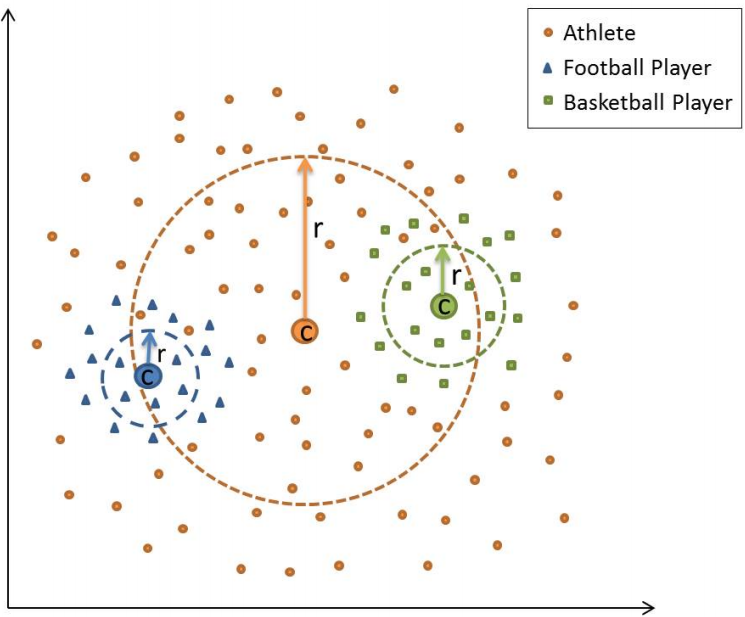
\includegraphics[width=0.5\textwidth]{img/tiemb.png}
    \caption[Principe général de TIEmb]{Plongements et sphères associées à trois classes dans le cadre de la méthode TIEmb, dans le cas bidimensionnel. Illustration tirée de \cite{ristoski2017large}.}
    \label{fig:litt-tiemb}
\end{figure}


Dès lors, l'axiome $t \sqsubset t'$ est prédit si et seulement si $S_t \subset S_{t'}$ : la sphère d'un supertype englobe les sphères de ses sous-types, comme illustré à la figure \ref{fig:litt-tiemb}. Enfin, une étape finale de filtrage est appliquée pour enlever les cycles et obtenir une taxonomie valide. 

TIEmb présente l'avantage d'être conceptuellement simple, et peu coûteux en calcul, ce qui permet de l'appliquer à très grande échelle. Une différence cruciale avec notre approche est que le regroupement des entités au sein des sphères est entièrement supervisé, puisqu'il repose sur les types $t_i$ contenus dans les données, et pas sur la géométrie des plongements : TIEmb ne permet donc pas d'identifier de nouveaux groupes cohérents d'entités et donc de détecter de nouvelles classes. Dans le chapitre \ref{chap:te}, on compare notre méthode d'extraction de taxonomie non-expressive à TIEmb; dans le chapitre \ref{chap:texp}, on illustre les possibilités offertes par le regroupement non-supervisé en extrayant une taxonomie expressive de DBpedia.

\paragraph{Résumé}

On a présenté un aperçu de différentes approches pour extraire automatiquement des taxonomies ou des ontologies. Parmi ces méthodes, celles qui manipulent directement un graphe ou des textes se heurtent à deux difficultés : d'une part, les données sont \textit{sparse} (parfoit traduit par «disséminées» ou «creuses» en français), c'est-à-dire que de nombreux éléments (mots ou entités) sont rarement observés; d'autre part, les données sont \textit{discrètes}, et généraliser les observations faites sur un élément à d'autres éléments est compliqué.

Les plongements vectoriels permettent de surmonter ces deux difficultés, et ont été appliqués à l'extraction d'ontologies avec une grande variété de méthodes et d'objectifs.
Toutefois, aucune des méthodes présentées ne permet d'extraire une ontologie complète et de haute qualité sans supervision humaine. %Le problème demeure donc ouvert. 
Les modèles capables d'induction complexe ne sont généralement pas applicables sur des graphes de grande taille comme DBpedia. À l'inverse, les modèles capables de passer à l'échelle se contentent de hiérarchiser des classes existantes, et sont incapables d'identifier de nouvelles classes à partir des données. 
Dans la suite, nous proposons une méthode capable d'extraire une taxonomie expressive à grande échelle, en combinant plongements vectoriels de graphe, regroupement hiérarchique non-supervisé et extraction d'axiomes à partir de statistiques sur le graphe. Au préalable, nous présentons en détail les modèles de plongement vectoriel dans le chapitre \ref{chap:kge}.  % Revue de littérature.
\Chapter{PLONGEMENTS VECTORIELS DE GRAPHES DE CONNAISSANCES}\label{chap:kge}

\section{Généralités}
\label{sec:kge-general}

\subsection{Introduction, notations et premiers concepts}
\label{subsec:kge-general-intro}

Les graphes de connaissance permettent d'appliquer des algorithmes de raisonnement très puissants. Toutefois, dans les bases de grande taille comme DBpédia ou Wikidata, la complexité en temps de ces algorithmes augmente rapidement, au point de les rendre inutilisables. Hors des algorithmes dédiés, les entités et les relations d'un graphe sont représentés de façon purement symbolique. La nécessité est donc apparue d'obtenir une représentation plus expressive des entités et relations d'un graphe. Pour ce faire, et suivant la dynamique du traitement automatique des langues, on a recours à des modèles de plongement. 

\todo{Reformuler, en partant des différents modes de représentation}

Un modèle de plongement est une méthode pour obtenir des représentations vectorielles denses et sémantiquement cohérentes des entités d'un graphe. Denses, c'est-à-dire de faible dimension, par opposition à une représentation sous forme de matrice d'adjacence $M(h) \in \{0, 1\}^{n_r \times n_e}$ où $M(h)_{i, j} = 1 \iff (h, r_i, e_j) \in \mathcal{KG}$. Sémantiquement cohérentes, car le modèle est construit de façon à envoyer une partie de l'information sémantique contenue dans le graphe vers l'espace vectoriel d'arrivé, afin que des entités sémantiquement proches dans le graphe aient des plongements vectoriels géométriquement proches.

Formellement, un modèle de plongement vectoriel est un modèle qui associe à chaque entité $e \in \mathcal{E}$ un vecteur $\mathbf{e} \in \mathbb{R}^d$, et à chaque relation $r \in \mathcal{R}$ un vecteur $\mathbf{r} \in \mathbb{R}^{d'}$. On note $\mathbf{E} = \{\mathbf{e}\}_{e \in \mathcal{E}} $ l'ensemble des plongements d'entité, $\mathbf{R} = \{\mathbf{r}\}_{r \in \mathcal{R}} $ l'ensemble des plongements de relation et $\Theta = (\mathbf{E}, \mathbf{R})$ l'ensemble des paramètres du modèle. Un modèle de plongement est caractérisé par $\Theta$ ainsi que par une fonction de score $\sigma_{\Theta} : \mathcal{E \times R \times E} \rightarrow [0, 1]$, définie sur l'ensemble des triplets possibles et paramétrée par $\Theta$.  

Pour entraîner un modèle de plongement, on a besoin d'un ensemble de triplets valides $\Delta_+$ (généralement, $\Delta_+ = \mathcal{KG}$), et un ensemble de triplets invalides $\Delta_-$. Comme un graphe ne contient, par construction, aucun triplet invalide, on construit $\Delta_-$ en fabriquant des triplets aléatoirement, et en supposant qu'ils sont invalides – c'est \textit{l'hypothèse du monde localement fermé}, empiriquement vérifiée dans n'importe quel graphe suffisamment grand.
\todo{Ajouter une ref à la section qui le justifie}

Une fois que l'on dispose de $\Delta_+$ et de $\Delta_-$, on peut commencer l'entraînement proprement dit. La procédure varie d'un modèle à l'autre, mais on en présente ici les grandes lignes. Tout d'abord, les paramètres (c'est-à-dire les plongements) sont initialisés aléatoirement. On définit une fonction de perte, typiquement une perte par marge maximale :
$$
J(\Theta) = \sum_{(h_+, r_+, t_+) \in \Delta_+} \sum_{(h_-, r_-, t_-) \in \Delta_-} \lfloor \gamma + \sigma_\Theta(h_+, r_+, t_+) - \sigma_\Theta(h_-, r_-, t_-) \rfloor
$$
On souhaite alors minimiser la perte. Pour cela, on calcule alors $\displaystyle \frac{\partial J}{\partial \Theta}$, et on met à jour $\Theta$ par descente de gradient. Il faut garder à l'esprit que mettre à jour $\Theta$ signifie mettre à jour les plongements vectoriels des entités et des relations du graphe, de façon à avoir un score maximal sur les triplets valides et minimal sur les triplets invalides. La procédure s'arrête une fois un critère de convergence atteint – par exemple, lorsque $J$ ne diminue plus.

Dans la suite de la section, on se propose de détailler plus avant les procédures communes à tous les modèles, et particulièrement la constitution des données d'entraînement, la distinction entre fonction de score et fonction d'énergie, ainsi que les fonctions de pertes communément utilisées. 

\section{Modèles de plongement}
\label{sec:kge-models}

\subsection{Modèles à translation : TransE et ses variantes}
\label{subsec:kge-models-transx}

On présente ici une première famille de modèles, les modèles \textit{à translation}, constituée de TransE et de ses dérivés. L'idée première de ces modèles consiste à représenter une relation entre deux entités comme une translation entre leurs plongements. Une relation $r$ est représentée par une translation $T_r$ de vecteur caractéristique $\mathbf{r}$ :
\begin{equation*}
    T_r : \mathbf{u} \mapsto \mathbf{u + r}
\end{equation*}

Un triplet $(h, r, t)$ est considéré comme valide si le plongement de $t$ est le translaté du plongement de $h$ par la translation $T_r$, c'est-à-dire $T_r(\mathbf{h}) = \mathbf{t}$. La plupart des modèles ajoutent une étape préalable à la translation : le plongement d'une entité $e$ est d'abord envoyé dans un nouvel espace, qui dépend de $r$ et éventuellement de $e$. Ensuite seulement, la translation a lieu dans ce nouvel espace.

Ainsi, on peut définir le cadre générale suivant pour décrire un modèle à translation :
\begin{itemize}
    \item une fonction de transformation $F_{e, r} : \mathbb{R}^d \rightarrow \mathbb{R}^{k}$
    \item une fonction d'énergie $E_\Theta(h, r, t) = \| F_{h, r}(\mathbf{h}) + \mathbf{r} - F_{t, r}(\mathbf{t}) \|_2 $
\end{itemize}

\subsubsection{TransE \cite{bordes2013translating}}
Le premier et le plus simple des modèles à translation, la fonction de transformation est la fonction identité ($\forall e, r, F_{e, r} = I_d$) – autrement dit, les plongements sont translatés directement, sans transformation préalable. En conséquence, les entités et les relations sont plongées dans le même espace $\mathbb{R}^d$, et la fonction d'énergie est donc
\begin{equation}
    E_\Theta(h, r, t) = \| \mathbf{h + r - t} \|_2
    \label{eq:transe-main}
\end{equation}

Le nombre de paramètres est donc $d \times (N + M)$, linéaire en le nombre d'éléments du graphe. 

La force de TransE réside dans sa simplicité théorique et son faible nombre de paramètres. Toutefois, cette simplicité se paye par une faible expressivité, qui limite sa capacité à modéliser des relations autres que \textit{one-to-one} :
\begin{itemize}
    \item relation \textit{many-to-one} : si plusieurs entités $h_1, h_2, \ldots, h_k$ sont reliées à une même entité $t$ par une relation $r$, alors les translatés $\mathbf{h_i + r}$ doivent tous être égaux, donc $\mathbf{h_1  = h_2 = \ldots = h_k}$;
    \item relation \textit{one-to-many} : comme au-dessus, si $h$ est lié par $r$ à plusieurs entités $t_1, \ldots, t_k$, alors nécessairement $\mathbf{t_1 = t_2 = \ldots = t_k}$;
    \item relations symétriques : si $r$ est symétrique, c'est-à-dire $h  \overset{r} \rightarrow t \implies t   \overset{r} \rightarrow h$, alors la translation de la translation par $r$ doit donner l'élément de départ, donc $\mathbf{r} = 0$
\end{itemize}

\subsubsection{TransH \cite{fu2014learning}}

\begin{figure}[hbt]
    \centering
    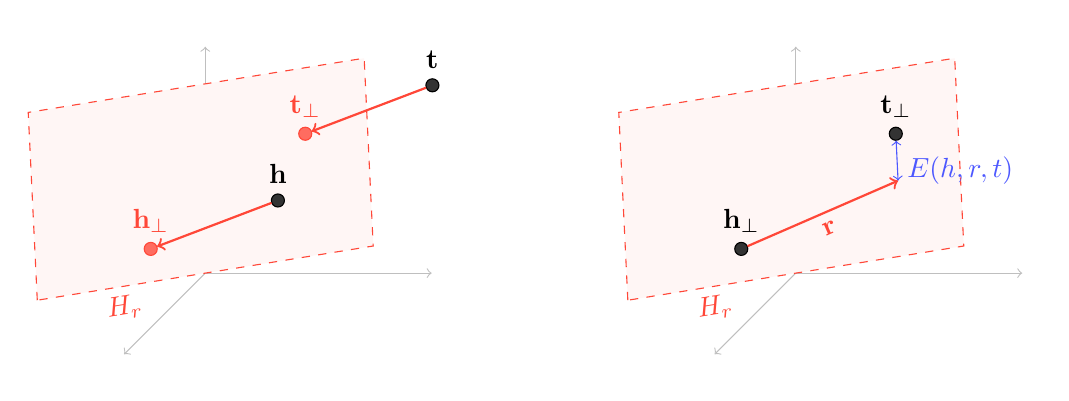
\begin{tikzpicture}
\def\rep{3};
\def\size{1};
\def\px{-0.5*\size};
\def\py{1.5*\size};
\def\pz{-.5*\size};
\def\hplane{(\px, \py, \pz)};

\def\hsize{2};
\def\vsize{2};
\def\offset{0.5};

\tikzmath{
    \base=2;
    \rx=1*\base;
    \ry=0.5*\base;
    \rz=0.5*\base;
    % h_p
    \hp1=-0.5;
    \hp2=0.5;
    \hp3=-(\hp1*\rx+\hp2*\ry)/\rz;
    \h1=\hp1+\rx;
    \h2=\hp2+\ry;
    \h3=\hp3+\rz;
    % t_p
    \tp1=0.5;
    \tp2=1;
    \tp3=-(\tp1*\rx+\tp2*\ry)/\rz;
    \t1=\tp1+\rx;
    \t2=\tp2+\ry;
    \t3=\tp3+\rz;
    % v
    \v1=-sqrt(((\rx)^2) / ((\rx)^2 + (\rz)^2));
    \v2=0;
    \v3=sqrt(((\rz)^2) / ((\rx)^2 + (\rz)^2));
    % u
    \u1=-\ry / (\rx - (\v1 * \rz) / \v3);
    \u2=1;
    \u3=-\u1*\v1/\v3;
}

\newcommand{\makeplane}{
    % Make axis
    \node (o) at (0, 0, 0) {};
    \node (x) at (\rep, 0, 0) {};
    \node (y) at (0, \rep, 0) {};
    \node (z) at (0, 0, \rep) {};
    
    \draw[axis] (o.center) -- (x);
    \draw[axis] (o.center) -- (y);
    \draw[axis] (o.center) -- (z);
    
    % Make plane
    \filldraw[plane] 
    (\hsize*\v1, \hsize*\v2, \hsize*\v3)
    --  ++(\vsize*\u1, \vsize*\u2, \vsize*\u3)
    -- ++(-2*\hsize*\v1, -2*\hsize*\v2, -2*\hsize*\v3)
    -- ++(-\vsize*\u1, -\vsize*\u2, -\vsize*\u3)
    -- node[below, accent1, sloped, near end] {$H_r$} cycle;
}

\begin{scope}
    % Make axis
    \makeplane
    
    \node[node=accent1, label={[accent1]$\bf{h_\bot}$}] (hp) at (\hp1,\hp2,\hp3) {};
    \node[node=black, label={$\bf{h}$}] (h) at (\h1,\h2,\h3) {};
    \draw[accent1, thick, ->] (h) -- (hp);
    
    \node[node=accent1, label={[accent1]$\bf{t_\bot}$}] (tp) at (\tp1,\tp2,\tp3) {};
    \node[node=black, label={$\bf{t}$}] (t) at (\t1,\t2,\t3) {};
    \draw[accent1, thick, ->] (t) -- (tp);
\end{scope}

\begin{scope}[xshift=7.5cm]
    % Make axis
    \makeplane
    
    \node[node=black, label={$\bf{h_\bot}$}] (hp) at (\hp1,\hp2,\hp3) {};
    % \node[node=gray, label={$h$}] (h) at (\h1,\h2,\h3) {};
    % \draw[gray, thin, ->] (h) -- (hp);
    
    \node[node=black, label={$\bf{t_\bot}$}] (tp) at (\tp1,\tp2,\tp3) {};
    % \node[node=gray, label={$t$}] (t) at (\t1,\t2,\t3) {};
    % \draw[gray, thin, ->] (t) -- (tp);
    
    \node (hr) at (\tp1-\offset*\u1,\tp2-\offset*\u2,\tp3-\offset*\u3) {};
    
    \draw[accent1, thick, ->] (hp) -- node[sloped, below] {$\bf{r}$} (hr.center);
    \draw[thin, accent2, <->] (hr.center) -- node[accent2, near start,right] {$E(h, r, t)$} (tp);
\end{scope}
\end{tikzpicture}
    \caption[Principe général de TransH]{Principe général de TransH : pour calculer le score d'un triplet $(h, r, t)$, on commence par projeter $\bf{h}$ et $\bf{t}$ sur l'hyperplan $H_r$, puis on translate $\bf{h}$. Le score du triplet est égal à la distance entre le translaté de $\bf{h}$ et $\bf{t}$.}
    \label{fig:transh}
\end{figure}

\begin{figure}[hbt]
    \centering
    \begin{tikzpicture}
[
scale=0.8,
separation/.style={-, draw=gray!40, dashed},
proja/.style={-, draw=red!20, thin},
projb/.style={-, draw=blue!20}
]

\node  (0) at (0, 0) {};
\node (1) at (0, 2) {};
\node (2) at (2, 3) {};
\node (3) at (4, 4) {};
\node (4) at (3, -1) {};
\node (5) at (3, 1) {};
\node (6) at (7, 3) {};
\node (7) at (7, 1) {};
\node (8) at (4, 2) {};
\node (9) at (4, -2) {};
\node (10) at (7, -3) {};
\node (11) at (3, -5) {};
\node (12) at (0, -4) {};
\node (13) at (-2, 4) {};
\node (14) at (-2, 6) {};
\node (15) at (-6, 2) {};
\node (16) at (-6, 4) {};
%\node (17) at (3, -8) {};
\node (18) at (7, -6) {};
\node (19) at (9, -4.75) {};
\node (20) at (0, -7) {};
\node (21) at (-4, -5) {};
\node (22) at (-8, -2.75) {};
\node (23) at (-8, 6) {};
\node (24) at (-4, 8) {};
\node (25) at (0, 8) {};
\node (26) at (0, 4) {};
\node (27) at (-8, -4) {};
\node (28) at (-9.5, -3.5) {};
\node (29) at (-13, 1) {};
\node (30) at (-8, -4.75) {};
\node (31) at (-7.1, -4.35) {};
\node (32) at (-2, -1) {};
\node (45) at (5, -7) {};
\node (46) at (9, -2.75) {};

\fill [plane-content=accent2] (27.center) -- (23.center) -- (24.center) -- (25.center) -- (26.center) -- (0,0) -- (32.center) -- cycle;
\fill [plane-content=accent2] (27.center) -- (30.center) -- (31.center) -- cycle;
\fill [plane-content=accent1] (0,0) -- (46.center) -- (19.center) -- (18.center) -- (45.center) -- (20.center) -- (27.center) -- cycle;
\fill [plane-content=accent1] (27.center) -- (28.center) -- (22.center) -- cycle;
\fill[white, path fading=fade out] (0,0) circle (3);
\fill[white, path fading=fade out] (3, 1) circle (5);
    
\node [node=accent2, label={270:Sean McBride}] (33) at (-6, 4) {};
\node [node=accent2, label={Paris}] (34) at (-2, 6) {};
\node [node=accent2, label={Dublin}] (35) at (-2, 4) {};
\node [node=accent2, label={270:Oscar Wilde}] (36) at (-6, 2) {};
\node [node=accent1, label={200:Oscar Wilde}] (37) at (0, -4) {};
\node [node=accent1, label={Paris}] (38) at (4, -2) {};
\node [node=accent1, label={200:Sean McBride}] (39) at (3, -5) {};
\node [node=accent1, label={Dublin}] (40) at (7, -3) {};
\node [node, label={Sean McBride}] (41) at (3, 1) {};
\node [node, label={Oscar Wilde}] (42) at (0, 0) {};
\node [node, label={Paris}] (43) at (4, 4) {};
\node [node, label={Dublin}] (44) at (7, 1) {};

\draw [plane-border=accent2] (22.center) to node [above, sloped] {Hyperplan \texttt{dbo:birthPlace}} (23.center);
\draw [plane-border=accent2] (23.center) to (24.center);
\draw [plane-border=accent2] (25.center) to (26.center);
\draw [plane-border=accent1] (19.center) to (45.center);
\draw [plane-border=accent1] (27.center) to node [above, sloped] {Hyperplan \texttt{dbo:deathPlace}} (20.center);
\draw [plane-border=accent2] (22.center) to (27.center);
\draw [plane-border=accent1] (28.center) to (27.center);
\draw [plane-border=accent1] (28.center) to (22.center);
\draw [plane-border=accent2] (27.center) to (30.center);
\draw [plane-border=accent2] (30.center) to (31.center);
\draw [vec=accent1] (12) to (9);
\draw [vec=accent1] (11) to node[below, sloped]{\footnotesize \texttt{dbo:deathPlace}} (10);
\draw [vec=accent2] (16) to node[above, sloped]{\footnotesize \texttt{dbo:birthPlace}} (14);
\draw [vec=accent2] (15) to (13);
\draw [style=proja] (0.center) to (12.center);
\draw [style=proja] (5.center) to (11.center);
\draw [style=proja] (7.center) to (10.center);
\draw [style=proja] (3.center) to (9.center);
\draw [style=projb] (0.center) to (15.center);
\draw [style=projb] (5.center) to (16.center);
\draw [style=projb] (3.center) to (14.center);
\draw [style=projb] (7.center) to (13.center);
\draw [style=separation] (27.center) to (32.center);
\end{tikzpicture}
    \caption[Exemple des possibilités laissées par TransH]{Exemple de deux relations \texttt{dbo:birthPlace} et \texttt{dbo:deathPlace}, ainsi que leurs hyperplans associés.}
    \label{fig:transh-dual}
\end{figure}

\subsubsection{TransD}

TransD est une extension de TransE dans laquelle les entités à translater sont transformées via une fonction de transformation linéaire qui dépend à la fois de la relation considérée et de l'entité à transformer. Outre les plongements usuels $\bf{e}, \bf{r}$ définis pour chaque entité $e \in \Ent $ et chaque relation $r \in \Rel$, le modèle TransD entraîne aussi des vecteurs de projection $\bf{e_p}$ et $\bf{r_p}$. Ces vecteurs servent à construire dynamiquement une matrice de tranformation $M_{e, r}$:
\begin{equation}
    \label{eq:kge-transd-matrix}
    \bf{M}_{e, r} = \bf{r_p \cdot e_p^\top + I_{d' \times d}}
\end{equation}
% TODO: indices sont gras ou pas ?

La fonction de transformation pour une entité $e$ et un triplet $r$ s'écrit alors :
\begin{equation}
    \label{eq:kge-transd-function}
    F_{e, r} = \bf{M}_{e, r} \cdot \bf{e}
\end{equation}

Soit finalement une fonction d'énergie :
\begin{equation}
    E_\Theta(h, r, t) = \| (\bf{r_p \cdot h_p^\top + I_{d' \times d}}) \cdot \bf{h} + \mathbf{r} - (\bf{r_p \cdot t_p^\top + I_{d' \times d}}) \cdot \bf{t} \|_2 
\end{equation}
On peut voir cette équation comme l'équation de TransE avec un terme correcteur :
\begin{equation}
    E_\Theta(h, r, t) = \| (\bf{h + r - t}) + \bf{r_p} \cdot (\bf{ h_p^\top \cdot h - t_p^\top \cdot t}) \|_2 
\end{equation}


\subsubsection{Autres modèles}

\subsubsection{Résumé}


\begin{table}[ht]
\caption{Propriétés de quelques modèles à translation}
\centering
\begin{tabular}{|c|c|c|c|c|}
\hline\rowcolor[gray]{0.8}\color{black}
Modèle & Entités & Relations & Transformation & Nombre de paramètres\\\hline
TransE & $\mathbf{e} \in \mathbb{R}^d$ & $\mathbf{r} \in \mathbb{R}^d$ & Aucune & $d \times (M + N)$ \\
TransH & $\mathbf{e} \in \mathbb{R}^d$ & $\mathbf{r, n_r} \in \mathbb{R}^d$ & Projection sur un hyperplan & $d \times (2M + N)$ \\
TransD & $\mathbf{e, e_p} \in \mathbb{R}^d$ & $\mathbf{r, r_p} \in \mathbb{R}^d$  & Transformation linéaire & $2d \times (M + N)$ \\\hline
\end{tabular}
\label{tab:transx}
\end{table}

\subsection{Modèles multiplicatifs : RESCAL et ses variantes}
\label{subsec:kge-models-mult}

\subsubsection{RESCAL}
Soit un graphe $\KG$, représenté sous la forme d'un tenseur d'adjacence $\mathcal{T} \in \{0, 1\}^{N \times M \times N}$. Pour une relation $r \in \mathcal{R}$ donnée, on dispose d'une matrice d'adjacence $M^r$, de dimension $N \times N$, telle que $M_{i, j}^r$ vaut $1$ si $e_i$ est lié à $e_j$ par la relation $r$, et $0$ sinon.

\ldots

Le modèle RESCAL \cite{nickel2011learning} construit donc un plongement vectoriel $\mathbf{e}$ de dimension $d$ pour chaque entité $e \in \mathcal{E}$, et une matrice $W_r$ de dimension $n \times n$ pour chaque relation $r \in \mathcal{R}$. La fonction de score d'un triplet s'écrit :
\begin{equation}
    \sigma(h, r, t) = \mathbf{h^\top \cdot W_r \cdot t}
    \label{eq:rescal}
\end{equation}

Notons $w_{i, j}$ la coordonnée $i,j$ de $W_r$, on peut réécrire l'équation~\ref{eq:rescal} sous la forme~:

\begin{equation}
    \sigma(h, r, t) = \sum_{i, j = 1}^{d} \mathbf{h_i \cdot t_j} \cdot w_{i, j}
\end{equation}

Ainsi, toutes les combinaisons $\mathbf{h_i t_j}$ de $\mathbf{h}$ et de $\mathbf{t}$ apparaissent dans la fonction de score, avec un coefficient $w_{i, j}$. En ce sens, RESCAL propose une expressivité maximale et permet de modéliser une large palette de relations. Par exemple, si $\mathbf{W_r}$ est symétrique (c'est-à-dire, $\mathbf{W_r} = \mathbf{W_r}^\top$), on a $w_{i,j} = w_{j, i}$ pour tous $i, j = 1, \ldots, d$, et donc :

\begin{equation}
    \sigma(h, r, t) = \sum_{i, j = 1}^{d} \mathbf{h_i \cdot t_j} \cdot d_{i, j}
    =  \sum_{i, j = 1}^{d} \mathbf{h_j \cdot t_i} \cdot w_{j, i}
    =  \sum_{i, j = 1}^{d} \mathbf{h_j \cdot t_i} \cdot w_{i, j}
    = \sigma(t, r, h)
\end{equation}

Une matrice symétrique induit donc une fonction de score symétrique elle aussi; cela permet de modéliser des relations symétriques. Inversement, si $\mathbf{W_r}$ est antisymétrique (c'est-à-dire, $\mathbf{W_r} = -\mathbf{W_r}^\top$), on aura une fonction de score antisymétrique, ce qui permet de modéliser une relation antisymétrique.

Cette expressivité se paie toutefois par un nombre plus élevé de paramètres ($d^2$ par relation, contre $d$ pour TransE); au-delà des considérations de mémoire, l'entraînement de ces $d^2$ paramètres est plus difficile et la convergence plus lente.

\subsubsection{DistMult}

DistMult \cite{distmult} vise à simplifier RESCAL pour le rendre plus facile à entraîner et moins sujet au surapprentissage. Pour cela, on garde la fonction de score de RESCAL, exprimée dans l'équation~\ref{eq:rescal}, mais on impose que la matrice $\mathbf{W_r}$ soit diagonale – soit $d$ paramètres par relation, comme TransE, au lieu de $d^2$. Cela revient à représenter une relation $r$ par un vecteur $\mathbf{r}$ de dimension $d$, et à poser $\mathbf{W_r = I_{d\times d} \cdot r}$. La fonction de score s'écrit donc :
\begin{equation}
    \label{eq:distmult}
    \sigma(h, r, t) = \mathbf{h^\top \cdot I_{d\times d}r \cdot t}
\end{equation}

Ce qui se réécrit:
\begin{equation}
    \sigma(h, r, t) = \sum_{i=1}^{d} \mathbf{h_i r_i t_i}
\end{equation}

Ainsi, la fonction de score peut être vue comme un produit scalaire à trois vecteurs. Comparé à RESCAL, l'expressivité est très réduite : seule les combinaisons de la forme $\mathbf{h_i t_i}$ sont utilisées pour le calcul du score. De plus, $\sigma$ est toujours symétrique, donc le sujet et l'objet d'un triplet ne sont pas différenciés.

\subsubsection{ComplEx}
\label{subsec:complex}

ComplEx est une extension de DistMult dans l'espace complexe. Comme RESCAL, il s'appuie sur une décomposition de la matrice d'adjacence $\bf{X}_r$ associée à la relation $r$ pour en réduire la dimension; toutefois, au lieu d'utiliser la décomposition en valeurs singulières (SVD), il repose sur la décomposition en valeurs propres. Selon le théorème spectral, tout matrice normale est diagonalisable sur une base orthonormale :
\begin{equation}
    \bf{X}_r = \bf{E \cdot W_r \cdot \compconj{E}^\top}
\end{equation}
Avec $\bf{W}_r \in \mathbb{C}^{|\Ent| \times |\Ent|}$ une matrice diagonale. En gardant alors les $d \times d$ premières coordonnées de $\bf{W}_r$ pour former les matrices $\bf{W}_r^{(d)} \in \mathbb{C}^{d \times d}$ et $\bf{E}^{(d)} \in \mathbb{C}^{|\Ent| \times d}$, on obtient une approximation de $\bf{X}_r$ de dimension $d$ :
\begin{equation}
    \bf{X}_r \approx \bf{E}^{(d)} \cdot \bf{W}_r^{(d)} \cdot \compconj{ \bf{E}^{(d)}}^\top
\end{equation}

Enfin, la matrice devant être réelle, son approximation en basse dimension est projetée dans $\R$ en ne considérant que la partie réelle de $\bf{E}^{(d)} \cdot \bf{W}_r^{(d)} \cdot \compconj{ \bf{E}^{(d)}}^\top$. Autrement dit, la fonction de score de ComplEx peut s'écrire :
\begin{equation}
    \sigma(h, r, t) = \Re(\bf{h^\top \cdot W}_r \cdot \compconj{\bf{t}})
\end{equation}
Avec $\bf{h, t} \in \mathbb{C}^d$ des vecteurs complexes, et $\bf{W}_r$ une matrice complexe diagonale de dimension $d \times d$.

Un avantage théorique de la fonction de score de ComplEx par rapport aux précédentes est qu'elle est capable d'être symétrique, antisymétrique ou ni l'un ni l'autre, selon la position de $\bf{W}_r$ dans l'espace complexe. Considérons d'abord le cas où $\bf{W}_r$ est réelle ($\bf{W}_r \in \R^{d \times d}$). On a :
\begin{align}
    \sigma(h, r, t) &= \Re(\bf{h^\top \cdot W}_r \cdot \compconj{\bf{t}}) \\
    &= \Re\left((\compconj{\bf{h^\top \cdot W}_r \cdot \compconj{\bf{t}}})^\top\right) \label{eq:complex-symmetric-1} \\
    &= \Re\left( \compconj{\compconj{\bf{t}}^\top \cdot \compconj{\bf{W}_r}^\top \cdot 
    \compconj{\bf{h^\top}}^\top}\right) \label{eq:complex-symmetric-2} \\
    &= \Re\left(\bf{t}^\top \cdot \bf{W}_r \cdot \compconj{\bf{h}}\right) \label{eq:complex-symmetric-3} \\
    &= \sigma(t, r, h)
\end{align}
\ref{eq:complex-symmetric-1} est vraie car la partie réelle est invariante par conjugaison, et \ref{eq:complex-symmetric-3} parce que $\bf{W}_r$ est réelle et symétrique. Ainsi, la fonction de score est symétrique lorsque le plongement de la relation associée est réel, on peut donc modéliser plus fidèlement une relation symétrique. Si un triplet $(h, r, t)$ est valide et présent à l'entraînement, le modèle sera entraîné pour maximiser $\sigma(h, r, t)$; or, sous réserve que $\bf{W}_r$ soit réelle, on aura $\sigma(t, r, h) = \sigma(h, r, t)$ et donc on aura bien l'équivalence : $(h, r, t) \text{ est valide} \iff (t, r, h) \text{ est valide}$.

Inversement, si $\bf{W}_r$ est imaginaire pure, c'est-à-dire $\bf{W}_r \in i\R$, on aura $\compconj{\bf{W}_r} = - \bf{W}_r$; en injectant ce résultat dans l'équation \ref{eq:complex-symmetric-2}, on aura :
\begin{equation}
    \sigma(h, r, t) = - \sigma(t, r, h)
\end{equation}
Soit une fonction de score antisymétrique. Donc un plongement imaginaire pur modélisera des relations antisymétriques, puisqu'un score élevé pour le triplet $(h, r, t)$ impliquera nécessairement un score faible pour le symétrique $(t, r, h)$.

Enfin, dans le cas général où $\bf{W}_r$ n'est ni réelle, ni imaginaire pure, la relation $r$ modélisée ne sera ni symétrique, ni antisymétrique. Évidemment, il s'agit là de propriétés \textit{théoriques} du modèle : en particulier, ces propriétés ne sont utiles qu'à la condition que le modèle soit capable de faire converger les plongements des relations symétriques vers l'espace réel, et les plongements des relations antisymétriques vers l'espace des imaginaires purs. Toutefois, cela indique une expressivité \textit{a priori}, que n'ont ni TransE, ni DistMult. En effet, pour TransE, une relation symétrique devrait vérifier $\bf{h + r - t} \approx 0$ et $\bf{t + r - h} \approx 0$, pour tous les plongements $\bf{h, t}$; en injectant la seconde équation dans la première, on obtient $\bf{h + r + r} \approx h, \forall \bf{h}$, soit $\bf{r \approx -r}$ et donc $\bf{r} \approx 0$. Ainsi,  une relation modélisée par TransE n'est pas symétrique, sauf dans le cas particulier où $\bf{r}$ est nul. Dans le cas de DistMult, toutes les relations sont symétriques.

\subsection{Autres modèles}
\label{subsec:kge-models-misc}

\subsubsection{RDF2Vec}

Le modèle RDF2Vec s'inspire du modèle de plongement Word2Vec, très utilisé pour produire des plongements lexicaux.

Il fonctionne en deux étapes : d'abord, des chemins sont prélevés dans le graphe de connaissance au moyen de marches aléatoires – ces chemins sont simplement des suites d'entités et de relations connectés entre eux.

% Ajouter l'équation pour définir une marche aléatoire

Ensuite, ces chemins sont passés en entrée à un réseau de neurones : le but de ce réseau est de prédire une entité en fonction des plongements de son contexte, ou au contraire de prédire le contexte d'une entité à partir du plongement de celle-ci.

\todo{ajouter des détails, notamment les équations du réseau, et les différents modes de sampling des random walks + figure}

\subsubsection{\textit{Graph Convolutional Networks}}
\subsubsection{Modèles hyperboliques}


\section{Séparabilités des plongements vectoriels}

Puisque le but général de ce travail est d'identifier des groupes sémantiquement cohérents d'entités à partir de leur proximité géométrique, il nous est nécessaire d'évaluer la capacité d'un modèle à plonger les instances d'une même classe dans la même région de l'espace euclidien. On formalise cette exigence en définissant une tâche de séparabilité, dont le but est de mesurer si des groupes d'entités appartenant à deux classes différentes sont linéairement séparables.

Le principe général est le suivant : pour deux classes $A$ et $B$, on prélève aléatoirement $N$ instances de $A$ et $N$ instances de $B$; on attribue aux instances de $A$ l'étiquette $0$ et à celles de $B$ l'étiquette $1$. Le résultat est un jeu de données $D = \{\mathbf{e_i}, y_i \}_{i=1, \ldots, 2N}$, avec $\bf{e}_i \in \R^d$ le plongement vectoriel de l'entité $e_i$, et $y_i \in \{ 0, 1\}$ l'étiquette associée à $e_i$. On entraîne alors une SVM linéaire sur 75\% de ces points, et on prédit ensuite les étiquettes des 25\% restant. Les étiquettes prédites peuvent alors êtres prédites aux étiquettes d'origine, selon les mesures usueles de la classification automatique : précision, rappel, mesure $F1$. Dans nos expériences, on choisit $N=1000$; si une classe possède moins que ces $N$ instances, on utilise toutes les instances de cette classe.


La difficulté qu'il y a à séparer une classe $A$ d'une classe $B$ dépends beaucoup de $A$ et de $B$ : intuitivement, il est plus difficile de distinguer un \dbo{College} d'une \dbo{University} qu'un \dbo{Aircraft} d'une \dbo{Person}. De plus, on peut imaginer que la taille de la classe (c'est-à-dire le nombre d'instances qui en font partie) influe aussi sur la difficulté, comme c'est souvent le cas en apprentissage automatique. Nous avons donc mis au point trois métriques pour évaluer la difficulté \textit{a priori} de la tâche de séparation pour toute paire de classe $(A, B)$. La première de ces métriques est la distance lexicale entre les classes, mesurée grâce à des plongements lexicaux; la deuxième est une distance taxonomique entre les classes, basée sur la distance entre les classes dans l'arbre; la troisième est un indicateur de la fréquence des deux classes dans la base de connaissance.

\subsubsection{Distance lexicale}

La première de nos métriques est une distance entre les classes, basée sur la proximité sémantique des noms de ces classes. Pour une classe $X$ quelconque, on commence par séparer les mots qui composent son URI : dans DBpédia, la convention de nommage pour les classes est le \textit{CamelCase}, donc l'entité \texttt{SportsTeamMember} est séparée en \texttt{"sports"}, \texttt{"team"} et \texttt{"member"}. On utilise alors des plongements lexicaux pour représenter chacun de ces mots par un vecteur de $\R^d$, et on moyenne ensuite ces vecteurs pour obtenir une représentation vectorielle $\mathbf{X}$ de la classe $X$ de départ. On peut alors définir la distance entre deux classes $A$ et $B$ comme la distance euclidienne entre leurs représentants :
\begin{equation}
d_\text{lex}(A, B) = \| \mathbf{A} - \mathbf{B} \|_2
\end{equation}

%\footnote{We used word embeddings from \href{https://fasttext.cc/docs/en/english-vectors.html}{https://fasttext.cc/docs/en/english-vectors.html}, trained on Common Crawl \cite{mikolov2018advances}} 

\subsubsection{Distance taxonomique}
On introduit également une distance entre les classes basée sur leur distance dans la taxonomie de départ. Puisqu'une taxonomie est un arbre, il existe un unique chemin (non-orienté) de longueur minimale entre n'importe quelle paire de classes $A$ et $B$ dans la taxonomie. En effet, un arbre est un graphe connexe minimal : connexe, donc au moins un chemin existe entre $A$ et $B$; minimal, donc il ne peut exister qu'un chemin, sinon on pourrait supprimer une arête d'un des deux chemins sans perdre la connexité, ce qui contredirait la minimalité du graphe. On note donc $\text{path}(A, B) = \{(A \rightarrow c_1), (c_1 \rightarrow c_2), \ldots, (c_k \rightarrow B)\}$ ce chemin. Pour une arête $e = (c_i \rightarrow c_j)$ donnée, on définit également sa profondeur $\text{depth}(e)$ comme le nombre d'arêtes entre elle et la racine de l'arbre : une arête connectée directement à la racine a une profondeur nulle; une arête connectée à un successeur immédiat de la racine a une profondeur égale à $1$, etc.
On peut alors définir la distance taxonomique comme :
\begin{equation}
    d_\text{tax}(A, B) = \sum_{e \in \text{path}(A, B)} \frac{1}{\displaystyle 2^{\text{depth}(e)}}
\end{equation}
Cette distance taxonomique est la longueur du chemin entre $A$ et $B$, pondérée par la profondeur des arêtes qui composent ce chemin. Le poids d'une arête est $1/2^{\text{depth}(e)}$ et diminue donc avec sa profondeur : en effet, dans une taxonomie, la profondeur d'une arête est un indicateur de la spécificité de l'axiome de subsumption associé à cette arête. Les axiomes associés aux arêtes de profondeur $0$ sont des axiomes très généraux, comme par exemple $\dbo{Place} \sqsubseteq \texttt{owl:Thing}$ («un endroit est une chose») ou $\dbo{Agent} \sqsubseteq \texttt{owl:Thing}$ («un agent est une chose»). À la profondeur $1$, les axiomes sont déjà plus précis – par exemple, $\dbo{Person}\sqsubseteq \dbo{Agent}$ («une personne est un agent»). À des profondeurs plus élevés, les axiomes deviennent très spécifiques, comme par exemple $\dbo{MotorRace} \sqsubseteq \dbo{Race}$ à la profondeur $4$. Aussi, deux classes séparées par une arête de faible profondeur sont plus sémantiquement plus distantes que deux classes séparées par une arête de profondeur élevée.

Quant au choix d'une décroissance spécifiquement égale à $\frac{1}{2^k}$, il permet à notre distance d'avoir une propriété intéressante : une classe $A$ est plus proche de ses sous-classes que de n'importe quelle autre classe. Vérifions-le en prenant $A$ une classe de profondeur $d$, et $A'$ une sous-classe de $A$ de profondeur $d' > d$. Alors la distance entre $A$ et $A'$ s'écrit :
\begin{align*}
    d_\text{tax}(A, A') &= \sum_{k = d}^{d'} 2^{-k} \\
    &= 2^{-d} \cdot \sum_{k=0}^{d'-d} 2^{-k} \\
    &= 2^{-d} (2^{d'-d} - 1) % À vérifier
\end{align*}
Or la distance entre $A$ et sa superclasse immédiate $B$ est 
\begin{align*}
    d_\text{tax}(A, B) &= 2^{-(d-1)} \\
\end{align*}
\todo{ajouter les équations correctes pour la distance taxonomique}

\subsubsection{Influence de la fréquence}

Une entité $e$ impliquée dans de nombreux triplets sera vue plus souvent pendant la phase d'entraînement, et aura donc un plongement vectoriel plus fiable. Comme ce plongement vectoriel dépend à son tour des plongements des entités et des relations qui sont connectée à $e$, il est possible que les entités appartenant à des classes rares soient impliqués dans des relations rares elles-aussi et connectées à des entités rares; cela produirait des plongements vectoriels moins fiable que la moyenne. Pour vérifier cette hypothèse, on évalue également l'influence de l'effectif des classes (\textit{i.e.} le nombre d'instances qui appartiennent à cette classe) sur les scores de séparabilité. Pour obtenir une mesure synthétique de la fréquence d'une paire de classe $(A, B)$, on utilise la moyenne harmonique des fréquences de $A$ et de $B$. L'utilisation de la moyenne harmonique plutôt que de la moyenne arithmétique usuelle permet de mieux refléter les déséquilibres entre les fréquences de $A$ et de $B$ : si $N_A$ est la fréquence de la classe $A$ et $N_B$ celle de la classe $B$, et que $N_A$ est supérieur à $N_B$ d'un ordre de grandeur, alors la moyenne arithmétique de $N_A$ et $N_B$ a le même ordre de grandeur que $N_A$, et n'indique donc pas que $B$ est rare par rapport à $A$.

\subsection{Résultats}

On évalue six modèles de plongement sur la tâche de séparabilité : TransE, TransH, TransD, DistMult, ComplEx, RDF2Vec. La séparabilité est calculée sur 10 000 paires de classes issues de DBpédia. On donne les scores de séparabilité moyens pour chaque modèle dans le tableau \ref{tab:separability-results}; on aggrège également les résultats pour différentes valeurs de distance lexicale et taxonomique dans la figure \ref{fig:separability-lexical}, et pour différentes fréquences de classes dans la figure \ref{fig:separability-freq}.


\begin{table}[]
    \centering
    \caption{Précision, rappel et mesure $F1$ moyens pour différents modèles de plongement sur la tâche de séparabilité. En gras, le meilleur résultat pour chaque métrique.}
    \begin{tabular}{|lrrr|}
    \hline 
        Modèle     & Précision  & Rappel & $F1$ \\
        \hline 
        ComplEx   &	90.4	&	89.9	&	89.7 \\
        DistMult  &	92.5	&	91.6	&	91.6 \\
        RDF2Vec   &	\textbf{99.7}	&	\textbf{99.7}	&	\textbf{99.7} \\
        TransE    &	99.4	&	99.1	&	99.2 \\
        TransH    &	93.6	&	92.1	&	92.5 \\
        TransD    &	85.0	&	83.1	&	83.5 \\
        \hline
    \end{tabular}
    \label{tab:separability-results}
\end{table}

\begin{figure}[h]
  \centering
  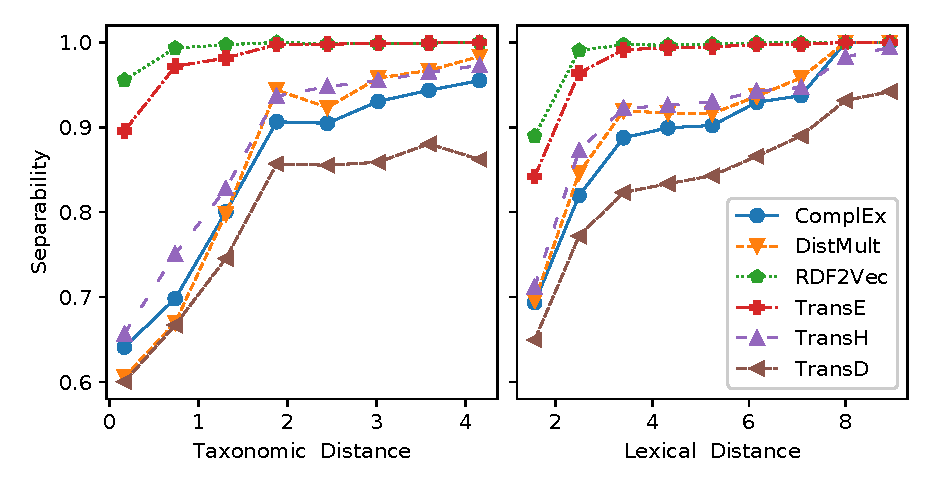
\includegraphics[width=\linewidth]{fig/plot/sep1_dist.eps}
  \caption{Séparabilité moyenne entre deux classes en fonction de leur distance taxonomique (à gauche) et de leur distance lexicale (à droite), pour différents modèles de plongement. }
  \label{fig:separability-lexical}
\end{figure}

\begin{figure}[h]
  \centering
  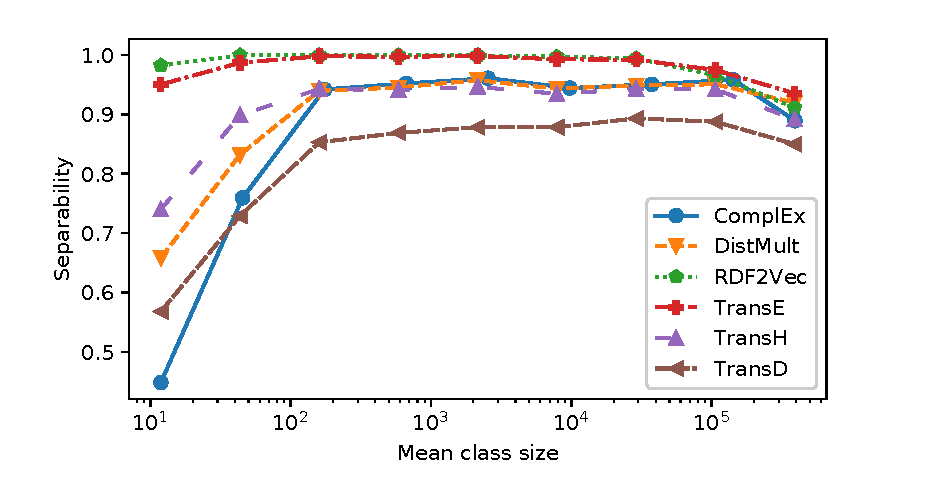
\includegraphics[width=\linewidth]{fig/plot/separability2_type1.eps}
  \caption{Séparabilité moyenne entre deux classes en fonction de la fréquence de ces classes, pour différents modèles de plongement.}
  \label{fig:separability-freq}
\end{figure}

Comme attendu, le score de séparabilité est dépendant de la distance lexicale et taxonomique entre les classes, et ce pour tous les modèles. Tous les modèles sauf TransD parviennent à séparer correctement les classes distantes (distance lexicale supérieur à 8, ou distance taxonomique supérieure à 3); en revanche, seuls deux modèles parviennent à conserver des scores élevés sur l'essentiel de l'intervalle : RDF2Vec et TransE, avec un avantage net pour RDF2Vec dans les faibles distances. La séparabilité moyenne de ces deux modèles diminue pour les classes très proches (distance taxonomique inférieure à 1, distance lexicale inférieure à 2), mais elle demeure supérieure à 85\%. Tous les autres modèles obtiennent des résultats nettement inférieurs.

Dans la figure \ref{fig:separability-freq}, on observe que les classes rares sont plus difficilement séparables que les classes fréquentes, quoique tous les modèles n'ont pas la même sensibilité à la fréquence : RDF2Vec et TransE n'ont qu'une légère baisse de score pour les classes rares (moins de $10^2$ instances en moyenne), qui peut partiellement être causée par le faible nombre d'échantillons sur lesquels entraîner la SVM. En revanche, les autres modèles ComplEx, DistMult, TransH et TransD y sont très sensibles. Cette sensibilité ne s'explique pas par une corrélation entre les paires rares et les paires proches, puisque les coefficients de Spearman et de Pearson entre les variables de distance et de fréquence sont proches de zéro.

%we observe that rare classes are indeed less separable than more frequent classes, with some variability depending on embedding models. RDF2Vec is once again the best model, with TransE slightly behind. TransH, DistMult and ComplEx have close scores in the size range $[200, 10^5]$, but ComplEx is more sensitive to rare classes than DistMult, which is itself more sensitive than TransH. More surprisingly, we observe that scores also decrease for very frequent classes (mean size above $10^5$ instances) for all embedding models. Both Pearson and Spearman’s correlations between lexical distance and mean class size are close to zero, which rules out the possibility of a bias in the dataset. An explanation is that frequent classes are more likely to be parent of other classes in the dataset (for example, \texttt{dbo:Agent} is the second most frequent class of the dataset, and is a parent of half the classes in the DBpedia ontology), and separating a subclass from its parent is harder than separating sibling or unrelated classes. Finally, we observe a convergence of scores for frequent classes between all models, with TransE achieving the highest score.

En résumé, seuls deux modèles obtiennent une mesure $F1$ moyenne supérieure à 95\% sur notre tâche de séparabilité : RDF2Vec et TransE, avec respectivement 99.7\% et 99?2\% respectivement. 
%\label{sec:kge-sep}
             % Premier thème (Doctorat) ou "Détails de la Solution" (Maîtrise).
\Chapter{EXTRACTION DE TAXONOMIE}\label{chap:te}

Comme expliqué en introduction \ldots


\section{Exposé du problème}
\subsection{Problème}
\label{sec:problem}
Soit $\KG \subseteq \Ent \times \Rel \times \Ent$ un graphe de connaissance. Pour une entité $e \in \Ent$, on dit que $e$ est de type $t$ si le triplet $(e, \texttt{rdf:type}, t)$ appartient à $\KG$. Dans la littérature, les types sont souvent appelés des \textit{classes} : ici, on préfère l'usage de \textit{type} pour éviter des conflits de notation avec les \textit{clusters}, qui seront introduits dans la section~\ref{subsec:clustering}. Notons qu'une entité peut avoir plusieurs types : ainsi, \dbr{Charles\_Baudelaire} est à la fois de type \dbo{Poet}, \dbo{Writer} et \dbo{Agent}.

On note $\cal{T}$ l'ensemble des types contenus dans le graphe. L'enjeu est de construire une taxonomie $T$ sur $\cal{T}$, c'est-à-dire un ensemble d'axiomes de subsumption $\{(t_i \sqsubseteq t_i')\}_{i=1, \ldots}$. Dans un axiome $t \sqsubseteq t'$, $t$ est appelé un \textit{sous-type} de $t'$, et $t'$ un \textit{supertype} de $t$; l'axiome signifie que $t'$ est un type plus général que $t$, et donc que tout élément de type $t$ est aussi de type $t'$. Pour être valide, une taxonomie $T$ doit vérifier une structure d'arbre, c'est-à-dire respecter deux conditions : chaque type doit avoir au plus un supertype, et $T$ ne doit pas contenir de cycle, donc ne doit contenir aucune séquence $t_0, t_1, \ldots, t_k$ telle que $t_0 \sqsubseteq t_1 \sqsubseteq \ldots \sqsubseteq t_k \sqsubseteq t_0$.

Comme données d'entraînement, on suppose avoir accès à un jeu de données $\cal{D} = \{ (\mathbf{e_i}, t_i) \}_{i=1, \ldots, N}$, constitué de $N$ paires $(\bf{e_i}, t_i) \in \R^d \times \cal{T}$ où $\bf{e_i}$ représente le plongement vectoriel de l'entité $e_i$, et $t_i$ son type. 

Pourquoi ?
extraire l'information taxonomique contenue dans la géométrie des plongements vectoriels
éviter d'exploiter des co-occurrences présentes dans les données, qui peuvent être causées par le fait que l'on a eu accès à une taxonomie lors de la création du graphe.

Relâcher cette contrainte : donne accès au graphe complet, et pas seulement aux embeddings + avoir accès aux co-occurences. Dans ce cas, beaucoup plus d'information = donne la possibilité d'extraire une taxonomie plus riche, cf chapitre suivant.

\subsection{Données}

DBpedia

\section{Méthode proposée}

Le préalable à notre méthode est le plongement du graphe dans $\R^d$. Pour cela, on s'appuie sur les travaux préliminaires décrits dans la section~\ref{chap:kge}.
Notre point de départ est donc une matrice de dimension $N \times d$, qui peut être vue comme un nuage de points dans $\R^d$.

\subsection{Regroupement hiérarchique}
\label{subsec:clustering}
La première étape consiste à exécuter un algorithme de regroupement (ou \textit{clustering}) hiérarchique agglomératif sur ce nuage de points. 
On commence avec $N$ clusters singletons, chacun contenant l'une des $N$ entités de départ. À chaque étape, deux des clusters existants sont fusionnés pour former un nouveau cluster. Les clusters à fusionner sont choisis de sorte à minimiser un certain critère : ce critère peut être la distance moyenne entre les entités des clusters, la distance minimale ou maximale entre ces entités, ou la variance du nouveau cluster. 
L'algorithme s'arrête lorsqu'il ne reste plus qu'un seul cluster qui contient toutes les entités; ce cluster est appelé cluster racine. Le résultat de cet algorithme est un arbre binaire, dont la racine est le cluster racine contenant toutes les entités, et dont les feuilles sont les $N$ clusters singletons.


On note $\Clusters$ l'ensemble des clusters, $X$ l'arbre de clustering obtenu, et $\texttt{racine}$ la racine de l'arbre – c'est-à-dire, le cluster contenant toutes les entités. On peut écrire $X = (V_X, E_X)$, avec $V_X = \Clusters$ l'ensemble des sommets de $X$, et $E_X = \{(C_i, C_i')\}_{i = 1, 2, \ldots } \subseteq \Clusters^2$ l'ensemble des arêtes de $X$.

Pour deux clusters $C$ et $C'$, on dit que $C$ est un prédecesseur de $C'$ si $C$ appartient à l'unique chemin entre la racine et $C'$, et on note $C \preceq C'$. Dans ce cas, on appelle $C'$ un successeur de $C$, noté $C' \succeq C$. De plus, on dit que $C$ est un prédecesseur \textit{strict} de $C'$ si $C$ est un prédecesseur de $C'$ avec $C \neq C'$. La relation $\prec$ définit un ordre partiel sur l'arbre $X$.

Pour un cluster $C$ donné, on définit $X[C]$ le sous-arbre de racine $C$ comme l'arbre contenant $C$ et tous ses successeurs:
\begin{equation}
    X[C] = (\{C' \in \Clusters : C' \succeq C\}, \{(C_1, C_2) \in E_X : C_2 \succ C_1 \succeq C\})
\end{equation}

Enfin, on définit $\gauche(C)$ et $\droite(C)$ respectivement les sous-clusters gauche et droit de $C$, et $\succs(C)$ l'ensemble des successeurs de $C$.


Considérations temportelles ? Complexité de l'algorithme ?

Étape non-supervisée


\subsection{Association type-cluster}
On a d'un côté, une hiérarchie sur des groupes d'entités (les clusters), de l'autre, une liste de types non hiérarchisé; but de l'étape : fusionner ces deux sources d'information, utiliser la structure sur les entités pour créer une structure sur les types. Pour cela, on injecte les types dans l'arbre de clustering, en associant chaque type à un cluster. Pour ce faire, deux méthdoes : 
- associer à chaque type un unique cluster
- définir, pour chaque type, une probabilité d'injection, ou un score d'association avec tous les clusters


\subsubsection{Méthode 1: \textit{Hard Mapping}}

Pour pouvoir associer les types aux clusters pertinents, il faut mesurer à quel point un cluster $C$ donné représente un type $t$. Pour ce faire, on peut utiliser la précision et le rappel de ce cluster pour $t$. Posons $N_{C,t} = | e \in C, type(e) = t|$ le nombre d'entités de type $t$ contenues dans le cluster $C$,
$N_t = |e \in \mathcal{D}, type(e) = t|$ le nombre d'entités de type $t$ dans l'ensemble des données, et $N_C = | C |$ le nombre total d'entitésd dans le cluster $C$. On peut alors définir la précision, le rappel et la mesure $F_1$ :
\begin{align}
    p(C, t) &= \frac{N_{C, t}}{N_C} \\
    r(C, t) &= \frac{N_{C, t}}{N_t} \\
    F(C, t) &= 2 \cdot \frac{p(C, t)r(C, t)}{p(C, t) + r(C, t)} = 2 \cdot \frac{N_{C,t}}{N_C + N_t}
\end{align}

La mesure $F_1$ varie entre 0 et 1: 0 indique que le cluster $C$ ne contient aucune entité de type $t$; 1 signifie que le cluster contient uniquement des entités de type $t$ et que toutes les entités de type $t$ sont contenues dans le cluster. 

Ideally, we would map type $t$ to the cluster that maximizes its F-score, \textit{i.e} choose $m^*(t) = \argmax_C F(C, t)$, but then we could have two types mapped to the same cluster. 
If two types $t_A$ and $t_B$ are mapped to the same cluster $C$, then any type that is mapped to a successor of $C$ will have both $t_A$ and $t_B$ as ancestors, and the resulting taxonomy will not be valid. The mapping thus need to be unambiguous. Formally, this condition means that we need to find a injective mapping between types and clusters $m^* : \mathcal{T} \rightarrow \mathcal{C}$, so that distinct types are mapped to distinct clusters.  

Idéalement, on souhaiterait associer chaque type $t$ au cluster qui maximise sa mesure $F_1$, et donc choisir $m^*(t) = \argmax_C F(C, t)$, mais on pourrait alors avoir deux types associés au même cluster. Or, si deux types $t_A$ et $t_B$ sont associés au même cluster $C$, alors tout type associé à un successeur de $C$ aurait à la fois $t_A$ et $t_B$ comme prédecesseurs, et la taxonomie résultante serait donc invalide, selon les conditions énoncées en section~\ref{sec:problem}. Il faut donc garantir une association univoque entre types et clusters. Formellement, cela signifie que la fonction d'association $m^* : \Types \rightarrow \Clusters$ entre les types et les clusters doit être injective :
\begin{equation}
    \forall t, t' \in \Types, t \neq t' \implies m^*(t) \neq m^*(t')
\end{equation}


Pour une injection $m : \Types \rightarrow \Clusters$, on définit un score $J(m)$ qui mesure la qualité de l'association type-cluster définie par $m$. Ce score est simplement la mesure $F_1$ globale induite par $m$ :
\begin{equation}
    J(m) = \sum_{t \in \mathcal{T}} F(m(t), t)
\end{equation}

Notre association optimale est alors :
\begin{equation}
    m^* = \argmax_{
\substack{m : \Types \rightarrow \Clusters \\ m\text{ injective}}} \sum_{t \in \mathcal{T}} F(m(t), t)
\label{eq:optim-mapping}
\end{equation}


L'équation~\ref{eq:optim-mapping} définit un problème d'affectation linéaire, pour lequel une solution optimale existe dans tous les cas (et est unique si les mesures $F_1$ sont uniques pour chaque cluster).
Cette solution optimal peut être trouvée par l'algorithme de Jonker-Volgenant, avec une complexité de $O(|\Clusters|^3)$ dans le pire des cas \cite{jonker1987shortest}. Toutefois, l'utilisation de l'heuristique \textit{Asymmetric Greedy Search} \cite{brown2017heuristic} permet de réduire cette complexité, tout en trouvant des solutions dont le score est supérieur à 99.9\% du score optimal, en moyenne.
%, which can be useful when the size of $\mathcal{D}$ increases.

\subsubsection{Méthode 2: \textit{Soft Mapping}}

L'approche précédente aboutit à une fonction de décision binaire : un axiome $(t_i \sqsubset t_j)$ est prédit ou non, sans intermédiaire possible. Ceci parce que la fonction $\argmax$ de l'équation~\ref{eq:optim-mapping} n'est pas continue. En conséquence, la taxonomie prédite est sensible à des légers changements dans les données d'entrée.

Dans cette version, on explore une version lissée de l'approche précédente : l'association entre types et clusters est conservée, mais elle est lissée en remplacant la fonction $\argmax$ par une fonction softmax. Ainsi, un type n'est plus associé à un unique cluster; on lui attribue plutôt un vecteur de probabilité qui mesure combien chaque cluster le répresente bien. Ensuite, comme précédemment, cette association type-cluster est utilisée pour transformer la hiérarchie des clusters en une hiérarchie des types. Par rapport au cas précédent, la condition d'injectivité de l'association disparaît : une étape supplémentaire est nécessaire pour transformer le graphe de subsumption en une taxonomie valide. Ainsi, la discontinuité identifiée précédemment ne disparaît pas, mais elle est déplacée : au lieu d'intervenir lors de l'extraction des axiomes de subsumption, elle apparaît lors de la création de la taxonomie prédite à partir de ces axiomes. 

La première étape est de transformer les mesures $F_1$ en probabilités, à l'aide d'une fonction softmax. Pour un type $t$ et un cluster $C$, on définit ainsi la probabilité que le cluster $C$ représente le type $t$ :
\begin{equation}
    P(m(t) = C) = \frac{\displaystyle e^{ \beta F(t, C)}}{\displaystyle \sum_{C' \in \mathcal{C}} e^{\beta F(t, C')}}
\end{equation}

Le paramètre $\beta > 0$ contrôle la concentration de la distribution autour du maximum. Le cas $\beta \rightarrow 0$ attribue à tous les axiomes la même probabilité, tandis que le cas $\beta \rightarrow \infty$ donne toute la masse de probabilité à la valeur maximum, ce qui se rapproche de l'approche précédente. Le choix de la valeur de $\beta$ est discuté dans la section 

Ce score d'injection $P(m(t) = C)$ peut ensuite être utilisé pour calculer la probabilité d'un axiome de subsumption $(t' \sqsubset t)$, en tirant profit de la structure d'arbre qui existe entre les clusters. 
Écrire ce score d'injection comme une probabilité $P(m(t) = C)$ permet d'interpréter $(m(t) = C)$ comme un événement aléatoire, et donc $m(t)$ comme une variable aléatoire. On peut donc envisager l'approche de la façon suivante : le type $t$ est localisé quelque part dans l'arbre de clustering, mais cette localisation est entachée d'incertitude, ce que modélise la variable aléatoire $m(t)$. Par définition du softmax, la position la plus probable de $t$ est le cluster qui a le score $F_1$ le plus élevé; toutefois, là où la méthode du hard mapping ne considérait pas d'autre possibilité, d'autres positions de $t$ sont possibles. 

Dès lors, l'axiome $(t' \sqsubset t)$ est lui aussi un événément aléatoire. Cet événement se réalise si, dans l'arbre, \ldots

Note : une idée : et si on notais $Z_t$ la variable aléatoire correspondant à $m(t)$ ? Ça simplifierais peut etre les notations et la compréhension de la méthode. $m(t)$ c'est pas clair ce que ça représente, alors que $Z_t$ ça représente le cluster associé à $t$ (comme dans le hard mapping), sauf qu'on ne sait pas ù est $Z_t$. Intro : «on modélise la situation> (comme c'est une modélisation on est plus comptables de la véracité de nos hypothèses, notamment l'indepndance des $Z_t$)

On définit un score d'association $\sigma(t, C)$:
\begin{equation}
    \sigma(t, C) = \frac{\displaystyle e^{ \beta F(t, C)}}{\displaystyle \sum_{C' \in \mathcal{C}} e^{\beta F(t, C')}}
\end{equation}

On définit une famille de variables aléatoire $\cal{Z} = (Z_t)_{t \in \Types}$, indépendantes et à valeur dans $\Clusters$. Pour un type $t$ donné, la loi de la variable $Z_t$ est donné par :
\begin{equation}
    P(Z_t = C) = \sigma(t, C)
\end{equation}
On interprète la variable aléatoire $Z_t$ comme le cluster associé à $t$ dans l'arbre de clustering. Contrairement au cas précédent, où on aurait eu $Z_t = \argmax_C F(C, t)$ (à la condition d'injectivité près), ici on accepte que l'associé de $t$ soit incertain. \todo{Justifier l'indépendance}

Dès lors, on peut interpréter l'événement $t' \sqsubset t$ comme l'événement $Z_t \prec Z_{t'}$, et donc, en utilisant l'indépendances des $Z_t$ : 
\begin{align}
    \label{eq:softmapping_2}
    P(t' \sqsubset t) &= P(Z_t \prec Z_{t'}) \\
    &= \sum_{\substack{C_A, C_B \in \mathcal{C} \\ C_A \prec C_B}} P(Z_{t }= C_A, Z_{t'} = C_B) \nonumber \\
    &= \sum_{\substack{C_A, C_B \in \mathcal{C} \\ C_A \prec C_B}} P(Z_{t }= C_A)\cdot P(Z_{t'} = C_B)
\end{align}

Pour calculer ces probabilités pour chaque $t, t'$ sans sommer sur toutes les paires de clusters, on peut concevoir un algorithme récursif de type «diviser pour régner». Pour cela, il nous faut exprimer $P(t' \sqsubset t)$ sous forme récursive. On introduit donc une nouvelle quantité,  $P_C(t' \sqsubset t)$ : c'est, comme dans l'équation~\ref{eq:softmapping_2}, la probabilité de l'événement $t' \sqsubset t$ (c'est-à-dire de l'événément $Z_t \prec Z_{t'}$), mais restreint au cas où $Z_t$ et $Z_{t'}$ appartienent au sous-arbre $X[C]$. Or appartenir au sous-arbre $X[C]$ est équivalent à être un successeur de $C$, on peut donc réécrire l'événement $(Z_t \prec Z_{t'}) \land (Z_t, Z_{t'} \in X[C])$ sous la forme $C \preceq Z_t \prec Z_{t'}$. D'où :
\begin{align}
    P_C(t' \sqsubset t) &= P(C \preceq Z_t \prec Z_{t'}) \nonumber \\
    &= \sum_{\substack{C_A, C_B \in \succs(C) \\  C_A \prec C_B}} P(Z_t = C_A)\cdot P(Z_{t'} = C_B) \label{eq:proba_subsumption}
\end{align}


% To compute these probabilities for all $t, t'$ without summing over all pairs of % clusters, we devise a divide-and-conquer algorithm. For this, we need a recursive % formulation of $P(t' \sqsubset t)$, so we introduce $P_C(t' \sqsubset t)$, the % probability of axiom $(t' \sqsubset t)$ computed on the subtree $X[C]$, for any given % cluster $C$. Similarly to equation~\ref{eq:softmapping_2}, it represents the % probability that the cluster $m(t)$ representing $t$ is a predecessor of  the cluster % $m(t')$ representing $t'$, with the additional condition that both $m(t)$ and $m(t')$ % must belong to the subtree $X[C]$ (that is, be successors of $C$):
% \begin{align}
%     P_C(t' \sqsubset t) &= P(C \preceq m(t) \prec m(t') % \text{ and } m(t),m(t') % \succeq C %, C \preceq m(t')
%     ) \nonumber \\
%     &= \sum_{\substack{C_A, C_B \in \succs(C) \\ C_A \prec C_B}} P(m(t) = C_A)\cdot % P(m(t') = C_B) 
%     \label{eq:proba_subsumption}
% \end{align}

Comme le sous-arbre $X[\texttt{racine}]$ est égal à l'arbre complet, on a $P_\texttt{racine}(t' \sqsubset t) = P(t' \sqsubset)$. Si on parvient à exprimer $P_\texttt{racine}$ en fonction de $P_{\gauche(\texttt{racine})}$ et de $P_{\gauche(\texttt{racine})}$

\ldots 

Soit $L = \gauche(C)$ et $R = \droite(C)$ les sous-clusters gauche et droit de $C$. On peut remarquer qu'un successeur de $C$ est soit un successeur de $L$, soit un successeur de $R$, soit $C$ lui-même. Autrement dit, en notant $\sqcup$ l'union disjointe :
\begin{equation}
    \succs(C) = \succs(L) \sqcup \succs(R) \sqcup \{ C\}
\end{equation}
En suivant cette observation, on peut donc partager la somme~\ref{eq:proba_subsumption} en trois :
\begin{align}
P_{C}(t' \sqsubset t) = 
&
\sum_{\substack{C_A, C_B \in \succs(L) \\  C_A \prec C_B}} P(Z_t = C_A)\cdot P(Z_{t'} = C_B) 
\nonumber \\ 
&+ 
\sum_{\substack{C_A, C_B \in \succs(R) \\  C_A \prec C_B}} P(Z_t = C_A)\cdot P(Z_{t'} = C_B) 
\nonumber \\
&+ \displaystyle \sum_{C_B \colon C \prec C_B} P(Z_t = C) \cdot P(Z_{t'} = C_B) \nonumber \\
= {} & P_{L}(t' \sqsubset t) + P_{R}(t' \sqsubset t)  + P(Z_t=C)\cdot\sum_{\substack{C_B \colon \\ C\prec C_B}} P(Z_{t'} = C_B)
\label{eq:proba_over_subtree}
\end{align}

Cette équation fait apparaître le lien recherché entre $P_C$ d'un côté, et $P_L$ et $P_R$ de l'autre. On l'écrire de façon plus concise sous forme matricielle. Pour cela, définissons $n_T = | \mathcal{T} |$ le nombre de types distincts, $\mathbf{Q_C}$ une matrice de dimension $n_T \times n_T$ telle que sa coordonnée $(i, j)$ contienne $P_C(t_j \sqsubset t_i)$, et $\mathbf{p_C} = \left(P(Z_{t_i} = C)\right)_{i = 1, \ldots, n_T}$ le vecteur de probabilité du cluster $C$, de dimension $n_T$. 

Avec ces notations, notre objectif est de calculer $\bf{Q_\texttt{racine}}$, et donc d'obtenir une formule récursive reliant $\bf{Q_C}$ à $\bf{Q_L}$ et $\bf{Q_R}$. L'équation \ref{eq:proba_over_subtree} se réécrit :
\begin{align}
    \mathbf{Q_C} &= \mathbf{Q_L} + \mathbf{Q_R} + \mathbf{p_C} \cdot \left(\sum_{C' \colon C \prec C'} \mathbf{p_{C'}} \right)^\top 
    \label{eq:recursive_q_formula}
\end{align}

À ce stade, l'équation \ref{eq:recursive_q_formula} est proche de la formulation récursive cherchée, mais il reste encore à éliminer la somme $\sum_{C' \colon C \prec C'} \mathbf{p_{C'}}$, parce qu'elle dépend de tous les successeurs stricts de $C$, et pas seulement de $C, L$ ou $R$. On note donc $\bf{s_C}$ cette somme :
\begin{align}
    \bf{s_C} &= \sum_{C' \colon C \prec C'} \mathbf{p_{C'}} \nonumber \\
            &= \sum_{C' \in \succs(C)^*} \mathbf{p_{C'}}
\end{align}
Cette somme est un vecteur de dimension $n_T$; sa $i$-ème coordonnée représente la probabilité pour le type $t_i$ d'être associé à un successeur strict de $C$, c'est-à-dire $P(Z_{t_i} \succ C)$. Or un successeur strict de $C$ est soit $L$ ou $R$, soit un successeur strict de $L$ ou $R$, ce qui s'exprime mathématiquement par :
\begin{equation}
    \succs(C)^* = \{L\} \sqcup \{R\} \sqcup \succs(L)^* \sqcup \succs(R)^*
\end{equation}

On peut donc réécrire $\bf{s_C}$ comme :
\begin{align}
    \mathbf{s_C} &= \mathbf{p_L} + \mathbf{p_R} + (\mathbf{s_L} + \mathbf{s_R}) \nonumber  \\
     &= (\mathbf{p_L}  + (\mathbf{s_L}) + (\mathbf{p_R} + \mathbf{s_R})
    \label{eq:l_def}
\end{align}
Finalement, on définit la probabilité pour chaque type d'être associé à un successeur non-strict de $C$ : 
\begin{equation}
    \mathbf{u_C} = \mathbf{p_C} + \mathbf{s_C}
    \label{eq:def_uc}
\end{equation}
Cela permet de reformuler ainsi l'équation \ref{eq:l_def}:
\begin{equation}
    \mathbf{s_C} = \mathbf{u_L} + \mathbf{u_R}
    \label{eq:l_update}
\end{equation}

On a désormais nos équations de récurrences : \ref{eq:recursive_q_formula} pour $\bf{Q_C}$, \ref{eq:def_uc} pour $\bf{u_C}$ et \ref{eq:l_update} pour $\bf{s_C}$. Il reste à calculer les cas de base, c'est-à-dire les valeurs de $\bf{Q, u, s}$ pour les clusters feuilles. Si $C$ est une feuille, la probabilité pour un type $t$ d'être associé à un de ses successeurs stricts est nulle, puisque $C$ n'a aucun successeur strict. Pour la même raison, la probabilité pour qu'un axiome de subsumption $t' \sqsubset t$ soit vérifié dans le sous-arbre $X[C]$ est également zéro. Ainsi $\mathbf{s_C}$ et $\mathbf{Q_C}$ sont respectivement nuls pour chaque cluster feuille. Quant à $\bf{u_C}$, sa valeur sur les feuilles peut être calculée par l'équation \ref{eq:def_uc}.

On peut finalement écrire les équations de récurrence pour $\mathbf{s_C}, \mathbf{Q_C}, \mathbf{u_C}$:
\begin{align}
    \mathbf{Q_C} &=
    \begin{cases}
      \mathbf{0}_{n_T,n_T} & \text{si $C$ est une feuille}\\
      \mathbf{p_C} \cdot \mathbf{s_C}^\top + \mathbf{Q_\text{left$(C)$}} + \mathbf{Q_\text{right$(C)$}} & \text{sinon}
    \end{cases}  \\
  \mathbf{s_C} &=
    \begin{cases}
      \mathbf{0}_{n_T} & \text{si $C$ est une feuille}\\
      \mathbf{u_\text{left$(C)$}} + \mathbf{u_\text{right$(C)$}} & \text{sinon}
    \end{cases}  \\
    \mathbf{u_C} &= \mathbf{p_C} + \mathbf{s_C}
\end{align}

Our implementation uses linear programming. We denote $D_C = (\mathbf{s_C}, \mathbf{Q_C}, \mathbf{u_C})$. Clusters are iterated over in a reverse DFS order. For each cluster $C$, we compute and cache $D_C$ using $D_{\text{left}(C)}$ and $D_{\text{right}(C)}$. The reverse DFS order guarantees that all successors of $C$ have already been visited, so $D_{\text{left}(C)}$ and $D_{\text{right}(C)}$ are already cached. After computing $D_C$, we can delete cached values $D_{\text{left}(C)}$ and $D_{\text{right}(C)}$ because no further computation depends on them. The last visited cluster is $\texttt{root}$: when the algorithm ends, the cache contains only $D_\texttt{root} = (\mathbf{s_\texttt{root}}, \mathbf{Q_\texttt{root}}, \mathbf{u_\texttt{root}})$, and the final probability matrix $\mathbf{Q_\texttt{root}}$ can be returned. Its $(i, j)$ coordinate contains the probability of axiom $(t_j \sqsubset t_i)$.
For a balanced binary tree, this algorithm guarantees a maximum cache size of $O(|\mathcal{T}|^2 \log_2(| \mathcal{C} |))$, with $|\mathcal{T}| \ll | \mathcal{C} |$.


\subsection{Construction de la taxonomie}

\section{Évaluation et discussion}
\subsection{Méthode d'évaluation}
\subsection{Résultats}

\begin{table}
    \centering
    \caption{
    Évaluation de notre approche et de TIEmb sur \textsc{DBpedia-Freq}, pour différents modèles de plongement. $p, r, F1$ désignent respectivement la précision, le rappel et la mesure $F1$. \textit{cos} et \textit{euc} indiquent les distances cosinus et euclidienne. Les résultats de la section \textit{Moyenne} sont obtenus en calculant la moyenne des évaluations directe et transitive.}
    \begin{tabular}{|lll|ccc|ccc|ccc|}
    \hline 
                               &      &          & \multicolumn{3}{c|}{Directe}              & \multicolumn{3}{c|}{Transitive}     & \multicolumn{3}{c|}{Moyenne}     \\
        Méthode	&	Plongements	&	Distance	&	$p$	&	$r$	&	$F$	&	$p$	&	$r$	&	$F1$	&	$p$	&	$r$	&	$F1$	\\	
\hline \multirow{8}{*}{TIEmb}	&	\multirow{2}{*}{ComplEx}	&	cos	&	0.38	&	0.38	&	0.38	&	0.28	&	0.57	&	0.37	&	0.33	&	0.48	&	0.38	\\
	&		&	euc	&	0.39	&	0.42	&	0.4	&	0.34	&	0.8	&	0.48	&	0.37	&	0.61	&	0.44	\\[2pt] 
	&	\multirow{2}{*}{DistMult}	&	cos	&	0.26	&	0.27	&	0.26	&	0.19	&	0.44	&	0.27	&	0.23	&	0.36	&	0.27	\\
	&		&	euc	&	0.37	&	0.41	&	0.39	&	0.33	&	0.79	&	0.47	&	0.35	&	0.60	&	0.43	\\[2pt] 
	&	\multirow{2}{*}{RDF2Vec}	&	cos	&	0.77	&	\textbf{0.84}	&	0.81	&	0.43	&	0.87	&	0.57	&	0.60	&	0.86	&	0.69	\\
	&		&	euc	&	0.70	&	0.77	&	0.73	&	0.30	&	0.73	&	0.42	&	0.50	&	0.75	&	0.58	\\[2pt] 
	&	\multirow{2}{*}{TransE}	&	cos	&	0.77	&	0.72	&	0.74	&	0.83	&	0.89	&	0.86	&	0.80	&	0.81	&	0.80	\\
	&		&	euc	&	0.76	&	0.75	&	0.76	&	0.7	&	0.9	&	0.79	&	0.73	&	0.83	&	0.78	\\[2pt] 
\hline \multirow{8}{*}{\shortstack[c]{Hard Mapping \\ (HM)}}	&	\multirow{2}{*}{ComplEx}	&	cos	&	0.53	&	0.5	&	0.52	&	0.78	&	0.7	&	0.74	&	0.66	&	0.60	&	0.63	\\
	&		&	euc	&	0.51	&	0.44	&	0.47	&	0.87	&	0.52	&	0.65	&	0.69	&	0.48	&	0.56	\\[2pt] 
	&	\multirow{2}{*}{DistMult}	&	cos	&	0.55	&	0.47	&	0.5	&	0.73	&	0.57	&	0.64	&	0.64	&	0.52	&	0.57	\\
	&		&	euc	&	0.43	&	0.36	&	0.39	&	0.75	&	0.54	&	0.63	&	0.59	&	0.45	&	0.51	\\[2pt] 
	&	\multirow{2}{*}{RDF2Vec}	&	cos	&	0.60	&	0.44	&	0.50	&	0.88	&	0.50	&	0.63	&	0.74	&	0.47	&	0.57	\\
	&		&	euc	&	0.60	&	0.53	&	0.56	&	0.89	&	0.64	&	0.74	&	0.74	&	0.58	&	0.65	\\[2pt] 
	&	\multirow{2}{*}{TransE}	&	cos	&	0.82	&	0.8	&	0.81	&	0.97	&	0.89	&	\textbf{0.93}	&	\textbf{0.90}	&	0.85	&	0.87	\\
	&		&	euc	&	0.73	&	0.67	&	0.7	&	\textbf{0.99}	&	0.68	&	0.8	&	0.86	&	0.68	&	0.75	\\[2pt] 
\hline \multirow{8}{*}{\shortstack[c]{Soft Mapping \\ (SM)}}	&	\multirow{2}{*}{ComplEx}	&	cos	&	0.52	&	0.48	&	0.5	&	0.89	&	0.7	&	0.79	&	0.71	&	0.59	&	0.65	\\
	&		&	euc	&	0.51	&	0.44	&	0.47	&	0.84	&	0.6	&	0.7	&	0.68	&	0.52	&	0.59	\\[2pt] 
	&	\multirow{2}{*}{DistMult}	&	cos	&	0.5	&	0.44	&	0.47	&	0.87	&	0.65	&	0.74	&	0.69	&	0.55	&	0.61	\\
	&		&	euc	&	0.48	&	0.42	&	0.45	&	0.86	&	0.65	&	0.74	&	0.67	&	0.54	&	0.60	\\[2pt] 
	&	\multirow{2}{*}{TransE}	&	cos	&	\textbf{0.83}	&	0.81	&	\textbf{0.82}	&	0.93	&	\textbf{0.93}	&	\textbf{0.93}	&	0.88	&	\textbf{0.87}	&	\textbf{0.88}	\\
	&		&	euc	&	0.78	&	0.77	&	0.77	&	0.98	&	0.87	&	0.92	&	0.88	&	0.82	&	0.85	\\[2pt] 
\hline
    \end{tabular}
    \label{tab:te-results}
\end{table}


\subsection{Discussion}

\section{Hyperparamètres}
\label{sec:hp}
\subsection{Base \texorpdfstring{$\beta$}{beta} du softmax}
\label{subsec:hp-beta}

\begin{figure}
    \centering
    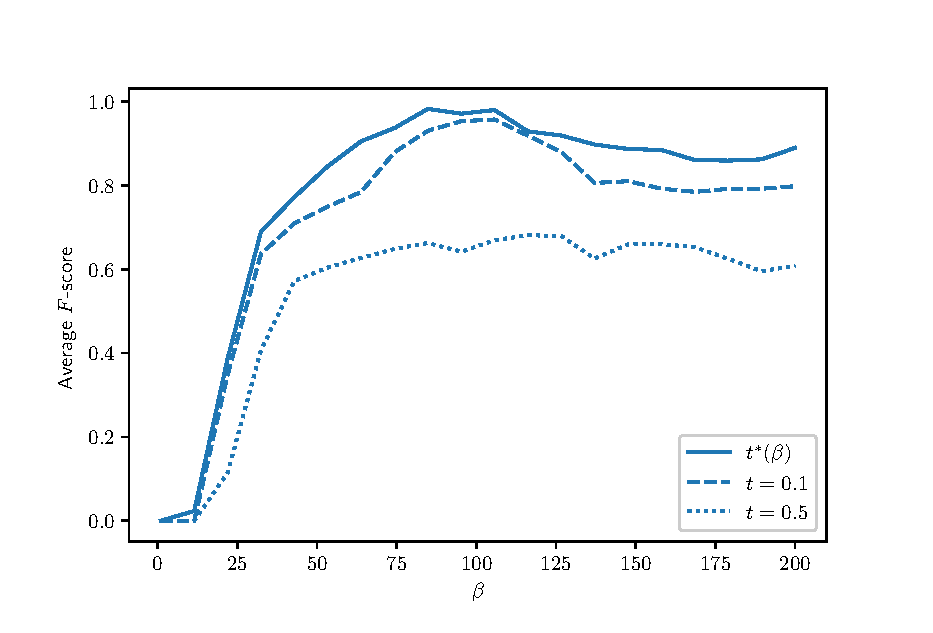
\includegraphics{fig/plot/average_beta_vs_best.eps}
    \caption{Taxonomy extraction $F$-scores obtained for different values of parameter $\beta$, with the optimal threshold $t^*(\beta)$ and two fixed threshold $0.1$ and $0.5$. Scores are averaged over five different subtaxonomies of DBpedia, and expressed as a fraction of the optimal score.}
    \label{fig:beta-search-1}
\end{figure}

\begin{figure}
    \centering
    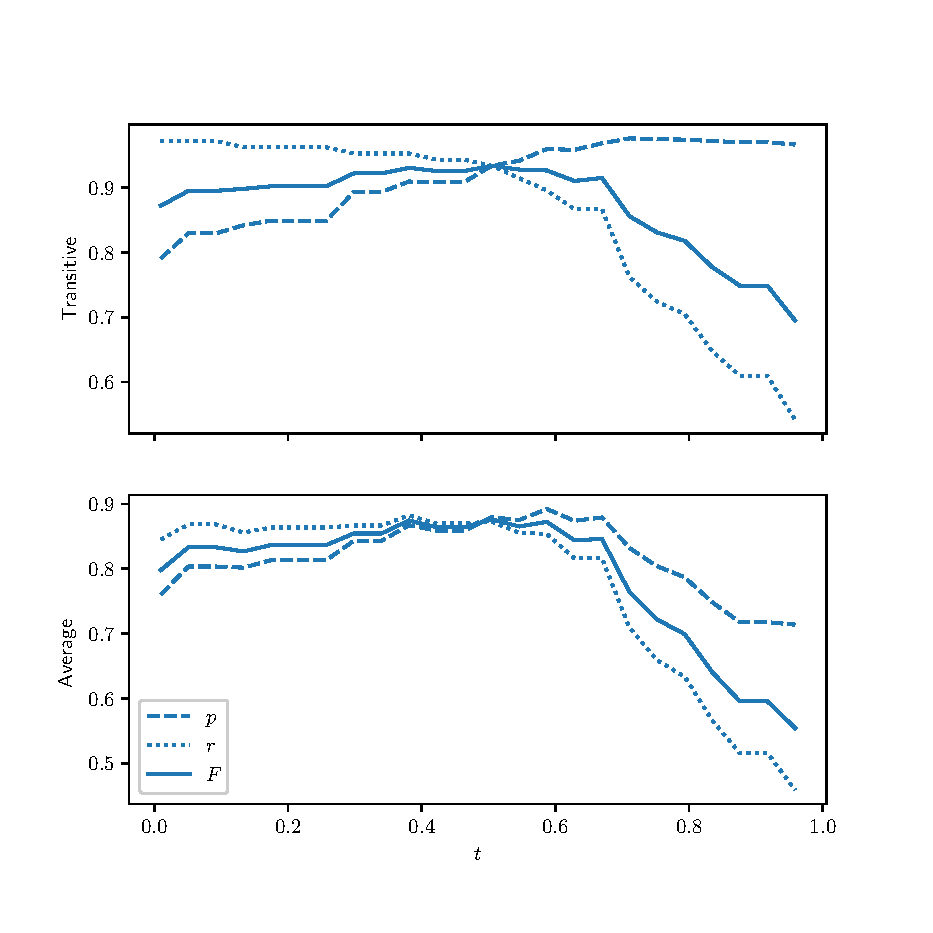
\includegraphics{fig/plot/threshold_exp.eps}
    \caption{Taxonomy extraction $F$-scores obtained for different values of parameter $\beta$, with the optimal threshold $t^*(\beta)$ and two fixed threshold $0.1$ and $0.5$. Scores are averaged over five different subtaxonomies of DBpedia, and expressed as a fraction of the optimal score.}
    \label{fig:beta-search-2}
\end{figure}

\begin{figure}
    \centering
    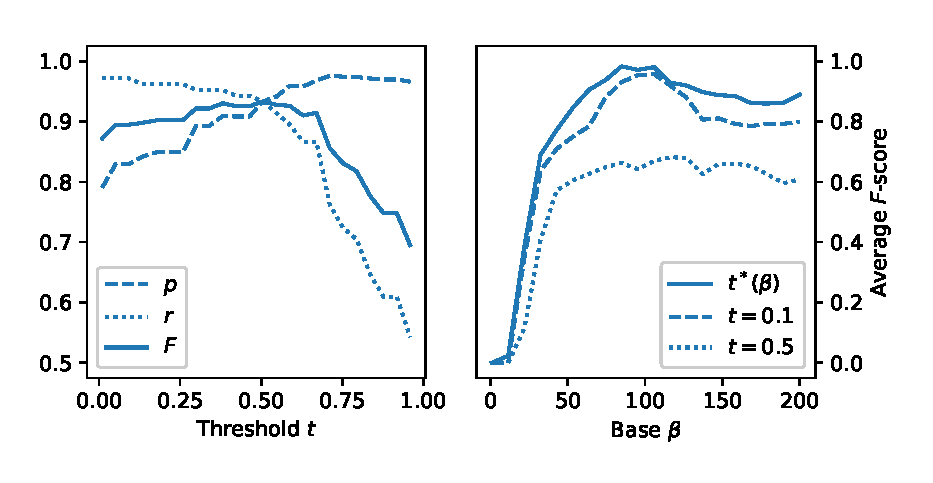
\includegraphics[width=\textwidth]{fig/plot/hp_results.eps}
    \caption{Influence des hyperparamètres $t$ et $\beta$ pour la méthode «soft mapping». À gauche, la précision, rappel et mesure $F1$ obtenus par évaluation transitive pour différentes valeurs de $t$ dans $[0, 1]$, et $\beta = 100$. À droite, les mesures $F1$ obtenues pour différentes valeurs du paramètre $\beta$, et pour trois différents seuils : le seuil optimal $t^*(\beta)$ et deux seuils fixes $t=0,1$ et $t=0,5$. Les scores affichés sont obtenus en moyennant les résultats obtenus sur cinq sous-taxonomies de DBpedia, et exprimées comme une fraction du score optimal.
    }
    \label{fig:t-search-1}
\end{figure}
\label{subsec:hpsearch}             % Second thème (Doctorat) ou "Résultats théoriques et expérimentaux" (Maîtrise).
\Chapter{EXTRACTION DE TAXONOMIE EXPRESSIVE}
\label{chap:texp}

\section{Motivation et principes généraux}

Dans la section précédente, on a décrit une méthode pour extraire une hiérarchie entre les types à partir des seuls plongements d'entité. 

Méthode précédente : on s'interdit d'utiliser le linked data => comment retrouver l'information connue (la taxonomie DBpédia) à partir des seuls plongements vectoriels ?

Cette méthode : en utilisant toute l'information accessible, comment aller plus loin que ce qui existe (en l'occurence, trouver une taxonomie expressive – qui à l'heure actuelle n'existe pas)

Pas d'utilisation du Linked Data = méthode très descriptive, qui n'utilise pas toute l'information à notre disposition.

Schéma général proche de la méthode précédente : regroupement hiérarchique sur les entités, puis transformation de la hiérarchie entre entités en une hiérarchie sur les classes. Ici, étiquettage de la classe plus sophistiqué, puisuq'on s'autorise Linked Data

Pourquoi ça marche ? Parce qu'on travaille sur un groupe d'entités dont on sait qu'elles sont sémantiquement proches, de par la géométrie de leurs plongements. Donc on restreint la dimension de l'espace de recherche, qui est un goulot d'étranglement habituel des méthodes d'extraction d'axiomes.

Toutefois, un ajout majeur : le retirage récursif des entités à regrouper pour limiter la propagation des erreurs dans l'arbre, limiter le bruit et affiner progressivement la spécificité des classes extraites. Plus un \textit{bag of tricks} pour que ça marche bien.

\paragraph{Remarque}

DBpédia, comme la plupart des graphes de connaissances, fonctionne sous l'hypothèse du monde ouvert : si un triplet est absent du graphe, cela ne signifie pas nécessairement qu'il est faux. Aussi, dans la suite, lorsqu'on écrit qu'une entité $x$ ne vérifie pas un prédicat logique $P$, cela doit être compris comme un raccourci pour écrire que l'assertion $P(x)$ n'est pas contenue dans le graphe, et non comme l'assertion $\neg P(x)$.

\section{Méthode proposée}
\subsection{Regroupement hiérarchique récursif avec retirage}

La méthode d'extraction de taxonomie expressive commence elle aussi par une phase de regroupement hiérarchique. Dans la méthode précédente, on avait comme seules données d'entrée un ensemble fixé d'entités typées $\cal{D}$. Ici au contraire, on s'autorise l'accès à tout le graphe, donc l'ensemble $\cal{D}$ sur lequel s'opère le regroupement hiérarchique est variable et change au cours de l'exécution de l'algorithme. À chaque étape $t$, on effectue un regroupement hiérarchique sur les plongements des entités de $\cal{D}_t$, puis on étiquette les clusters obtenus avec des axiomes logiques (l'extraction d'axiomes à partir de clusters est détaillée dans la section \ref{subsec:texp-exaxiom}). Chaque nouvel axiome extrait sert alors à créer un nouveau jeu de données, sur lequel on répète l'étape précédente, ce qui permet d'étendre itérativement la taxonomie prédite.

% Ensuite, pour chacun des axiomes $a_1, \ldots, a_k$ obtenus, on tire aléatoirement des entités qui vérifient cet axiome, ce qui donne de nouveaux ensembles d'entrées $\cal{D}_{t+1}, \ldots, \cal{D}_{t+k}$.

Dans cette section, on se donne une fonction d'extraction d'axiome $\alpha$, telle que $\alpha(C)$ est un axiome logique qui qualifie le cluster $C$, si un tel axiome existe, et qui renvoie un symbole spéciale \texttt{indéfini} dans le cas contraire. Un exemple d'une telle fonction est donné dans la section suivante. 

% Principe général
On dispose d'une file d'axiomes à traiter $A$, et de la taxonomie en cours de construction $\Tpred$. La file d'axiomes à traiter n'est autre que la liste des feuilles de $\Tpred$ qui n'ont pas encore été visitées. Lorsqu'on visite un axiome $\alpha$ de $A$, soit on parvient à extraire un sous-arbre $T_\alpha$ qui contient des axiomes, et alors $T_\alpha$ est ajouté à $\Tpred$ à l'emplacement de $\alpha$, et les nœuds feuilles de $T_\alpha$ sont ajoutés à la file des axiomes à traiter; soit on ne trouve aucun sous-axiome pertinent pour $\alpha$, auquel cas $\alpha$ reste une feuille de $\Tpred$ et la recherche continue dans les autres axiomes de la file $A$, jusqu'à épuisement de $A$.

Pour la première étape, $A$ est initialisée à $\{\top\}$ : le seul axiome de $A$ est le concept universel $\top$ qui, par définition, est vérifié par toutes les entités du graphe. $\top$ sert de racine à la taxonomie, puisque c'est le seul axiome dont on soit sûr \textit{a priori} qu'il définisse toutes les entités.
La taxonomie $\Tpred$ est réduite à un seul sommet $\top$ et ne contient donc aucune arête. 

Tant que la file $A$ n'est pas vide, on retire son premier élément $a$, qui sert d'axiome d'entrée pour cette étape. On prélève aléatoirement, dans le graphe $\KG$, $N$ entités parmi celles qui vérifient $a$ – dans notre implémentation, le graphe est représenté \textit{via} une librairie Python spécifique, mais dans d'autres contextes, le langage de requête SPARQL pourrait être utilisé à cette fin. Les plongements de ces entités donne un nuage de points $\cal{D}_a$ de dimension $d \times N$, avec $d$ la dimension des entités.

Sur ce nuage de point $\cal{D}_a$, on effectue un regroupement hiérarchique, comme décrit dans la section \ref{subsec:te-clustering}. À nouveau, on considère deux choix de paramètres de cet algorithmes : distance euclidienne avec critère de Ward, et distance cosinus avec liaison moyenne. La première fusionne les clusters de façon à minimiser la variance du nouveau cluster créé. À l'étape $t$, notons $\cal{C}_t$ les clusters existant; les clusters $C_1$ et $C_2$ à fusionner sont choisis selon l'équation :
\begin{equation}
    C_1, C_2 = \argmin_{C_1, C_2 \in \cal{C}_t} 
    \frac{1}{| C_1 + C_2 |} \sum_{\bf{e} \in C_1 \cup C_2} \| \bf{e} - \frac{1}{| C_1 + C_2 |} \sum_{\bf{e'} \in C_1 \cup C_2} \bf{e'} \|_2^2 
\end{equation}
La seconde fusionne les clusters dont les entités ont la distance moyenne la plus faible. On fusionnera donc $C_1$ et $C_2$ tels que :
\begin{equation}
    C_1, C_2 = \argmin_{C_1, C_2 \in \cal{C}_t} \frac{1}{|C_1| \times |C_2|} \sum_{\bf{e_1}\in C_1} \sum_{\bf{e_2} \in C_2} d_\text{cos}(\bf{e_1, e_2})
\end{equation}

Le résultat est un arbre binaire, noté $X_a$, dont la racine est $\cal{D}_a$ tout entier, et dont les feuilles sont les $N$ éléments de $\cal{D}_a$. 

On effectue alors un parcours de l'arbre $X_a$, en excluant la racine $a$ qui est déjà étiquettée : pour un cluster $C$, on calcule $\alpha(C)$ pour trouver l'axiome associé à $C$. Si $\alpha(C) = \texttt{indéfini}$, le cluster $C$ n'a pas de signification logique accessible, et on poursuit la recherche dans les sous-clusters. Au contraire, si $\alpha(C)$ existe, on interrompt la recherche, et on ajoute $\alpha(C)$ à la file d'axiomes à visiter. Au-delà d'une certaine profondeur $D_\text{max}$ dans l'arbre, on arrête la recherche. On note $L_\alpha(a)$ l'ensemble des cluster $C$ étiquettés rencontrés lors de la recherche.

Finalement, on construit la sous-taxonomie extraite $T_a$ à partir de $X_a$ en suivant la procédure décrite à la section \ref{subsec:te-taxconstruction} : $T_a$ ne contient que les sommets de $X_a$ qui sont étiquettés, et qui laisse la relation de succession entre clusters inchangée :
\begin{align}
    T_a = (&\{C \in X_a : \alpha(C) \neq \texttt{indéfini}\}, \nonumber \\
    &\{(C, C' \in X_a : \exists C_1, \ldots, C_k \in X_a, \alpha(C_1) = \ldots = \alpha(C_k) = \texttt{indéfini} \nonumber \\
    &\text{ et } C \prec C_1 \prec \ldots \prec C_k \prec C'\})
\end{align}
Autre formulation\todo{choisir entre les deux notations} :
\begin{align}
    T_a = (L_\alpha(a), \nonumber 
    \{(C, C' \in X_a : \exists C_1, \ldots, C_k \in X_a \setminus L_\alpha(a), C \prec C_1 \prec \ldots \prec C_k \prec C'\})
\end{align}

Enfin, si au moins l'une des feuilles de $X_a$ n'est pas couverte par un axiome $\alpha(C)$, c'est-à-dire s'il existe au moins une branche allant des feuilles à la racine qui ne contient pas d'étiquette, c'est qu'une partie de l'arbre n'a pas été décrite par un axiome, et qu'il reste potentiellement de nouveaux axiomes à extraire. Dans ce cas, un nœud spécial \texttt{<?>} est ajouté à $T_a$ et relié directement à $a$. La signification logique de ce nœud s'écrit :
\begin{equation}
    \texttt{<?>} = a \land \left( \bigwedge\limits_{C \in L_\alpha(a)} \neg \alpha(C) \right)
    \label{eq:texp-special-node}
\end{equation}
Soit, en langage courant, l'ensemble des éléments qui vérifient $a$ mais ne vérifient aucun des sous-axiomes $\alpha(C)$ de $a$. Cette définition purement négative n'est pas d'une grande utilité dans une taxonomie expressive, puisqu'elle exprime simplement la tautologie $C \sqsubset \neg C = \top$. On utilise donc le symbole \texttt{<?>} pour signifier que la recherche n'est pas encore finie pour $a$ et qu'il reste des sous-axiomes de $a$ à trouver.

Si $T_a = (\varnothing, \varnothing)$, c'est-à-dire qu'aucun axiome n'a été trouvé en parcourant l'arbre $X_a$, alors $a$ n'aura pas de sous-axiome dans la taxonomie extraite et restera une feuille de $\Tpred$. Sinon, on remplace le nœud $a$ de $\Tpred$ par la sous-taxonomie $T_a$. On répète alors l'étape précédente, tant que la file d'axiomes $A$ n'est pas vide.

\paragraph{Le cas des nœuds spéciaux \texttt{<?>}} Dans l'étape précédente, le cas où l'axiome de départ $a$ est l'axiome spécial \texttt{<?>} est traité un peu différemment du cas général. Les données d'entrées sont toujours tirées aléatoirement, suivant la formule \ref{eq:texp-special-node}; le regroupement hiérarchique et l'extraction de la sous-taxonomie $T_a$ suit une procédure identique. Ensuite, on rattache $T_a$ à $\Tpred$. La taxonomie $\Tpred$ en cours d'extraction contient alors toujours le nœuds spécial \texttt{<?>}, qu'on ne souhaite pas garder : on modifie alors $\Tpred$ en rattachant directement les successeurs directs de \texttt{<?>} avec le prédecesseur direct de \texttt{<?>}, on ré-écrit donc les chemins $\alpha \rightarrow \texttt{<?>} \rightarrow \beta$ en $\alpha \rightarrow \beta$, et on supprime \texttt{<?>} de $\Tpred$.

\todo{Insérer une figure pour expliquer cette étape}

\begin{figure}
    \centering
    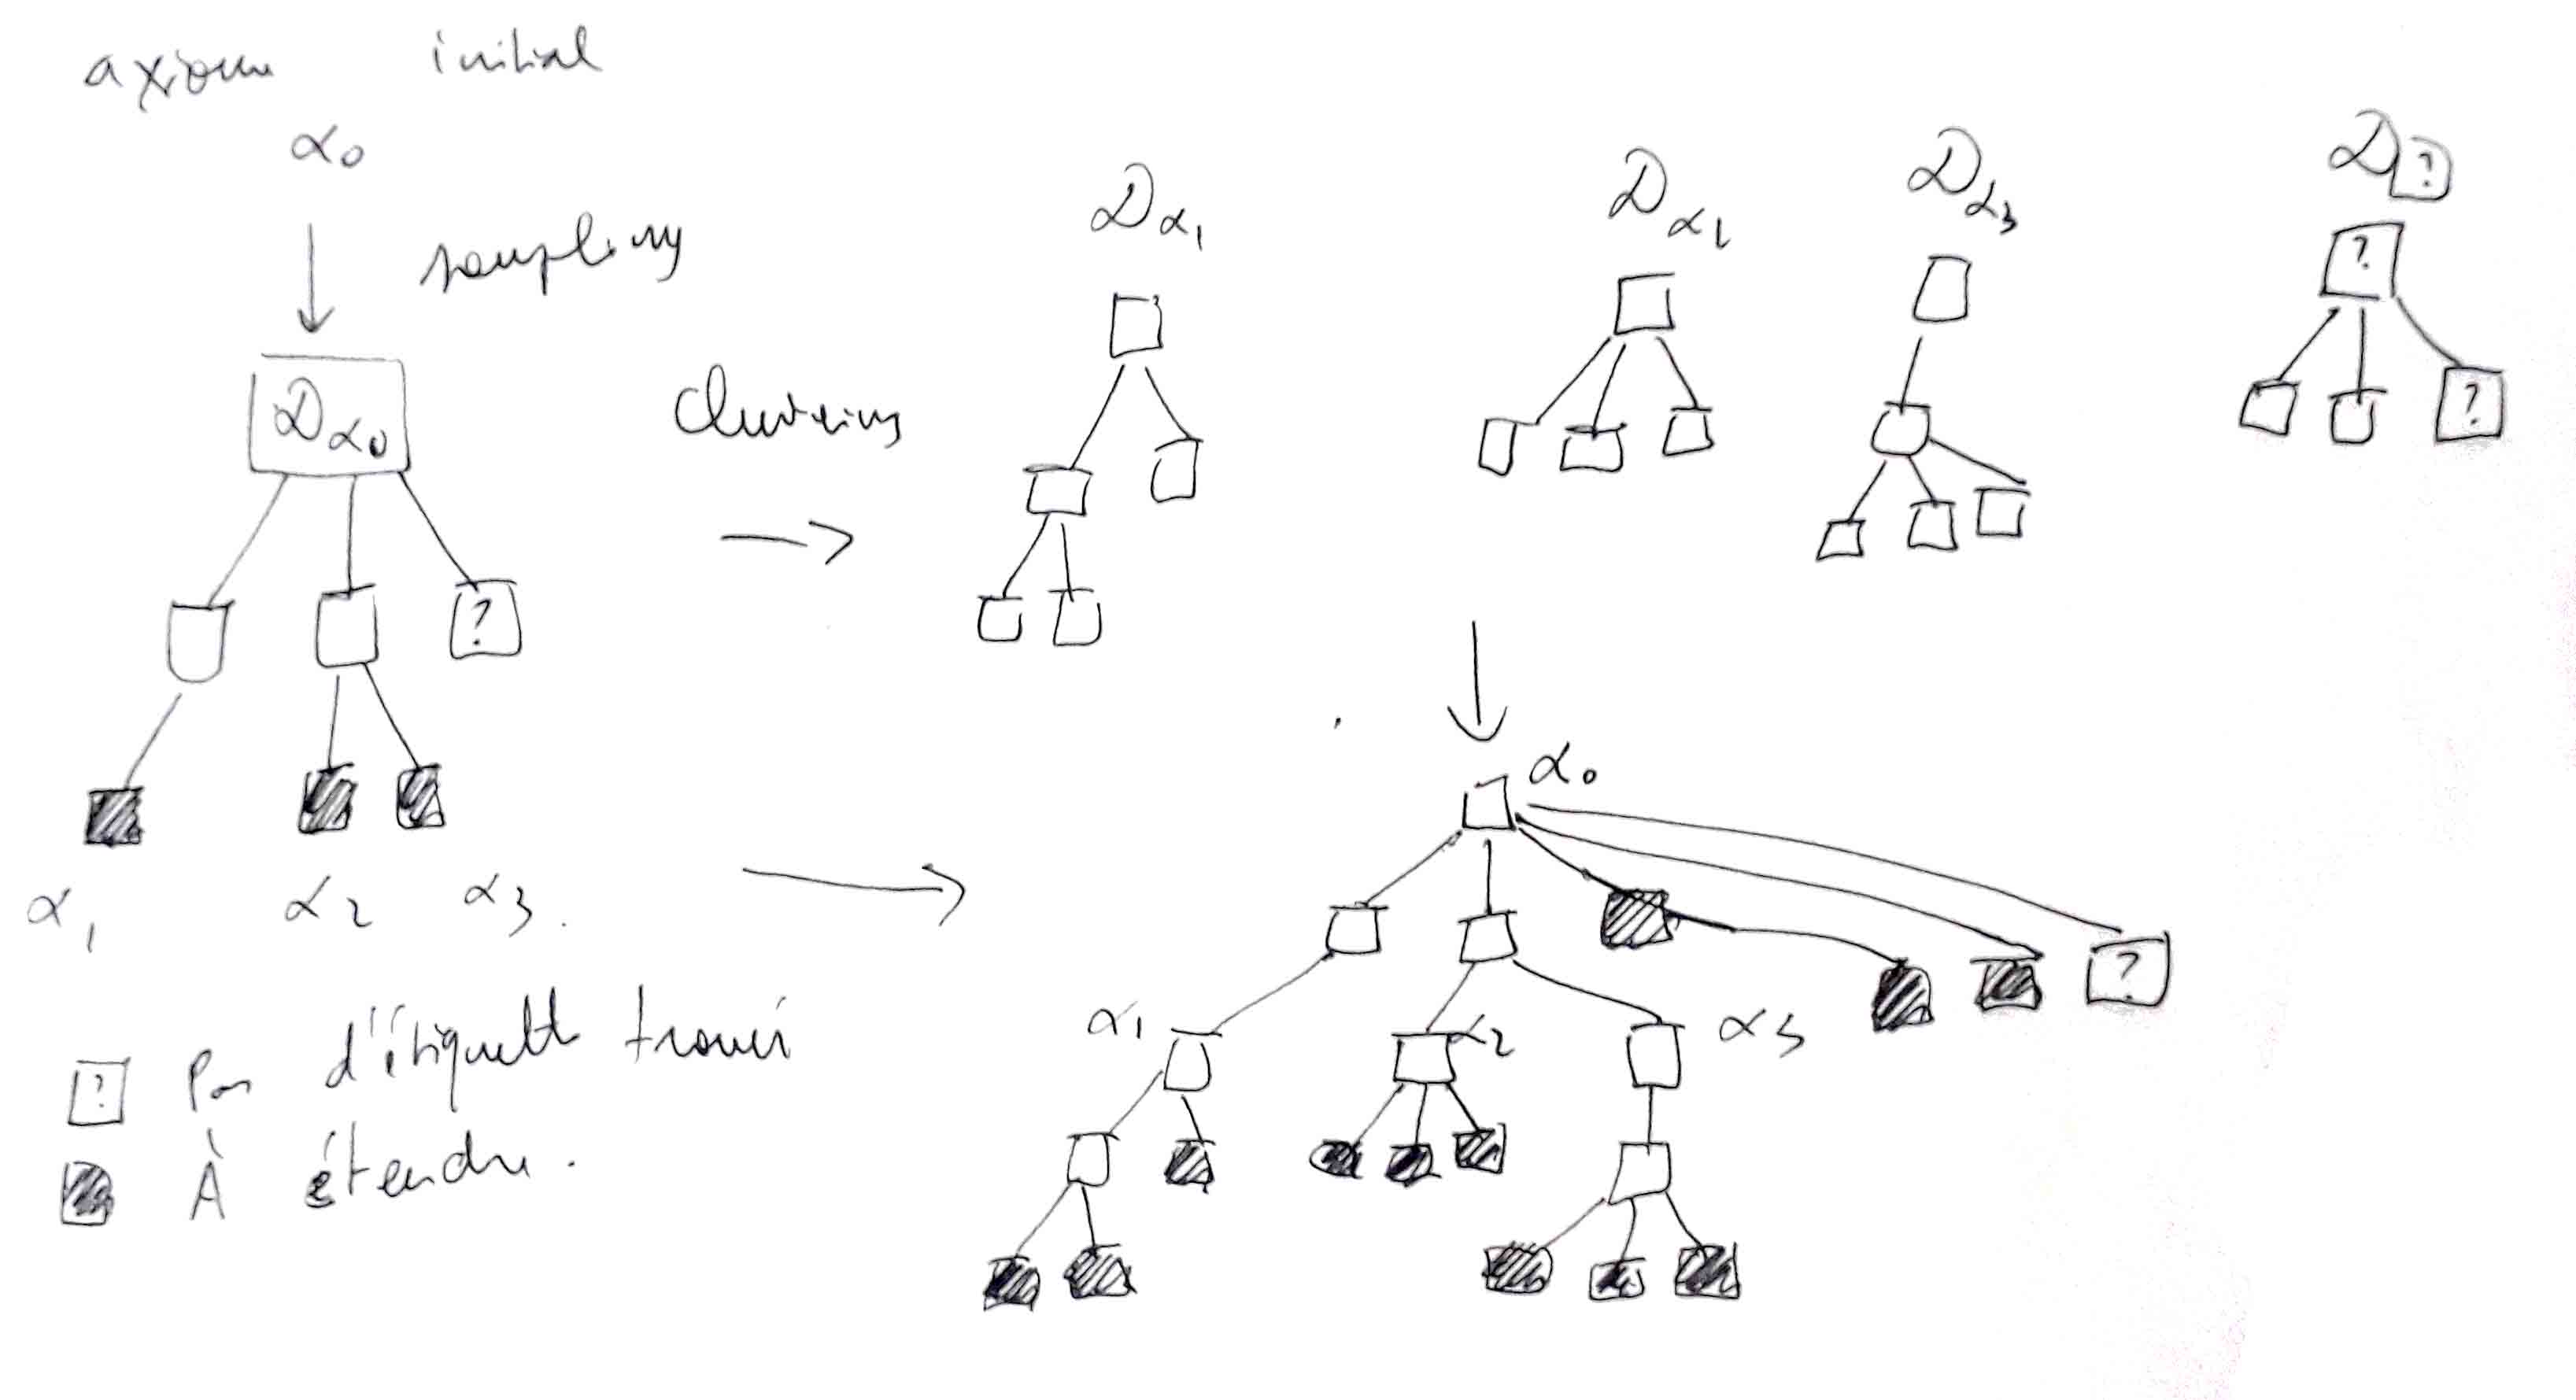
\includegraphics[width=\textwidth]{img/expressive_extraction_overview.jpg}
    \caption{(Provisoire) Principe général pour l'expansion d'arbres. À partir d'un axiome initial $\alpha_0$, un arbre est construit, et trois nouveaux axiomes $\alpha_1, \alpha_2, \alpha_3$. Trois nouveaux arbres sont construits, et ajoutés à l'arbre initial. Le procédé est répété, jusqu'à obtenir une taxonomie expressive complète.}
    \label{fig:my_label}
\end{figure}
\todo{Insérer la vraie figure pour l'expansion d'arbre}

\paragraph{Seuil adaptatif} On expérimente également une variante de l'algorithme précédent, dans laquelle le seuil $\delta$ pour l'extraction d'axiome varie au cours du temps : au début, le seuil de validité des axiomes est fixé à une valeur initiale élevée $\delta = \delta_\text{init}$; puis, à chaque fois que la file d'axiome $A$ est vidée, on diminue $\delta$ d'une quantité $d\delta$, on ré-initialise $A = \{ \top \}$, et on recommence l'algorithme, jusqu'à atteindre un seuil minimal $\delta_\text{min}$ . Des valeurs typiques sont $\delta_\text{init} = 0.9, d\delta = 0.1, \delta_\text{min} = 0.5$.

Partir avec un seuil bas dès le début ne permet pas de discriminer efficacement les axiomes valides des axiomes invalides; au contraire, conserver un seuil élevé tout au long de l'algorithme conduit à écarter des axiomes valides : en effet, les graphes de connaissance étant incomplets et bruités – certaines relations manquent, des triplets peuvent être erronés etc., un axiome valide peut être imparfaitement vérifié. La technique du seuil adaptatif permet de contourner en partie cette limitation, en imposant d'abord un seuil haut qui permet de créer une ossature fiable pour la taxonomie, puis en relâchant ce seuil pour aggréger de nouveaux axiomes plus incertains.



% Rappeler le principe général
% 
% Exposer le principe de récursivité avec un schéma
% 
% Modalités de retirage
% 
% Expérimentation avec/sans retirage
% 
% Seuil adaptatif


\subsection{Extraction d'axiomes}
\label{subsec:texp-exaxiom}

Une fois que l'on dispose de clusters hiérarchisés, il reste à 
Qui peut être vu comme un étiquetage automatique des clusters

Idée générale

Extraction des atomes

Ici, nous proposons un schéma d'axiome extraction très simple, basé sur des statistiques d'occurrence au sein d'un cluster. Toutefois, la méthode peut s'adapter à beaucoup d'autres algorithmes d'extraction d'axiomes. 

\subsubsection{Couverture, spécificité et score de partition}
Soit $C = \{e_1, e_2, \ldots, e_n \} \subseteq \Ent$ un cluster contenant $n$ entités. Si $C$ n'est pas une feuille, alors il a deux sous-clusters gauche et droit, notés $L$ et $R$, et contenant respectivement $n_1$ et $n_2$ entités, avec $n = n_1 + n_2$. En notant $\sqcup$ l'union disjointe, on a donc :
\begin{equation}
C = L \sqcup R
\end{equation}
Pour un axiome logique $A$ et une entité $x \in \Ent$, on note $A(x)$ si $x$ vérifie l'axiome $A$. On se propose d'expliquer la séparation du cluster $C$ en ses deux sous-clusters, c'est-à-dire d'identifier des axiomes qui sont vrais dans l'un des clusters mais pas dans l'autre. Ce choix a d'abord été fait dans le but de mieux comprendre le fonctionnement du regroupement hiérarchique et d'analyser l'arbre de clustering obtenu. Toutefois, il est apparu que cette approche pouvait servir également à étiquetter des clusters, et donc à leur attribuer des axiomes.

Expliquer la division de $C$ en $L \sqcup R$ nécessite de trouver un axiome $A$ tel que $A$ est valide pour tous les éléments de $L$ et pour aucun élément de $R$ :
\begin{equation}
    \left(\forall x \in L, A(x)  \right) \land \left(\forall x \in R, \neg A(x) \right)
\end{equation}
Soit, de manière équivalente :
\begin{equation}
    \forall x \in C = L \sqcup R, A(x) \oplus (x \in R)
    \label{eq:exaxiom-xor-def}
\end{equation}
Avec $\oplus$ l'opérateur «ou exclusif». L'équation \ref{eq:exaxiom-xor-def} signifie qu'une entité de $C$ ne peut pas à la fois être dans $R$ et vérifier $A$, et elle ne peut pas non plus être dans $L$ sans vérifier $A$. Cette équation correspond au cas optimal où il existe un axiome qui divise parfaitement $C$ en $L$ et $R$ : en pratique, la plupart des clusters ne peuvent pas être parfaitement divisés, et il nous faut donc mesurer à quel point on se trouve de l'optimalité. Pour cela, on commence par définir la \textit{précision} d'un axiome $A$ par rapport à un ensemble d'éléments $E \sqsubset \Ent$ quelconque comme la proprtion d'éléments de $E$ qui vérifient $A$ :
\begin{equation}
    \text{prec}(A, E) = \frac{|\{ x \in E, A(x)\}|}{| E |}
\end{equation}
On mesure alors la capacité d'un axiome $A$ à expliquer la division $C = L \sqcup R$ avec deux métriques : d'une part, sa \textit{couverture}, définie comme la proportion d'éléments de $L$ qui vérifient $A$; d'autre part, sa \textit{spécificité}, qui indique la proportion d'éléments de $R$ qui ne vérifient pas $A$. Ces deux métriques se calculent à partir de la précision comme suit :
\begin{align}
    \text{cov}_{L \sqcup R}(A) &= \text{prec}(A, L) \\
    \text{sep}_{L \sqcup R}(A) &= 1 - \text{prec}(A, R)
\end{align}
On combine ces deux mesures en un seul indicateur synthétique, que l'on appelle le \textit{score de partition} de $A$, à l'aide d'une moyenne harmonique :
\begin{equation}
    \text{part}_{L \sqcup R}(A) = \left(  \text{cov}_{L \sqcup R}(A)^{-1} + \text{sep}_{L \sqcup R}(A)^{-1} \right)^{-1}
\end{equation}

On peut vérifier que l'on retrouve bien l'intuition derrière l'équation \ref{eq:exaxiom-xor-def}. La proportion d'éléments qui vérifient la condition de séparation \ref{eq:exaxiom-xor-def} est donnée par :
\begin{equation}
    \text{xor}(A) = \frac{| \{x \in C : A(x) \oplus (x \in R) \}|}{| C |}
\end{equation}
Par définition de l'opérateur ou exclusif, on peut écrire :
\begin{equation}
    n \cdot \text{xor}(A) = |\{x \in C: (A(x) \land \neg (x \in R) \lor (x \in R \land \neg A(x)) \}|
\end{equation}
Puis, comme $C$ est l'union disjointe $L$ et $R$, si $x \in C$, alors $\neg (x \in R) = x \in L$ et on a donc :
\begin{align*}
    n \cdot \text{xor}(A) &= |\{x \in L: (A(x)\} \sqcup \{x \in R : \neg A(x)) \}| \\
    &= |\{x \in L: (A(x)\} | + | \{x \in R : \neg A(x)) \}|  \\
    &= |\{x \in L: (A(x)\} | + | \{x \in R \} \setminus \{x \in R : A(x)) \}| \\
    &= n_1 \cdot \text{prec}(A, L) + n_2 - n_2 \cdot \text{prec}(A, R) \\
    &= n_1 \cdot \text{cov}(A) + n_2 \cdot \text{spe}(A) \\
\end{align*}
Soit finalement :
\begin{equation}
    \text{xor}(A) = \frac{n_1 \cdot \text{cov}(A) + n_2 \cdot \text{spe}(A)}{n_1 + n_2}
\end{equation}

Notation\todo{Déplacer ceci} : pour un axiome $A$ et un ensemble d'entités $E \sqsubset \Ent$, on note $A(E)$ l'ensemble des éléments de $E$ qui vérifient $A$ :
$$
A(E) = \{ x \in E : A(x) \}
$$
On vérifie facilement que les propriétés suivantes sont vraies :
\begin{align}
    & \top(E) = E  \\
    & \bot(E) = \varnothing  \\
    & (A \land B)(E) \subseteq A(E) \label{eq:prop-ax-and} \\
    & A(E) \subseteq (A \lor B)(E)  \\
    & E \subset E' \implies A(E) \sqsubset A(E') 
\end{align}
Et on a :
\begin{align}
    \pre_{L \sqcup R}(A) &= \frac{|A(L) |}{|L|} \\
    \rec_{L \sqcup R}(A) &= 1 - \pre(A, R) \\
\end{align}

Avant de présenter l'extraction d'axiome proprement dite, relevons quelques propriétés de ces métriques. Soit $A, B$ deux axiomes. Alors :
\begin{align}
\cov(A \land B, E) &= \frac{|(A \land B)(L) |}{| L |} \\
                &\leq \frac{|A(L) |}{| L |} \text{ d'après l'équation \ref{eq:prop-ax-and}} \\
                &\leq \cov(A) \label{eq:prop-cov-land}
\end{align}
Il suit que :
\begin{align}
\cov(A \lor B) &= \frac{|\{ x \in L : A(x) \lor B(x) \}|}{| L |} \\
  &= \frac{|\{ x \in L : A(x) \}| + |\{ x \in L :  B(x) \} - |\{ x \in L : A(x) \land B(x) \}||}{|E|} \\
  &= \cov(A) + \cov(B) - \cov(A \land B)
\end{align}
Or, d'après la relation \ref{eq:prop-cov-land}, $\cov(B) \geq \cov(A \land B)$, d'où finalement :
\begin{equation}
    \cov(A \lor B) \geq \cov(A)
\end{equation}
Or, comme $\spe(x) = 1 - \cov(x)$, on peut obtenir les relations suivantes :
\begin{align}
    \spe(A \land B) &\geq \spe(A) \label{eq:prop-spe-land} \\
    \spe(A \lor B) &\leq \spe(A) 
\end{align}

\subsubsection{Construction d'axiomes complexes par améliorations successives d'axiomes atomiques}

On dispose d'un moyen pour évaluer la capacité d'un axiome $A$ à expliquer la partition d'un cluster en deux sous-clusters. Il reste à définir une procédure pour construire de tels axiomes. Pour cela, on définit d'abord des types d'axiomes primitifs, appelés des \textit{axiomes atomiques} ou simplement \textit{atomes} dans la suite; on extrait, pour chaque cluster, une liste d'axiomes atomiques, puis on combine ces atomes au moyen de conjonctions et de disjonctions pour produire des axiomes plus complexes.

On considère les types d'axiomes atomiques suivants :
\begin{itemize}
    \item les classes $C$, aussi appelés concepts en logique descriptive, comme par exemple \dbo{Agent}, \dbo{Person} ou \dbo{Place};
    \item les restrictions de la forme $\exists R.C$ avec $C$ une classe, par exemple $\exists \dbo{locatedIn}.\dbo{Country}$, qui contient toutes les entités situées dans un pays ;
    \item les restrictions de la forme $\exists R.\{v\}$ avec $v \in \Ent$ une entité, tel que $\exists \dbo{locatedIn}.\{\dbr{Canada}\}$ pour représenter l'ensembles des entités situées au Canada;
    \item les restrictions de la forme $\exists R.t$, avec $t$ représentant les littéraux d'un type $t$ donné, comme par exemple $\exists \dbo{birthDate}.\texttt{xsd:date}$ l'ensemble des entités dont la date de naissance est du type \texttt{xsd:date};
\end{itemize}

Pour chaque entité $x$ du cluster d'entrée, on extrait l'ensemble des triplets $(x, r, y)$ dont $x$ est le sujet. Si $r$ est la relation \rdf{type}, alors $y$ représente une classe, et le triplet $(x, r, y)$ est transformé en l'axiome atomique $y$. Si $y$ est un littéral, on extrait son type $t$, et on obtient l'axiome atomique $\exists r.t$. Autrement, on liste les classes $C_1, C_2, \ldots, C_m$ dont $y$ fait partie, et on extrait les axiomes atomiques $\exists r.\{y\}, \exists r.C_1, \ldots, \exists r.C_m$. On obtient ainsi une liste d'axiomes atomiques $\mathcal{A}_\text{atomes}$ pour l'entièreté du cluster; cette liste est filtrée et seuls les atomes vérifiés par plus de $\delta_\text{filtre} = 10\%$ des entités du cluster sont conservés.

Ensuite, on génère une liste d'axiomes candidates $\cal{A}_\text{candidats}$ à partir de cette liste d'axiomes atomiques. Initialement, les axiomes candidats sont simplement les axiomes atomiques. On évalue chaque axiome $a$ parmi les candidats, en calculant sa couverture, sa spécificité et son score. On compare alors ce score à un seuil $\delta$, par exemple $\delta = 0.9$. Si $\text{cov}(a) < \delta$, l'axiome $A$ ne couvre pas assez d'entités : on l'améliore alors itérativement en ajoutant des clauses OU. Pour chaque axiome atomique $b$, on génère un nouvel axiome candidat $a \lor b$, et on l'ajoute à la liste des axiomes candidats. D'après l'équation \ref{eq:prop-cov-land}, $\cov(a \lor b) \geq \cov(a)$.
À l'inverse, si $\spe(a) < \delta$, alors l'axiome est insuffisamment spécifique : il est vérifié par trop d'éléments de $R$. Suivant l'équation \ref{eq:prop-cov-land} : $\forall b, \spe(a \land b) \geq \spe(a)$, on peut améliorer cette spécificité en ajoutant une conjonction. Pour tout axiome atomique $b$, on génère l'axiome $a \land b$ et on l'ajoute à la liste des axiomes candidats. 
Si on a à la fois $\spe(a) < \delta$ et $\cov(a) < \delta$, alors l'axiome $a$ ne permet pas d'expliquer la partition $C = L \sqcup R$ et il est retiré de la liste des candidats. Enfin, si $\cov(a) > \delta$ et $\spe(a) > \delta$, l'axiome est conservé tel quel.

À chaque itération, on limite le nombre de candidats qui sont améliorés (c'est-à-dire étendus par des disjonctions ou des conjonctions) : seuls les $N_\text{ax}$ axiomes candidats avec le plus haut score de partition sont conservés, avec $N_\text{ax}$ un paramètre fixé empiriquement, typiquement $N_\text{ax} = 10$. La recherche d'axiomes s'arrête lorsqu'il n'y a plus d'axiomes candidats à améliorer ou lorsque le nombre d'itérations dépasse une certaine limite $N_\text{iter}$.

Le résultat de cet algorithme est un ensemble $\cal{A}(L)$ (éventuellement vide) d'axiomes capables de qualifier le sous-cluster $L$ par opposition au sous-cluster $R$, avec les scores associés. Si $\cal{A}(L) = \varnothing$, aucun axiome satisfaisant aux critères n'a été trouvé, et le cluster $L$ n'est donc pas étiquetté. Sinon, on étiquette $L$ avec l'axiome de plus haut score :
\begin{equation}
    \alpha^*(L) = \argmax_{a \in \cal{A}(L)}(\xscore(a))
\end{equation}

\todo{Mentionner l'autre idée (TF-IDF) ?} %Autre principe : TF-IDF based

\subsubsection{Détails pratiques}

Axiomes vus comme des vecteurs booléens. Le tout est vu comme une matrice booléenne, opérations rapides sur les lignes et les columns

Expliquer la traduction matricielle de $\cov, \spe, \xscore \ldots$

\iffalse

\subsection{Algorithme général}
% Raffinements
\subsubsection{Vue d'ensemble}

Extraction de taxonomie à partir des axiomes

Choix des seuils

Discussion sur les paramètres

\subsubsection{Diminution du seuil}
 % Déplacer en section 5.2.1 ?
% À faire : mentionner quelque part 


\subsubsection{Phase finale}

Phase finale : ajout des classes manquantes (si disponible), restriction des patterns
\fi 

\section{Évaluation et discussion}

\subsection{Évaluation quantitative par comparaison avec l'ontologie existante}
\subsection{Évaluation qualitative des axiomes obtenus}

%
%
% ??????????????
%
%
%             % Troisième thème (Doctorat) ou effacez ce fichier si vous êtes à la Maîtrise.
\Chapter{CONCLUSION}\label{sec:Conclusion}


% On résume ici le contenu du mémoire
% relevons ses limites et proposons des pistes pour les surmonter


%%
%%  SYNTHESE DES TRAVAUX / SUMMARY OF WORKS
%%
\section{Synthèse des travaux}


Dans ce travail, on s'est intéressé au problème de l'extraction de taxonomie à partir d'un graphe de connaissance. Plus particulièrement, notre idée était d'utiliser les plongements vectoriels pour identifier des groupes d'entités cohérents, et établir des liens taxonomiques entre ces groupes. L'objectif est donc d'établir une hiérarchie entre les classes existantes, mais aussi de pouvoir découvrir et caractériser de nouvelles classes. 

Pour cela, nous commençons par une étude des modèles de plongement vectoriel, sous l'angle de la \textit{séparabilité} : nous mesurons la capacité des modèles de plongement à plonger des entités de types différents dans des régions différentes de l'espace. % Sur cette tâche, la hiérarchie entre les modèles n'est pas celle que l'on obtient sur les tâches d'évaluation usuelles.
%
Cette nouvelle tâche permet de nuancer l'état de l'art en matière de plongements vectoriels : en effet, sur les tâches d'évaluation usuelles que sont la prédiction de lien ou la complétion de triplets, TransE obtient des performances inférieures à des modèles plus expressifs comme ComplEx; ici, la hiérarchie est inversée.


Nous abordons ensuite le problème de l'extraction de taxonomie à partir d'un graphe de connaissance, en se basant sur DBpedia. Puisque l'on veut pouvoir identifier de nouvelles classes, on se base sur un regroupement non-supervisé des plongements vectoriels : cela nous permet d'extraire une structure d'arbre sur les groupes d'entités sans aucune supervision. À partir de cette structure, on peut décliner l'approche pour obtenir une taxonomie expressive ou non-expressive.

%si l'on injecte une liste de types connus
Si l'on fait correspondre ces groupes à des types connus, on obtient une taxonomie non-expressive. Au chapitre \ref{chap:te}, nous proposons deux méthodes pour établir cette correspondance, l'une qui détermine une injection optimale des types vers les groupes, l'autre qui propose une association multiple entre les uns et les autres. Nous montrons que ces deux méthodes sont capables d'égaler et même de dépasser une méthode basée sur un regroupement supervisé.

Au chapitre \ref{chap:texp}, on associe au contraire les groupes à des axiomes logiques expressifs, et on ajoute un mécanisme d'itération pour fiabiliser le résultat : d'une part, le regroupement hiérarchique est répété sur des groupes d'entités de plus en plus spécifiques, et d'autre part la taxonomie extraite est étendue petit à petit sur la base de ce regroupement. Nous obtenons ainsi une taxonomie expressive de DBpedia.


% Au-delà de l'extraction de taxonomie proprement dite, ce travail nous permet d'évaluer les modèles de plongement; la hiérarchie obtenue entre les modèles re

%met en perspective les résultats

%d'une part, la hiérarchie que nous obtenons entre modèles n'est pas celle obtenue sur les tâches d'évaluation usuelles; d'autre part, 

\iffalse {
Nous montrons au chapitre \ref{chap:te} que cette méthode est capable d'égaler, et même de dépasser une méthode basée sur un regroupement supervisé. 

on extrait une taxonomie non-expressive

Dans le chapitre \ref{chap:te}, on montre qu'il est possible, avec un regroupement non-supervisé, d'égaler et même de dépasser une méthode basée sur un regroupement supervisé. Pour cela, nous proposons deux approches pour associer des groupes d'entités à des types existants, l'une qui trouve une injection optimale des types vers les groupes, l'autre qui propose une association multiple entre les uns et les autres. Les résultats obtenus fournissent également une évaluation des modèles de plongement, et montrent qu'un modèle simple est capable de surpasser des modèles plus complexes sur la tâche d'extraction de taxonomie.

% Cette tâche nous fournit également un nouveau moyen d'évaluer les modèles de plongement

Nous proposons ensuite une méthode pour extraire une taxonomie non-expressive d'un graphe de connaissance. 


La plupart des méthodes utilisant des plongements sont incapables d'identifier de nouvelles classes


pareil chap par chap 
séparabilité : la hiérarchie n'est pas la même que sur le link prediction + comportemnt différencié selon les modèles

Au chapitre \ref{chap:kge}, nous avons mesuré la capacité de plusieurs modèles de plongement à plonger des entités de types différents dans des régions différentes de l'espace. Sur cette nouvelle tâche, la hiérarchie entre modèles n'est pas celle que l'on obtient sur la complétion ou la classification de triplets, ce qui indique 



Au chapitre \ref{chap:te}, nous proposons une méthode d'extraction automatique de taxonomie, qui se distingue des méthodes existantes par le regroupement hiérarchique non-supervisé d'entités, à partir de leurs plongements vectoriels. Ce regroupement hiérarchique est couplée à une étape d'association entre groupes d'entités et types, pour laquelle nous proposons deux solutions : l'une est basée sur une injection des types vers les groupes; l'autre sur une association multiple entre types et groupes. Quoique ces deux méthodes obtiennent des résultats proches dans nos expériences, 

Nous étendons cette idée à l'extraction de taxonomie expressive, 
}
\fi 
\section{Limitations et pistes d'améliorations}

Nous identifions ici quelques limitations des travaux présentés ici, et proposons des pistes pour les surmonter. Nous esquissons aussi des directions de recherche pour poursuivre ou prolonger le travail entamé dans ce mémoire.


\paragraph{Modèles de plongement}

Dans tous les travaux présentés ici, on s'est restreint à évaluer six modèles de plongement, entraînés avec les hyperparamètres par défaut. Augmenter le nombre de modèles entraînés et faire varier ces hyperparamètres constitue donc une première piste pour affiner et systématiser les résultats obtenus, à la fois pour la séparabilité et l'extraction de taxonomie. 

Sur la question des hyperparamètres, \cite{kadlec2017knowledge} a montré que la recherche d'hyperparamètres était une étape cruciale pour la tâche de prédiction de lien; si cette conclusion s'applique également à l'extraction de taxonomie, alors une recherche rigoureuse d'hyperparamètres s'impose : non seulement pour obtenir les meilleurs résultats possibles, mais aussi pour comprendre l'interaction entre les choix de modélisation effectués par un modèle de plongement donné, les valeurs des différents hyperparamètres et les données d'entrée. 
% Cela permettrait de mieux comprendre . 
% pour expliquer quelle part de la variabilité des résultats d'un modèle à l'autre s'explique par les choix d'hyperparamètres ou les propriétés intrinsèques des modèles.

Quant aux modèles de plongement, de nombreuses approches ont été proposées qui obtiennent de bons résultats sur les jeux d'évaluation usuelles. Dans la lignée des modèles présentés ici, on peut citer des modèles algébriques comme HolE \cite{hole2016} et SimplE \cite{simple2018}, des modèles géométriques, comme PTransE \cite{ptranse} qui étend TransE à des chemins dans le graphe, plutôt qu'à des triplets isolés, ou RotatE \cite{rotate2019}, qui choisit de représenter les relations par des rotations dans l'espace. D'autres approches incluent des modèles neuronaux, comme R-GCN \cite{rgcn2018}, ProjE \cite{proje2017} ou ConvE \cite{conve2018}, ou l'utilisation de géométries non-euclidiennes \cite{nickel2017poincare, nickel2018learning}.

Pour l'évaluation des modèles, qui fait l'objet du chapitre \ref{chap:kge}, notre tâche de séparabilité se révèle incomplète : idéalement, on souhaiterait trouver un mode d'évaluation qui reflète les performances des modèles sur l'extraction taxonomique. Or, RDF2Vec obtient de meilleurs résultats que TransE pour la séparabilité, alors que TransE est supérieur à RDF2Vec sur la tâche d'extraction.  
Pour remédier à ce problème, on pourrait adjoindre une tâche de \textit{regroupement} à la tâche de séparabilité, pour vérifier le comportement des modèles de plongement vis-à-vis des algorithmes de regroupement. 
On peut par exemple tirer des entités appartenant à $k$ classes différentes, puis appliquer un algorithme des $k$-moyennes sur les plongements de ces entités, et finalement mesurer si le partitionnement obtenu recoupe bien les $k$ classes initiales.

\paragraph{Extraction de taxonomie non-expressive}

Notre approche pour l'extraction automatique de taxonomie non-expressive est limitée par l'étape de regroupement. Pour des questions de performance, la taille des données à regrouper est limitée, ce qui, d'une part, empêche d'utiliser l'intégralité des entités du graphe, et d'autre part, entraîne la décroissance exponentielle du nombre d'entités par classes. Ces deux facteurs compliquent le traitement des classes rares ou très spécifiques. En l'état, notre méthode n'est donc pas applicable à toute la taxonomie DBpedia.

Une solution possible consisterait à itérer la méthode Soft Mapping avec des données d'entrée tirées aléatoirement dans le graphe : à chaque étape, on tire des entités aléatoirement, on les regroupe, et on calcule la probabilité des axiomes de subsumption. On peut alors maintenir une matrice contenant ces probabilités, et la mettre à jour à chaque étape. De plus, on peut utiliser la géométrie des plongements pour tirer les entités dans une région donnée de l'espace, ce qui permettrait d'augmenter la spécificité des données et donc de la taxonomie extraite – il s'agirait en fait d'adapter la méthode expressive présentée à la section \ref{subsec:texp-clustering} au cas où l'on n'a pas accès au graphe complet.


\paragraph{Extraction de taxonomie expressive}


Notre méthode d'extraction d'axiomes présente plusieurs limites : d'une part, les axiomes atomiques sont limités et laissent de côté les relations inverses, la composition de relations, les restrictions universelles, etc. D'autre part, on combine à chaque étape un axiome (complexe ou non) avec un atome : on ne peut donc pas combiner un axiome complexe avec un autre axiome complexe, ce qui interdit par exemple des axiomes de la forme $(A \land B) \lor (C \land D)$. Il serait également intéressant d'expérimenter d'autres approches pour l'extraction d'axiomes : comme l'espace de recherche est un sous-ensemble d'entités de petite taille et sémantiquement cohérent, il devrait être possible d'employer des méthodes plus complexes et capables d'extraire des axiomes plus expressifs.

Quant aux faiblesses des taxonomies expressives extraites par notre approche, elles ont été discutées à la section \ref{subsec:texp-reslts-limits} : les axiomes extraits sont inégalement informatifs, parfois redondants ou trop spécifiques. La piste d'amélioration la plus évidente consiste à expérimenter des valeurs différentes pour les paramètres. Ceux-ci sont en effet nombreux, à chaque étape : on peut modifier les modalités du tirage aléatoire, la méthode de regroupement, l'ordre de parcours de l'arbre de clustering et sa profondeur maximale, le mode d'extracion (mono-niveau ou multi-niveaux), le nombre d'étapes et l'évolution du seuil $\delta$. Toutefois, pour systématiser une telle recherche, il est nécessaire de concevoir une méthode d'évaluation qualitative fiable des taxonomies produites. Pour ce faire, on peut envisager la démarche suivante : identifier des tâches externes susceptibles de tirer profit d'axiomes logiques (par exemple, typage automatique d'entités, réponse automatique à des questions, ou autre), et comparer, sur ces tâches, les performances d'un modèle utilisant seulement le graphe aux performances d'un modèle utilisant à la fois le graphe et la taxonomie prédite. On obtient ainsi une évaluation indirecte de cette taxonomie, qui permet de mesurer son utilité pratique.

% ce qui devrait autoriser l'emploi de méthodes 


Enfin, puisque l'on dispose de plongements vectoriels pour les entités, et d'axiomes logiques pour qualifier ces groupes, une direction de recherche intéressante serait de chercher une représentation vectorielle des axiomes logiques, afin d'obtenir une représentation unifiée pour les entités, les relations, les classes et les axiomes. 
Cela suppose de traduire géométriquement des opérateurs logiques tels que la négation, la conjonction ou la disjonction; ce problème est discuté par
\cite{gutierrez2018knowledge}, et une solution est esquissée par \cite{hao2019universal}.
         % Conclusion.
%\backmatter
\ifthenelse{\equal{\Langue}{english}}{
	\renewcommand\bibname{REFERENCES}
	\bibliographystyle{IEEEtran.bst}
	\bibliography{Document}			% Bibliography style. 
}{
	\renewcommand\bibname{RÉFÉRENCES}
	\bibliographystyle{IEEEtran-francais.bst}    % Style de la bibliographie. 
	\bibliography{Document}
}
%
\ifthenelse{\equal{\AnnexesPresentes}{O}}{
	\appendix%
	\newcommand{\Annexe}[1]{\annexe{#1}\setcounter{figure}{0}\setcounter{table}{0}\setcounter{footnote}{0}}%
	%%
%%  Annexes
%%
%%  Note: Ne pas modifier la ligne ci-dessous. / Do not modify the following line.
\ifthenelse{\equal{\Langue}{english}}{
	\addcontentsline{toc}{compteur}{APPENDICES}
}{
	\addcontentsline{toc}{compteur}{ANNEXES}
}



\Annexe{ARTICLE}

On inclut à la page suivante l'article \href{https://dl.acm.org/doi/10.1145/3391274.3393637}{\textit{What is the Schema of your Knowledge Graph: Leveraging Knowledge Graph Embeddings and Clustering for Expressive Taxonomy Learning}}, co-écrit avec Amal Zouaq et présenté à la conférence SBD 2020. Son contenu correspond aux chapitres \ref{chap:kge} et \ref{chap:texp} du présent mémoire.
% \textit{International Workshop  on Semantic Big Data} 2020

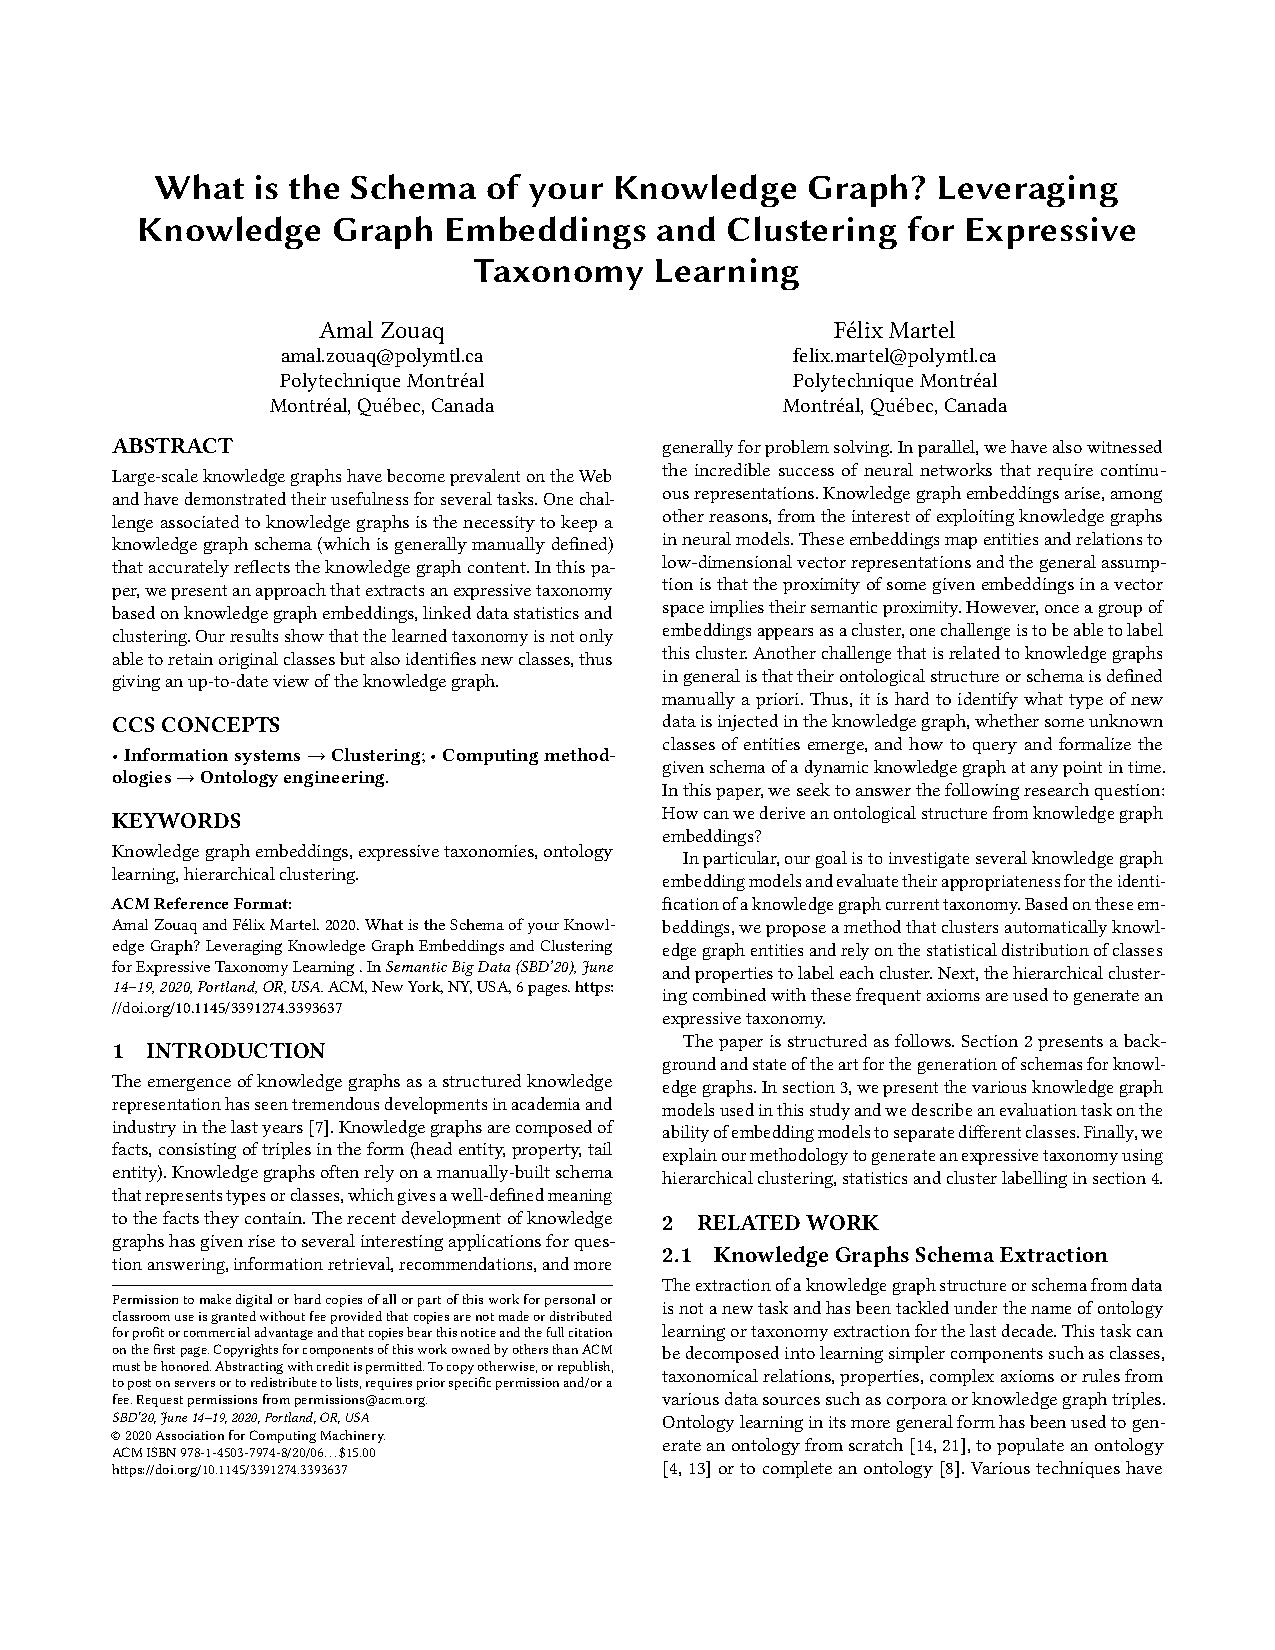
\includepdf[pages=-]{sigmod-article.pdf}


\Annexe{RÉSULTATS COMPLETS POUR L'EXTRACTION DE TAXONOMIE}
\label{ann:results}
Le tableau \ref{tab:te-full-results} présente les résultats complets de l'extraction de taxonomie, et inclut notamment les modèles, les métriques et les critères de liaison qui ont été omis à la section \ref{subsec:te-results}. Dans ce tableau, «cos», «euc», «l1» désignent respectivement les distances cosinus, euclidienne et $L_1$, tandis que «max», «min», «moy» et «ward» désignent le saut maximum, le saut minimum, le saut moyen et le critère de Ward.
%\begin{table}[htbp]
%\centering
%\caption{Caption}
%\label{tab:my_label}
\begin{longtable}{|llll|ccc|ccc|}
    \caption{Résultats complets pour l'extraction de taxonomie présentée à la section \ref{subsec:te-results}.}
    \label{tab:te-full-results}
    \hline 
	&		&		&		&	\multicolumn{3}{c|}{Directe} & \multicolumn{3}{c|}{Transitive}   \\
Plongements	&	Méthode	&	Métrique	&	Liaison	&	$p$	&	$r$	&	$F_1$	&	$p$	&	$r$	&	$F_1$	\\
\hline \endhead
\hline \endfoot
ComplEx	&	MLI	&	cos	&	max	&	0.47	&	0.38	&	0.42	&	0.77	&	0.5	&	0.61 \\ 
ComplEx	&	MLI	&	euc	&	max	&	0.4	&	0.36	&	0.38	&	0.73	&	0.53	&	0.62 \\ 
ComplEx	&	MLI	&	l1	&	max	&	0.38	&	0.33	&	0.35	&	0.68	&	0.57	&	0.62 \\ 
DistMult	&	MLI	&	cos	&	max	&	0.49	&	0.41	&	0.44	&	0.65	&	0.53	&	0.59 \\ 
DistMult	&	MLI	&	euc	&	max	&	0.29	&	0.23	&	0.26	&	0.52	&	0.42	&	0.46 \\ 
DistMult	&	MLI	&	l1	&	max	&	0.26	&	0.19	&	0.22	&	0.49	&	0.36	&	0.42 \\ 
RDF2Vec	&	MLI	&	cos	&	max	&	0.3	&	0.23	&	0.26	&	0.58	&	0.35	&	0.44 \\ 
RDF2Vec	&	MLI	&	euc	&	max	&	0.5	&	0.3	&	0.37	&	0.79	&	0.35	&	0.49 \\ 
RDF2Vec	&	MLI	&	l1	&	max	&	0.29	&	0.31	&	0.3	&	0.48	&	0.54	&	0.51 \\ 
TransD	&	MLI	&	cos	&	max	&	0.05	&	0.05	&	0.05	&	0.19	&	0.21	&	0.2 \\ 
TransD	&	MLI	&	euc	&	max	&	0	&	0	&	0	&	0.11	&	0.22	&	0.15 \\ 
TransD	&	MLI	&	l1	&	max	&	0.06	&	0.06	&	0.06	&	0.18	&	0.3	&	0.23 \\ 
TransE	&	MLI	&	cos	&	max	&	0.76	&	0.64	&	0.69	&	0.92	&	0.64	&	0.75 \\ 
TransE	&	MLI	&	euc	&	max	&	0.55	&	0.48	&	0.52	&	0.86	&	0.53	&	0.66 \\ 
TransE	&	MLI	&	l1	&	max	&	0.72	&	0.64	&	0.68	&	0.94	&	0.58	&	0.72 \\ 
ComplEx	&	MLM	&	cos	&	max	&	0.51	&	0.39	&	0.44	&	0.86	&	0.57	&	0.69 \\ 
ComplEx	&	MLM	&	euc	&	max	&	0.42	&	0.34	&	0.38	&	0.81	&	0.57	&	0.67 \\ 
ComplEx	&	MLM	&	l1	&	max	&	0.42	&	0.31	&	0.36	&	0.84	&	0.55	&	0.67 \\ 
DistMult	&	MLM	&	cos	&	max	&	0.46	&	0.39	&	0.42	&	0.9	&	0.61	&	0.73 \\ 
DistMult	&	MLM	&	euc	&	max	&	0.45	&	0.36	&	0.4	&	0.84	&	0.55	&	0.67 \\ 
DistMult	&	MLM	&	l1	&	max	&	0.33	&	0.17	&	0.23	&	0.7	&	0.31	&	0.43 \\ 
RDF2Vec	&	MLM	&	euc	&	max	&	0.61	&	0.36	&	0.45	&	0.84	&	0.39	&	0.53 \\ 
RDF2Vec	&	MLM	&	cos	&	max	&	0.42	&	0.34	&	0.38	&	0.64	&	0.45	&	0.53 \\ 
RDF2Vec	&	MLM	&	l1	&	max	&	0.39	&	0.38	&	0.38	&	0.52	&	0.53	&	0.53 \\ 
TransD	&	MLM	&	cos	&	max	&	0.03	&	0.03	&	0.03	&	0.24	&	0.15	&	0.19 \\ 
TransD	&	MLM	&	euc	&	max	&	0	&	0	&	0	&	0.12	&	0.15	&	0.13 \\ 
TransD	&	MLM	&	l1	&	max	&	0	&	0	&	0	&	0.12	&	0.15	&	0.14 \\ 
TransE	&	MLM	&	cos	&	max	&	0.7	&	0.59	&	0.64	&	0.88	&	0.65	&	0.75 \\ 
TransE	&	MLM	&	euc	&	max	&	0.49	&	0.41	&	0.44	&	0.89	&	0.55	&	0.68 \\ 
TransE	&	MLM	&	l1	&	max	&	0.71	&	0.66	&	0.68	&	0.95	&	0.68	&	0.79 \\ 
TransH	&	MLM	&	cos	&	max	&	0.08	&	0.02	&	0.03	&	0.77	&	0.1	&	0.17 \\ 
TransH	&	MLM	&	euc	&	max	&	0.17	&	0.02	&	0.03	&	1	&	0.06	&	0.11 \\ 
TransH	&	MLM	&	l1	&	max	&	0.25	&	0.06	&	0.1	&	0.79	&	0.14	&	0.24 \\ 
TransE	&	MLM	&	cos	&	max	&	0.54	&	0.69	&	0.6	&	0.88	&	0.69	&	0.77 \\ 
TransE	&	MLM	&	euc	&	max	&	0.43	&	0.48	&	0.46	&	0.86	&	0.59	&	0.7 \\ 
TransE	&	MLM	&	l1	&	max	&	0.57	&	0.67	&	0.62	&	0.95	&	0.68	&	0.79 \\ 
DistMult	&	MLI	&	euc	&	min	&	0.26	&	0.2	&	0.23	&	0.34	&	0.59	&	0.44 \\ 
TransE	&	MLM	&	cos	&	min	&	-	&	-	&	-	&	-	&	-	&	- \\ 
TransE	&	MLM	&	l1	&	min	&	-	&	-	&	-	&	-	&	-	&	- \\ 
ComplEx	&	MLI	&	cos	&	moy	&	0.53	&	0.5	&	0.52	&	0.78	&	0.7	&	0.74 \\ 
ComplEx	&	MLI	&	euc	&	moy	&	0.54	&	0.45	&	0.49	&	0.71	&	0.63	&	0.67 \\ 
ComplEx	&	MLI	&	l1	&	moy	&	0.54	&	0.47	&	0.5	&	0.76	&	0.65	&	0.7 \\ 
DistMult	&	MLI	&	cos	&	moy	&	0.55	&	0.47	&	0.5	&	0.73	&	0.57	&	0.64 \\ 
DistMult	&	MLI	&	euc	&	moy	&	0.42	&	0.36	&	0.39	&	0.64	&	0.55	&	0.59 \\ 
DistMult	&	MLI	&	l1	&	moy	&	0.33	&	0.3	&	0.31	&	0.58	&	0.54	&	0.56 \\ 
RDF2Vec	&	MLI	&	cos	&	moy	&	0.6	&	0.44	&	0.5	&	0.88	&	0.5	&	0.63 \\ 
RDF2Vec	&	MLI	&	euc	&	moy	&	0.3	&	0.33	&	0.31	&	0.45	&	0.47	&	0.46 \\ 
RDF2Vec	&	MLI	&	l1	&	moy	&	0.4	&	0.44	&	0.42	&	0.5	&	0.61	&	0.55 \\ 
TransD	&	MLI	&	cos	&	moy	&	0.14	&	0.14	&	0.14	&	0.25	&	0.28	&	0.26 \\ 
TransD	&	MLI	&	euc	&	moy	&	0.09	&	0.09	&	0.09	&	0.1	&	0.33	&	0.15 \\ 
TransD	&	MLI	&	l1	&	moy	&	0.04	&	0.05	&	0.04	&	0.14	&	0.31	&	0.19 \\ 
TransE	&	MLI	&	cos	&	moy	&	0.82	&	0.8	&	0.81	&	0.97	&	0.89	&	0.93 \\ 
TransE	&	MLI	&	euc	&	moy	&	0.65	&	0.61	&	0.63	&	0.91	&	0.66	&	0.76 \\ 
TransE	&	MLI	&	l1	&	moy	&	0.71	&	0.69	&	0.7	&	0.91	&	0.79	&	0.85 \\ 
ComplEx	&	MLI	&	euc	&	ward	&	0.51	&	0.44	&	0.47	&	0.87	&	0.52	&	0.65 \\ 
DistMult	&	MLI	&	euc	&	ward	&	0.43	&	0.36	&	0.39	&	0.75	&	0.54	&	0.63 \\ 
RDF2Vec	&	MLI	&	euc	&	ward	&	0.6	&	0.53	&	0.56	&	0.89	&	0.64	&	0.74 \\ 
TransD	&	MLI	&	euc	&	ward	&	0.08	&	0.08	&	0.08	&	0.17	&	0.19	&	0.18 \\ 
TransE	&	MLI	&	euc	&	ward	&	0.73	&	0.67	&	0.7	&	\textbf{0.99}	&	0.68	&	0.8 \\
\hline
ComplEx	&	MLM	&	cos	&	moy	&	0.52	&	0.48	&	0.5	&	0.89	&	0.7	&	0.79 \\ 
ComplEx	&	MLM	&	euc	&	moy	&	0.53	&	0.44	&	0.48	&	0.86	&	0.65	&	0.74 \\ 
ComplEx	&	MLM	&	l1	&	moy	&	0.53	&	0.44	&	0.48	&	0.8	&	0.63	&	0.71 \\ 
DistMult	&	MLM	&	cos	&	moy	&	0.5	&	0.44	&	0.47	&	0.87	&	0.65	&	0.74 \\ 
DistMult	&	MLM	&	euc	&	moy	&	0.47	&	0.42	&	0.45	&	0.8	&	0.7	&	0.74 \\ 
DistMult	&	MLM	&	l1	&	moy	&	0.38	&	0.31	&	0.34	&	0.86	&	0.57	&	0.69 \\ 
RDF2Vec	&	MLM	&	euc	&	moy	&	0.61	&	0.47	&	0.53	&	0.92	&	0.55	&	0.69 \\ 
RDF2Vec	&	MLM	&	cos	&	moy	&	0.3	&	0.33	&	0.31	&	0.46	&	0.52	&	0.49 \\ 
RDF2Vec	&	MLM	&	l1	&	moy	&	0.23	&	0.25	&	0.24	&	0.42	&	0.39	&	0.4 \\ 
TransD	&	MLM	&	cos	&	moy	&	0.14	&	0.03	&	0.05	&	0.53	&	0.09	&	0.15 \\ 
TransD	&	MLM	&	euc	&	moy	&	-	&	-	&	-	&	-	&	-	&	-\\
TransD	&	MLM	&	l1	&	moy	&	0.03	&	0.03	&	0.03	&	0.1	&	0.2	&	0.13 \\ 
TransE	&	MLM	&	cos	&	moy	&	\textbf{0.83}	&	0.81	&	\textbf{0.82}	&	0.93	&	\textbf{0.93}	&	\textbf{0.93} \\ 
TransE	&	MLM	&	euc	&	moy	&	0.7	&	0.67	&	0.69	&	0.89	&	0.79	&	0.84 \\ 
TransE	&	MLM	&	l1	&	moy	&	0.74	&	0.7	&	0.72	&	0.87	&	0.83	&	0.85 \\ 
TransH	&	MLM	&	cos	&	moy	&	0.44	&	0.27	&	0.33	&	0.75	&	0.49	&	0.59 \\ 
TransH	&	MLM	&	euc	&	moy	&	-	&	-	&	-	&	-	&	-	&	- \\ 
TransH	&	MLM	&	l1	&	moy	&	0.2	&	0.09	&	0.13	&	0.47	&	0.3	&	0.37 \\ 
TransE	&	MLM	&	cos	&	moy	&	0.54	&	\textbf{0.89}	&	0.67	&	0.93	&	0.93	&	0.93 \\ 
TransE	&	MLM	&	euc	&	moy	&	0.53	&	0.78	&	0.63	&	0.88	&	0.79	&	0.83 \\ 
TransE	&	MLM	&	l1	&	moy	&	0.53	&	0.83	&	0.65	&	0.87	&	0.83	&	0.85 \\ 
ComplEx	&	MLM	&	euc	&	ward	&	0.51	&	0.44	&	0.47	&	0.84	&	0.6	&	0.7 \\ 
DistMult	&	MLM	&	euc	&	ward	&	0.48	&	0.42	&	0.45	&	0.86	&	0.65	&	0.74 \\ 
RDF2Vec	&	MLM	&	euc	&	ward	&	0.58	&	0.55	&	0.56	&	0.91	&	0.68	&	0.78 \\ 
TransD	&	MLM	&	euc	&	ward	&	0.03	&	0.03	&	0.03	&	0.23	&	0.16	&	0.19 \\ 
TransE	&	MLM	&	euc	&	ward	&	0.78	&	0.77	&	0.77	&	0.98	&	0.87	&	0.92 \\ 
TransH	&	MLM	&	euc	&	ward	&	0.34	&	0.16	&	0.22	&	0.94	&	0.28	&	0.43 \\ 
TransE	&	MLM	&	euc	&	ward	&	0.53	&	0.78	&	0.63	&	0.97	&	0.87	&	0.91 \\ 
\hline 
ComplEx	&	TIEmb	&	cos	&	-	&	0.38	&	0.38	&	0.38	&	0.28	&	0.57	&	0.37 \\ 
ComplEx	&	TIEmb	&	euc	&	-	&	0.39	&	0.42	&	0.4	&	0.34	&	0.8	&	0.48 \\ 
ComplEx	&	TIEmb	&	l1	&	-	&	0.4	&	0.44	&	0.42	&	0.32	&	0.79	&	0.46 \\ 
DistMult	&	TIEmb	&	cos	&	-	&	0.26	&	0.27	&	0.26	&	0.19	&	0.44	&	0.27 \\ 
DistMult	&	TIEmb	&	euc	&	-	&	0.37	&	0.41	&	0.39	&	0.33	&	0.79	&	0.47 \\ 
DistMult	&	TIEmb	&	l1	&	-	&	0.3	&	0.33	&	0.31	&	0.26	&	0.69	&	0.38 \\ 
RDF2Vec	&	TIEmb	&	cos	&	-	&	0.77	&	0.84	&	0.81	&	0.43	&	0.87	&	0.57 \\ 
RDF2Vec	&	TIEmb	&	euc	&	-	&	0.7	&	0.77	&	0.73	&	0.3	&	0.73	&	0.42 \\ 
RDF2Vec	&	TIEmb	&	l1	&	-	&	0.7	&	0.77	&	0.73	&	0.3	&	0.73	&	0.42 \\ 
TransD	&	TIEmb	&	cos	&	-	&	0.41	&	0.44	&	0.42	&	0.37	&	0.77	&	0.5 \\ 
TransD	&	TIEmb	&	euc	&	-	&	0.27	&	0.3	&	0.28	&	0.18	&	0.51	&	0.26 \\ 
TransD	&	TIEmb	&	l1	&	-	&	0.41	&	0.45	&	0.43	&	0.37	&	0.76	&	0.5 \\ 
TransE	&	TIEmb	&	cos	&	-	&	0.77	&	0.72	&	0.74	&	0.83	&	0.89	&	0.86 \\ 
TransE	&	TIEmb	&	euc	&	-	&	0.76	&	0.75	&	0.76	&	0.7	&	0.9	&	0.79 \\ 
TransE	&	TIEmb	&	l1	&	-	&	0.75	&	0.77	&	0.76	&	0.56	&	0.9	&	0.69 \\ 
TransH	&	TIEmb	&	cos	&	-	&	0.46	&	0.5	&	0.48	&	0.27	&	0.77	&	0.4 \\ 
TransH	&	TIEmb	&	euc	&	-	&	0.39	&	0.42	&	0.4	&	0.19	&	0.58	&	0.28 \\ 
TransH	&	TIEmb	&	l1	&	-	&	0.43	&	0.47	&	0.45	&	0.19	&	0.59	&	0.29 \\ 
\hline
\end{longtable}

%\end{table}


}
{}
\end{document}
